% !TEX root = ../main.tex
\chapter{Xây dựng hệ thống}
\label{Chapter3}

Chương 2 đã trình bày cách nhóm chuyển nhu cầu của người dùng thành các yêu cầu hệ thống và nguyên tắc thiết kế cho ConferenceSpace. Chương này trình bày quá trình xây dựng hệ thống theo các yêu cầu đó, bao gồm các use case, kiến trúc, dữ liệu, cơ chế nghiệp vụ, thuật toán xác định, chức năng AI và môi trường vận hành. Mỗi phần làm rõ tác vụ, kết quả và chủ thể chịu trách nhiệm trước khi hệ thống cập nhật dữ liệu nghiệp vụ.

\section{Tổng quan hệ thống}
\label{sec:ch3-overview-cut}

\subsection{Mô hình trách nhiệm của hệ thống}
\label{subsec:ch3-responsibility-cut}

ConferenceSpace phân chia tác vụ theo ba lớp trách nhiệm: nghiệp vụ cốt lõi, thuật toán xác định và AI hỗ trợ. Cách phân chia này dựa trên cơ chế tạo kết quả và thẩm quyền sử dụng kết quả, không dựa trên ranh giới triển khai. Vì vậy, một thành phần kỹ thuật có thể tham gia nhiều lớp; chẳng hạn, backend vừa kiểm tra quyền và cập nhật trạng thái nghiệp vụ, vừa thực hiện thuật toán đối sánh Phản biện viên.

\begin{figure}[H]
  \centering
  \begin{adjustbox}{max width=\textwidth}
    \begin{tikzpicture}[
        flow/.style={draw=black!65, rounded corners=2pt, align=center, font=\footnotesize, text width=3.1cm, minimum height=12mm, inner sep=3pt},
        action/.style={draw=black!65, rounded corners=2pt, align=center, font=\footnotesize, text width=3.3cm, minimum height=12mm, fill=blue!7},
        support/.style={draw=black!65, rounded corners=2pt, align=center, font=\footnotesize, text width=3.3cm, minimum height=12mm, fill=orange!9},
        result/.style={draw=black!65, rounded corners=2pt, align=center, font=\footnotesize, text width=3.3cm, minimum height=12mm, fill=green!8},
        >=Latex
      ]
      \node[action] (userAction) at (0,0) {Hành động của người dùng có thẩm quyền};
      \node[flow] (coreCheck) at (5.0,0) {Backend kiểm tra quyền, trạng thái và điều kiện nghiệp vụ};
      \node[result] (official) at (10.0,0) {Dữ liệu nghiệp vụ chính thức};
      \draw[prismArrow] (userAction) -- (coreCheck);
      \draw[prismArrow] (coreCheck) -- (official);

      \node[support, fill=green!9] (det) at (0,-3.0) {Thuật toán xác định tạo điểm số, ràng buộc và đề xuất};
      \node[action] (chair) at (5.0,-3.0) {Chủ tọa xem căn cứ, điều chỉnh và xác nhận};
      \draw[prismArrow] (det) -- (chair);
      \draw[prismDashedArrow] (chair) -- (coreCheck);

      \node[support] (ai) at (0,-6.0) {AI tạo bản nháp, cảnh báo hoặc bản tổng hợp};
      \node[action] (review) at (5.0,-6.0) {Người dùng kiểm tra và lựa chọn hành động tiếp theo};
      \draw[prismArrow] (ai) -- (review);
      \draw[prismDashedArrow] (review) -- (coreCheck);
    \end{tikzpicture}
  \end{adjustbox}
  \caption{Đường chuyển kết quả hỗ trợ thành dữ liệu nghiệp vụ chính thức}
  \label{fig:ch3-responsibility-model-cut}
\end{figure}

Hình~\ref{fig:ch3-responsibility-model-cut} cho thấy đề xuất của thuật toán và đầu ra AI không tự cập nhật trạng thái hệ thống. Người dùng có thẩm quyền phải lựa chọn hành động tiếp theo; backend chỉ ghi dữ liệu sau khi kiểm tra quyền và điều kiện nghiệp vụ. Ranh giới này giữ quyền xác nhận và trách nhiệm đối với quyết định học thuật ở người dùng được phân quyền, ngay cả khi hệ thống cung cấp mức độ hỗ trợ khác nhau cho từng vai trò.

\begin{table}[H]
  \centering
  \caption{Trách nhiệm và thẩm quyền trong ba lớp của ConferenceSpace}
  \label{tab:ch3-responsibility-layers}
  \setlength{\tabcolsep}{2.5pt}
  \renewcommand{\arraystretch}{1.15}
  \begin{tabularx}{\textwidth}{|P{0.16\textwidth}|Y|Y|Y|}
    \hline
    \TableHeader{Lớp} & \TableHeader{Tác vụ chính} & \TableHeader{Kết quả tạo ra} & \TableHeader{Chủ thể chịu trách nhiệm} \\ \hline
    Nghiệp vụ cốt lõi & Kiểm tra quyền; quản lý trạng thái hội nghị, bài nộp, phân công, phản biện, phản hồi và quyết định. & Dữ liệu nghiệp vụ chính thức và lịch sử thay đổi trạng thái. & Người dùng được phân quyền thực hiện thao tác; backend kiểm tra điều kiện trước khi cập nhật dữ liệu. \\ \hline
    Thuật toán xác định & Tính điểm phù hợp, xếp hạng ứng viên và phát hiện xung đột lợi ích theo các quy tắc đã định nghĩa. & Các đề xuất đã tạo, điểm số, lý do đối sánh, tải phát sinh trong lượt chạy và danh sách bài chưa đủ Phản biện viên. & Chủ tọa kiểm tra căn cứ, điều chỉnh và xác nhận phương án phân công. \\ \hline
    AI hỗ trợ & Trích xuất thông tin, kiểm tra bản thảo, hỗ trợ đọc, rà soát bản nháp, tổng hợp bằng chứng và trả lời câu hỏi về hệ thống. & Bản nháp, cảnh báo, nội dung phân tích hoặc bản tổng hợp có thể đối chiếu. & Tác giả, Phản biện viên hoặc Chủ tọa kiểm tra kết quả theo chức năng; AI không tự chấm điểm, phân công hoặc quyết định chấp nhận bài. \\ \hline
  \end{tabularx}
\end{table}

Lớp nghiệp vụ chỉ ghi nhận thay đổi khi người dùng có quyền và trạng thái hệ thống cho phép thao tác. Lớp thuật toán cung cấp điểm số và lý do để Chủ tọa kiểm tra; riêng thuật toán đối sánh hiện chưa định nghĩa tiêu chí phân xử thứ cấp khi nhiều ứng viên bằng điểm nên không bảo đảm thứ tự ổn định. Lớp AI xử lý các tác vụ cần đọc, trích xuất hoặc tổng hợp nội dung; kết quả chỉ trở thành dữ liệu nghiệp vụ khi người dùng có thẩm quyền thực hiện hành động tiếp theo. Review Quality Auditor có thể gắn nhãn \textit{blocking} để làm nổi bật phát hiện nghiêm trọng, nhưng nhãn này không ngăn Phản biện viên gửi phản biện.

\subsection{Các thành phần chính và luồng xử lý tổng quát}

Người dùng tương tác với ConferenceSpace qua giao diện web theo vai trò. Backend xác thực người dùng, kiểm tra quyền trên tài nguyên và thực thi quy tắc nghiệp vụ trước khi đọc hoặc cập nhật dữ liệu. Backend cũng trực tiếp thực hiện các tác vụ có quy tắc rõ ràng, gồm đối sánh Phản biện viên và kiểm tra xung đột lợi ích. Phần lớn chức năng AI được backend điều phối; riêng endpoint hội thoại phía máy chủ Next.js chuyển yêu cầu đã xác thực trực tiếp đến dịch vụ AI. Khi Chatbot Agent cần dữ liệu nghiệp vụ, công cụ của nó vẫn gọi endpoint truy vấn nghiệp vụ của backend thay vì truy cập cơ sở dữ liệu.

PostgreSQL lưu dữ liệu nghiệp vụ, phiên và tin nhắn hội thoại cùng các kết quả cần truy vết. Neo4j biểu diễn quan hệ học thuật phục vụ truy vấn đồng tác giả. Redis lưu tạm kết quả công cụ đang chờ và các bộ đếm giới hạn tần suất có thời hạn ngắn. Việc tách ba kho dữ liệu dựa trên đặc điểm dữ liệu và kiểu truy vấn, không tương ứng trực tiếp với ba lớp trách nhiệm ở Bảng~\ref{tab:ch3-responsibility-layers}.

\section{Use case}
\label{sec:ch3-usecases-cut}

\subsection{Tác nhân hệ thống}

ConferenceSpace phục vụ ba tác nhân nghiệp vụ chính. \textbf{Tác giả} tìm hội nghị, nộp và quản lý bài, xem phản biện, gửi phản hồi và nộp bản thảo hoàn chỉnh. \textbf{Phản biện viên} tiếp nhận phân công, đọc bài, soạn và gửi phản biện, tham gia thảo luận và xem phản hồi của Tác giả. \textbf{Chủ tọa/Đồng chủ tọa} cấu hình hội nghị, quản lý hội đồng chương trình, xác nhận phân công, theo dõi tiến độ và đưa ra quyết định cuối cùng.

AI hỗ trợ từng vai trò tại các bước cụ thể trong quy trình nhưng không thay đổi thẩm quyền học thuật. Tác giả xác nhận dữ liệu bài nộp; Phản biện viên tự đọc bài và chịu trách nhiệm về nội dung phản biện; Chủ tọa xác nhận phân công và quyết định chấp nhận hoặc từ chối. Quản trị viên, dịch vụ AI và tác vụ nền là các tác nhân hỗ trợ vận hành, không phải vai trò nghiệp vụ chính trong phạm vi báo cáo.

\subsection{Các use case chính}
\label{subsec:ch3-usecase-overview-cut}

Nhóm xác định mười use case theo mục tiêu và vòng đời nghiệp vụ thay vì theo từng endpoint API. Hình~\ref{fig:ch3-usecase-map-cut} biểu diễn phạm vi chức năng theo ba vai trò; Bảng~\ref{tab:ch3-usecase-overview} bổ sung mục tiêu và kết quả của từng use case.

\begin{figure}[H]
  \centering
  \begin{adjustbox}{max width=\textwidth}
    \begin{tikzpicture}[
      >={Latex[length=2.4mm,width=1.7mm]},
      ucOval/.style={
        draw=black!70, thin, ellipse, align=center,
        font=\fontsize{14}{16}\selectfont, fill=blue!8,
        text width=3.2cm, inner sep=3pt
      },
      ucOvalShared/.style={
        draw=black!70, thin, ellipse, align=center,
        font=\fontsize{14}{16}\selectfont, fill=orange!10,
        text width=3.2cm, inner sep=3pt
      },
      ucOvalSharedSmall/.style={
        draw=black!70, thin, ellipse, align=center,
        font=\fontsize{14}{16}\selectfont, fill=orange!10,
        text width=2.2cm, inner sep=3pt
      },
      actorLabel/.style={font=\fontsize{14}{16}\selectfont, align=center},
      assoc/.style={-, thin, draw=black!70},
      legendNode/.style={draw=black!70, thin, ellipse, align=center, font=\fontsize{10}{12}\selectfont, inner sep=2pt, text width=1.5cm}
    ]

      % ---------- Ranh giới hệ thống ----------
      \draw[thin] (-10.5,-10.0) rectangle (13.0,12.0);
      \node[font=\fontsize{16}{19}\selectfont\bfseries] at (1.25, 11.2) {ConferenceSpace};

      % ---------- CÁC USE CASE ----------
      \node[ucOvalShared] (uc08) at (1.25, 9.0)  {UC-08\\Trao đổi theo bài nộp};

      \node[ucOval] (uc01) at (-4.0, 6.0)   {UC-01\\Khám phá hội nghị};
      \node[ucOval] (uc02) at (-4.0, 3.0)   {UC-02\\Hoàn tất bài nộp};
      \node[ucOval] (uc03) at (-4.0, 0.0)   {UC-03\\Vòng đời bài nộp};

      \node[ucOval] (uc04) at (6.5, 6.0)    {UC-04\\Lời mời hội nghị\\và xem phân công};
      \node[ucOval] (uc05) at (6.5, 2.0)    {UC-05\\Soạn và gửi phản biện};

      \node[ucOvalSharedSmall] (uc10) at (1.25,-2.5) {UC-10\\Chatbot Agent};

      \node[ucOval] (uc06) at (-4.0,-6.5)   {UC-06\\Phân công và xung đột lợi ích (COI, Conflict of Interest)};
      \node[ucOval] (uc07) at (1.25,-6.5)   {UC-07\\Quản lý hội nghị};
      \node[ucOval] (uc09) at (6.5,-6.5)    {UC-09\\Hỗ trợ quyết định};

      % ---------- ACTORS ----------
      % Tác giả
      \begin{scope}[shift={(-12.5, 3.0)}]
        \draw[thin, fill=orange!70] (0, 1.2) circle (0.22);
        \draw[thin] (0, 0.98) -- (0, 0.0);
        \draw[thin] (0, 0.75) -- (-0.4, 0.35);
        \draw[thin] (0, 0.75) -- (0.4, 0.35);
        \draw[thin] (0, 0.0) -- (-0.35, -0.5);
        \draw[thin] (0, 0.0) -- (0.35, -0.5);
        \node[actorLabel] at (0,-0.95) {Tác giả};
        \coordinate (authorPt) at (0.4, 0.35);
      \end{scope}

      % Phản biện viên
      \begin{scope}[shift={(15.5, 3.0)}]
        \draw[thin, fill=orange!70] (0, 1.2) circle (0.22);
        \draw[thin] (0, 0.98) -- (0, 0.0);
        \draw[thin] (0, 0.75) -- (-0.4, 0.35);
        \draw[thin] (0, 0.75) -- (0.4, 0.35);
        \draw[thin] (0, 0.0) -- (-0.35, -0.5);
        \draw[thin] (0, 0.0) -- (0.35, -0.5);
        \node[actorLabel] at (0,-0.95) {Phản biện viên};
        \coordinate (reviewerPt) at (-0.4, 0.35);
      \end{scope}

      % Chủ tọa
      \begin{scope}[shift={(1.25, -12.5)}]
        \draw[thin, fill=orange!70] (0, 1.2) circle (0.22);
        \draw[thin] (0, 0.98) -- (0, 0.0);
        \draw[thin] (0, 0.75) -- (-0.4, 0.35);
        \draw[thin] (0, 0.75) -- (0.4, 0.35);
        \draw[thin] (0, 0.0) -- (-0.35, -0.5);
        \draw[thin] (0, 0.0) -- (0.35, -0.5);
        \node[actorLabel, text width=2.8cm, align=center] at (0,-1.05) {Chủ tọa /\\Đồng chủ tọa};
        \coordinate (chairPt) at (0, 1.42);
      \end{scope}

      % ---------- ĐƯỜNG NỐI: Tác giả ----------
      \draw[assoc] (authorPt) -- (-9.5, 3.35) |- (uc01.west);
      \draw[assoc] (authorPt) -- (-9.5, 3.35) |- (uc02.west);
      \draw[assoc] (authorPt) -- (-9.5, 3.35) |- (uc03.west);
      \draw[assoc] (authorPt) -- (-9.5, 3.35) |- (uc08.west);
      \draw[assoc] (authorPt) -- (-9.5, 3.35) |- (uc10.west);

      % ---------- ĐƯỜNG NỐI: Phản biện viên ----------
      \draw[assoc] (reviewerPt) -- (12.0, 3.35) |- (uc04.east);
      \draw[assoc] (reviewerPt) -- (12.0, 3.35) |- (uc05.east);
      \draw[assoc] (reviewerPt) -- (12.0, 3.35) |- (uc08.east);
      \draw[assoc] (reviewerPt) -- (12.0, 3.35) |- (uc10.north);

      % ---------- ĐƯỜNG NỐI: Chủ tọa (Đã cập nhật theo yêu cầu) ----------
      % Đường trục chính (bus) cho các UC phía dưới
      \draw[assoc] (chairPt) -- (1.25, -8.5);

      % Các nhánh rẽ (tất cả dùng -| hoặc |- để vuông góc)
      \draw[assoc] (1.25, -8.5) -| (uc06.south);
      \draw[assoc] (1.25, -8.5) -- (uc07.south);
      \draw[assoc] (1.25, -8.5) -| (uc09.south);

      % Nhánh đặc biệt cho UC-10 (đi thẳng, rẽ phải, đi thẳng, rẽ trái, đi thẳng)
      % Các tọa độ: (1.25,-8.5) -> (3.5,-8.5) -> (3.5,-3.5) -> (1.25,-3.5) -> (uc10.south)
      \draw[assoc] (1.25, -8.5) -- (4, -8.5) -- (4, -4) -- (1.25, -4) -- (uc10.south);

      % Nhánh dài cho UC-08 (đi sát mép trái hệ thống)
    \draw[assoc] (1.25, -8.5) -- (12.5, -8.5) -- (12.5, 10.5) -- (1.25, 10.5) -- (uc08.north);

    \end{tikzpicture}
  \end{adjustbox}
  \caption{Use case tổng quát theo vai trò}
  \label{fig:ch3-usecase-map-cut}
\end{figure}

Sơ đồ làm rõ hai use case dùng chung: UC-08 kết nối các bên trong trao đổi theo bài nộp nhưng áp dụng quyền khác nhau cho từng vai trò; UC-10 cung cấp hội thoại theo ngữ cảnh và chỉ truy vấn dữ liệu qua ranh giới phân quyền của backend. Các use case còn lại được tổ chức quanh không gian làm việc chính của Tác giả, Phản biện viên và Chủ tọa.

\begingroup
\setlength{\tabcolsep}{2pt}
\begin{longtable}{|C{0.12\textwidth}|P{0.27\textwidth}|P{0.22\textwidth}|P{0.31\textwidth}|}
  \caption{Tổng quan các use case của ConferenceSpace}\label{tab:ch3-usecase-overview}\\
  \hline
  \TableHeader{Mã} & \TableHeader{Mục tiêu} & \TableHeader{Tác nhân chính} & \TableHeader{Kết quả} \\ \hline
  \endfirsthead
  \hline
  \TableHeader{Mã} & \TableHeader{Mục tiêu} & \TableHeader{Tác nhân chính} & \TableHeader{Kết quả} \\ \hline
  \endhead
  UC-01 & Khám phá và theo dõi hội nghị & Tác giả & Hội nghị phù hợp được chọn hoặc lưu theo dõi \\ \hline
  UC-02 & Hoàn tất và kiểm tra bài nộp & Tác giả & Bản nháp được lưu hoặc bài được gửi sau khi xác nhận \\ \hline
  UC-03 & Quản lý vòng đời bài nộp & Tác giả & Trạng thái và hành động hợp lệ theo từng giai đoạn \\ \hline
  UC-04 & Tiếp nhận lời mời hội nghị và xem phân công & Phản biện viên & Lời mời hội nghị được phản hồi; bài được phân công được hiển thị theo quyền \\ \hline
  UC-05 & Đọc, soạn và gửi phản biện & Phản biện viên & Bản phản biện nháp hoặc bản gửi chính thức \\ \hline
  UC-06 & Phân công và kiểm tra xung đột lợi ích & Chủ tọa & Đề xuất phân công có điểm số, ràng buộc và căn cứ \\ \hline
  UC-07 & Quản lý hội nghị và tiến độ & Chủ tọa & Cấu hình hội nghị và danh sách việc cần xử lý \\ \hline
  UC-08 & Trao đổi theo bài nộp & Tác giả, Phản biện viên & Lịch sử thảo luận gắn với bài nộp \\ \hline
  UC-09 & Tổng hợp bằng chứng hỗ trợ quyết định & Chủ tọa & Bản tổng hợp để đối chiếu trước khi ra quyết định \\ \hline
  UC-10 & Truy vấn trạng thái và hướng dẫn & Ba vai trò & Câu trả lời dựa trên dữ liệu được phép truy cập \\ \hline
\end{longtable}
\endgroup

Bảng~\ref{tab:ch3-requirement-trace} đối chiếu từng mã yêu cầu chức năng ở Chương 2 với use case và vị trí triển khai chính. Một mã có thể xuất hiện trong nhiều use case, nhưng bảng chỉ trỏ đến nơi chịu trách nhiệm giải thích cơ chế để tránh lặp nội dung.

\begingroup
\setlength{\tabcolsep}{2pt}
\begin{longtable}{|P{0.29\textwidth}|P{0.20\textwidth}|P{0.43\textwidth}|}
  \caption{Truy vết yêu cầu Chương 2 đến use case và thiết kế Chương 3}\label{tab:ch3-requirement-trace}\\
  \hline
  \TableHeader{Mã yêu cầu Chương 2} & \TableHeader{Use case} & \TableHeader{Vị trí triển khai chính} \\ \hline
  \endfirsthead
  \hline
  \TableHeader{Mã yêu cầu Chương 2} & \TableHeader{Use case} & \TableHeader{Vị trí triển khai chính} \\ \hline
  \endhead
  F-AUTHOR-01 & UC-01 & Mục~\ref{subsec:ch3-usecase-details-cut}; giao diện theo vai trò tại Mục~\ref{subsec:ch3-web-cut} \\ \hline
  F-AUTHOR-02, F-AUTHOR-06 & UC-02, UC-03, UC-08 & Mục~\ref{subsec:ch3-usecase-details-cut}; cơ chế nghiệp vụ tại Mục~\ref{subsec:ch3-operations-cut} \\ \hline
  F-AUTHOR-03, F-AUTHOR-04, F-AUTHOR-05 & UC-02 & Submission Autofill và Submission Gating tại Mục~\ref{subsec:ch3-ai-workflows-cut} \\ \hline
  F-REVIEWER-01, F-REVIEWER-02, F-REVIEWER-03 & UC-04, UC-05 & Mục~\ref{subsec:ch3-usecase-details-cut}; phân quyền tại Mục~\ref{subsec:ch3-backend-cut} \\ \hline
  F-REVIEWER-04, F-REVIEWER-05, F-REVIEWER-06 & UC-05 & Reviewer Initial Analysis và Review Quality Auditor tại Mục~\ref{subsec:ch3-ai-workflows-cut} \\ \hline
  F-CHAIR-01, F-CHAIR-02 & UC-07 & Mục~\ref{subsec:ch3-usecase-details-cut}; giao diện và backend tại Mục~\ref{subsec:ch3-web-cut}--\ref{subsec:ch3-backend-cut} \\ \hline
  F-CHAIR-03, F-CHAIR-04, F-CHAIR-05 & UC-06 & Đối sánh và xung đột lợi ích tại Mục~\ref{subsec:ch3-matching-cut}--\ref{subsec:ch3-coi-cut} \\ \hline
  F-CHAIR-06 & UC-09 & Chair Decision Copilot tại Mục~\ref{subsec:ch3-ai-workflows-cut} \\ \hline
  F-COMMON-01 & UC-10 & Chatbot Agent tại Mục~\ref{subsec:ch3-ai-workflows-cut}; kiến trúc liên kết tại Mục~\ref{subsec:ch3-architecture-cut} \\ \hline
  F-COMMON-02, F-COMMON-03 & Xuyên suốt & Phân quyền và thông báo tại Mục~\ref{subsec:ch3-backend-cut}; môi trường vận hành tại Mục~\ref{sec:ch3-deployment-cut} \\ \hline
\end{longtable}
\endgroup

Mười use case cùng tham gia một vòng đời nghiệp vụ. Hình~\ref{fig:ch3-lifecycle-cut} cho thấy trình tự và các nhánh trạng thái chính; Bảng~\ref{tab:ch3-lifecycle-cut} bổ sung tác nhân chịu trách nhiệm và đầu ra của từng giai đoạn.

\begin{figure}[H]
  \centering
  \begin{adjustbox}{max width=\textwidth}
    \begin{tikzpicture}[
        stage/.style={draw=black!65, rounded corners=2pt, align=center, font=\footnotesize, text width=3.0cm, minimum height=12mm, fill=blue!7},
        decision/.style={draw=black!65, diamond, aspect=2.2, align=center, font=\scriptsize, text width=2.5cm, fill=orange!9},
        note/.style={font=\scriptsize, align=center, fill=white, inner sep=1pt},
        >=Latex
      ]
      \node[stage] (draft) at (0,0) {Bài nháp\\Tác giả chỉnh sửa};
      \node[stage] (submitted) at (4.2,0) {Bài đã gửi};
      \node[stage, fill=gray!9] (withdrawn) at (4.2,-2.4) {Bài đã rút\\\textit{withdrawn}};
      \node[stage] (assigned) at (8.4,0) {Phân công phản biện};
      \node[stage] (reviewed) at (12.6,0) {Phản biện đã gửi};
      \draw[prismArrow] (draft) -- node[note] {gửi bài} (submitted);
      \draw[prismArrow] (submitted) -- node[note] {Chủ tọa xác nhận} (assigned);
      \draw[prismArrow] (submitted) -- node[note, left] {Tác giả rút khi được phép} (withdrawn);
      \draw[prismArrow] (assigned) -- node[note] {Phản biện viên gửi} (reviewed);
      \draw[prismArrow, bend left=45] (draft.north) to node[note] {lưu và chỉnh sửa} (draft.north east);

      \node[stage] (discussion) at (10.5,-3.4) {Phản hồi và thảo luận\\Gói bằng chứng cập nhật};
      \node[decision] (decision) at (6.3,-5.8) {Quyết định của Chủ tọa};
      \node[stage, fill=green!8] (accepted) at (2.1,-8.2) {Bài được chấp nhận};
      \node[stage, fill=red!6] (rejected) at (10.5,-8.2) {Bài bị từ chối};
      \node[stage] (camera) at (2.1,-10.8) {Bản thảo hoàn chỉnh};
      \draw[prismArrow] (reviewed) -- node[note, right] {Chủ tọa mở phản hồi} (discussion);
      \path[prismArrow] (discussion) edge[loop right, looseness=5] node[note] {Tác giả phản hồi; Phản biện viên cập nhật đánh giá} (discussion);
      \draw[prismArrow] (discussion) -- node[note, above left] {Chủ tọa kết thúc giai đoạn} (decision);
      \draw[prismArrow] (decision) -- node[note, left] {accept} (accepted);
      \draw[prismArrow] (decision) -- node[note, right] {reject} (rejected);
      \draw[prismArrow] (accepted) -- node[note, left] {Tác giả tải tệp} (camera);
    \end{tikzpicture}
  \end{adjustbox}
  \caption{Vòng đời nghiệp vụ từ bài nháp đến quyết định và bản thảo hoàn chỉnh}
  \label{fig:ch3-lifecycle-cut}
\end{figure}

Sơ đồ cho thấy Tác giả có thể rút bài đã gửi khi cấu hình và hạn chót nộp bài cho phép. Sau khi phản biện được công bố, Chủ tọa hoặc Đồng chủ tọa mở và kết thúc giai đoạn phản hồi; Tác giả gửi phản hồi, còn Phản biện viên có thể cập nhật điểm, khuyến nghị và nhận xét sau khi đọc phản hồi. Các thay đổi này cập nhật bộ bằng chứng trước khi Chủ tọa ra quyết định. Chỉ bài ở trạng thái \textit{accepted} mới chuyển sang bước nộp bản thảo hoàn chỉnh; backend kiểm tra điều kiện trước khi ghi trạng thái mới.

\begingroup
\setlength{\tabcolsep}{2pt}
\begin{longtable}{|P{0.18\textwidth}|P{0.20\textwidth}|P{0.17\textwidth}|P{0.20\textwidth}|P{0.17\textwidth}|}
  \caption{Ma trận vòng đời nghiệp vụ của ConferenceSpace}\label{tab:ch3-lifecycle-cut}\\
  \hline
  \TableHeader{Giai đoạn} & \TableHeader{Trạng thái đầu vào} & \TableHeader{Tác nhân} & \TableHeader{Hành động chính} & \TableHeader{Trạng thái đầu ra} \\ \hline
  \endfirsthead
  \hline
  \TableHeader{Giai đoạn} & \TableHeader{Trạng thái đầu vào} & \TableHeader{Tác nhân} & \TableHeader{Hành động chính} & \TableHeader{Trạng thái đầu ra} \\ \hline
  \endhead
  Chuẩn bị bài & Hội nghị mở; bài nháp & Tác giả & Nhập dữ liệu, tải tệp, kiểm tra và gửi & Bài đã gửi hoặc giữ bản nháp \\ \hline
  Quản lý bài đã gửi & Bài đã gửi; còn trong thời hạn cho phép & Tác giả & Theo dõi hoặc rút bài theo cấu hình hội nghị & Bài tiếp tục quy trình hoặc chuyển sang \textit{withdrawn} \\ \hline
  Điều phối & Bài đã gửi; hội đồng đã mời & Chủ tọa, Phản biện viên & Chủ tọa gửi lời mời và tạo phân công; Phản biện viên phản hồi lời mời và xem phân công & Phân công chờ xử lý hoặc đang thực hiện \\ \hline
  Phản biện & Phân công hợp lệ & Phản biện viên & Đọc bài, lưu nháp và gửi phản biện & Phản biện đã gửi \\ \hline
  Phản hồi và thảo luận & Phản biện được công bố & Chủ tọa/Đồng chủ tọa, Tác giả, Phản biện viên & Mở hoặc kết thúc giai đoạn; gửi phản hồi; cập nhật đánh giá và trao đổi theo quyền & Bộ bằng chứng được cập nhật \\ \hline
  Quyết định & Đủ bằng chứng theo chính sách & Chủ tọa & Đối chiếu bằng chứng và ghi quyết định & Bài được chấp nhận hoặc từ chối \\ \hline
  Sau quyết định & Bài được chấp nhận & Tác giả & Tải bản thảo hoàn chỉnh & Tệp hoàn chỉnh được lưu \\ \hline
\end{longtable}
\endgroup

\subsection{Đặc tả use case quan trọng}
\label{subsec:ch3-usecase-details-cut}

Các đặc tả sau tập trung vào mục tiêu, luồng nghiệp vụ, ngoại lệ có ảnh hưởng đến quyền và trạng thái. Cấu trúc dữ liệu, công thức thuật toán và xử lý nội bộ của các luồng AI được trình bày tại các mục chuyên trách để tránh lặp lại.

\subsubsection{UC-01. Khám phá và theo dõi hội nghị}

Tác giả tìm kiếm hội nghị theo từ khóa, lĩnh vực, chuyên đề hoặc trạng thái, sau đó xem thông tin kêu gọi nộp bài và các hạn chót liên quan. Hệ thống chỉ cho phép bắt đầu bài nộp khi hội nghị còn mở; hội nghị đã đóng vẫn có thể được xem hoặc lưu theo dõi. Use case kết thúc khi Tác giả chọn hội nghị để nộp bài hoặc lưu hội nghị vào danh sách quan tâm.

\begin{figure}[H]
  \centering
  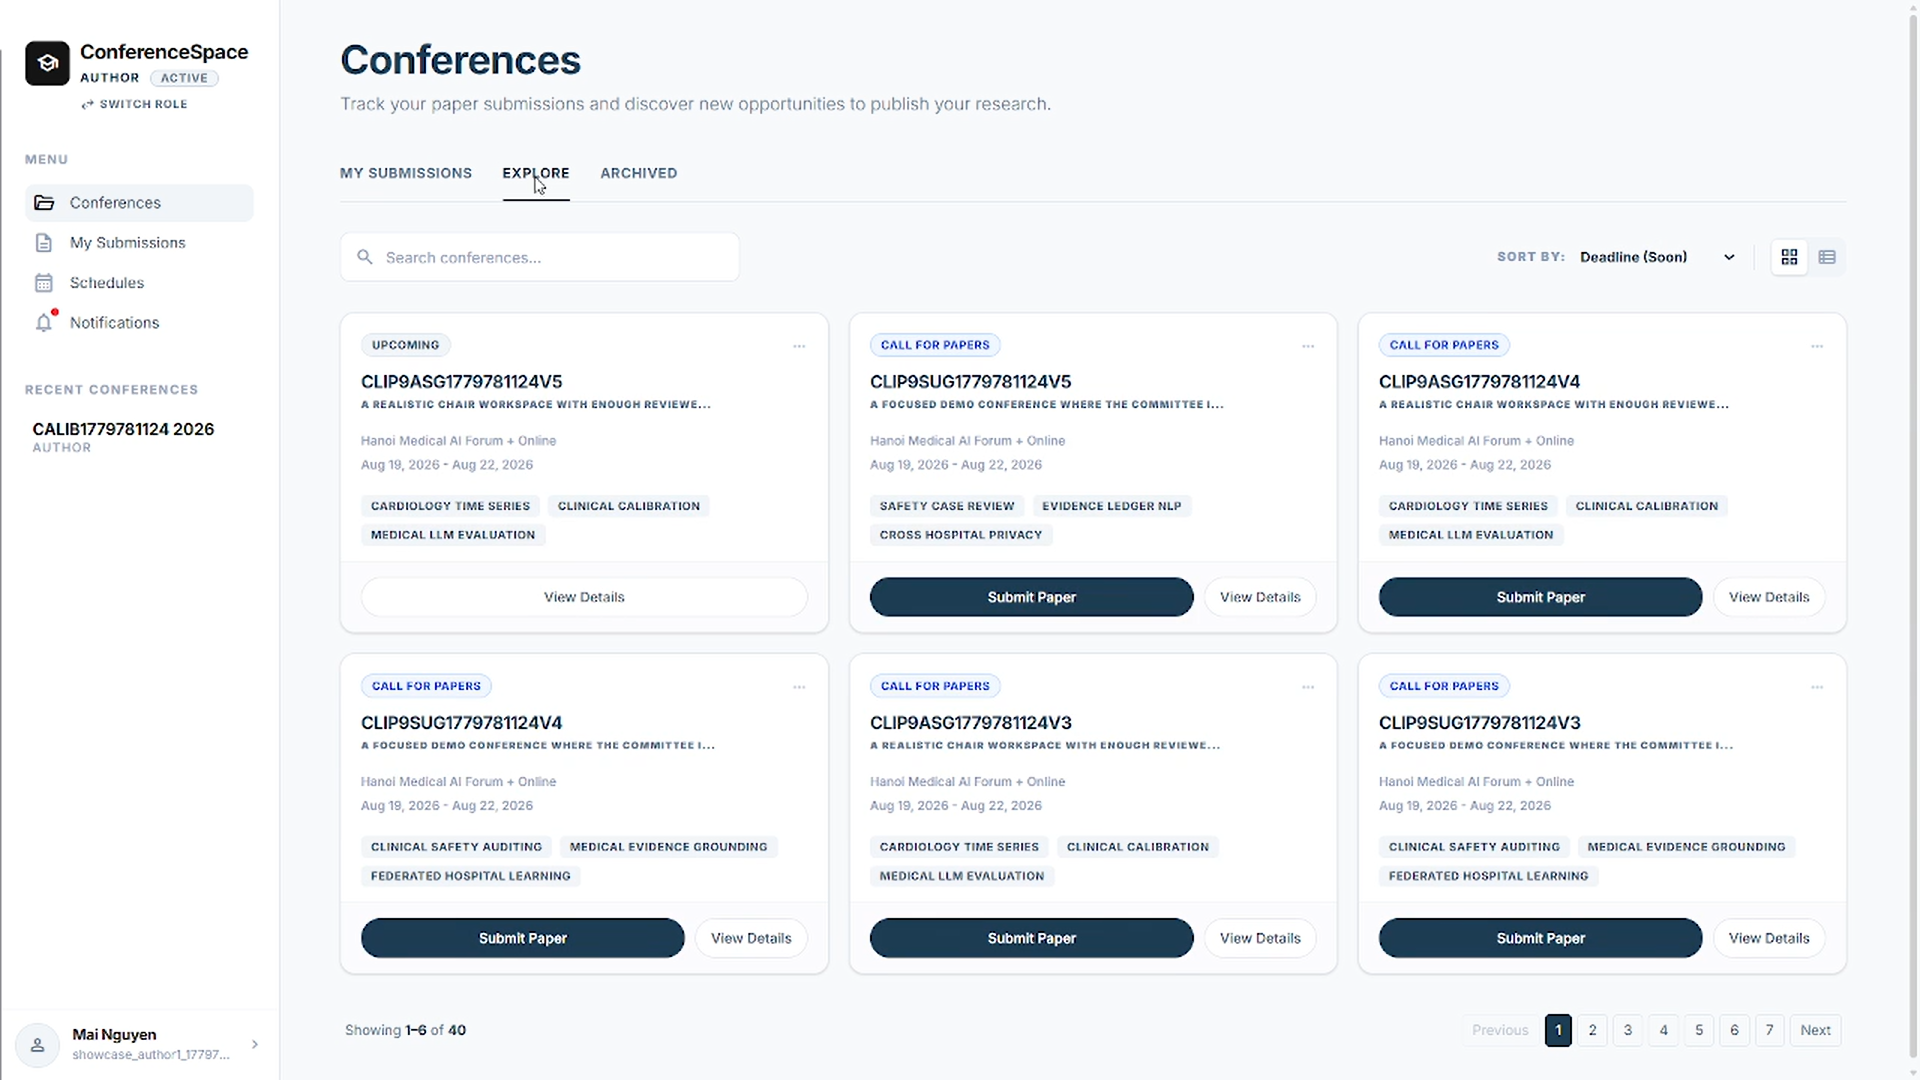
\includegraphics[width=0.95\textwidth]{images/chapter_3_uc01_explore_conferences.png}
  \caption{Giao diện khám phá danh sách hội nghị mặc định}
  \label{fig:uc01-explore-cut}
\end{figure}

Hình~\ref{fig:uc01-explore-cut} minh họa giao diện danh sách hội nghị mặc định mà Tác giả nhìn thấy khi bắt đầu tìm kiếm.

\begin{figure}[H]
  \centering
  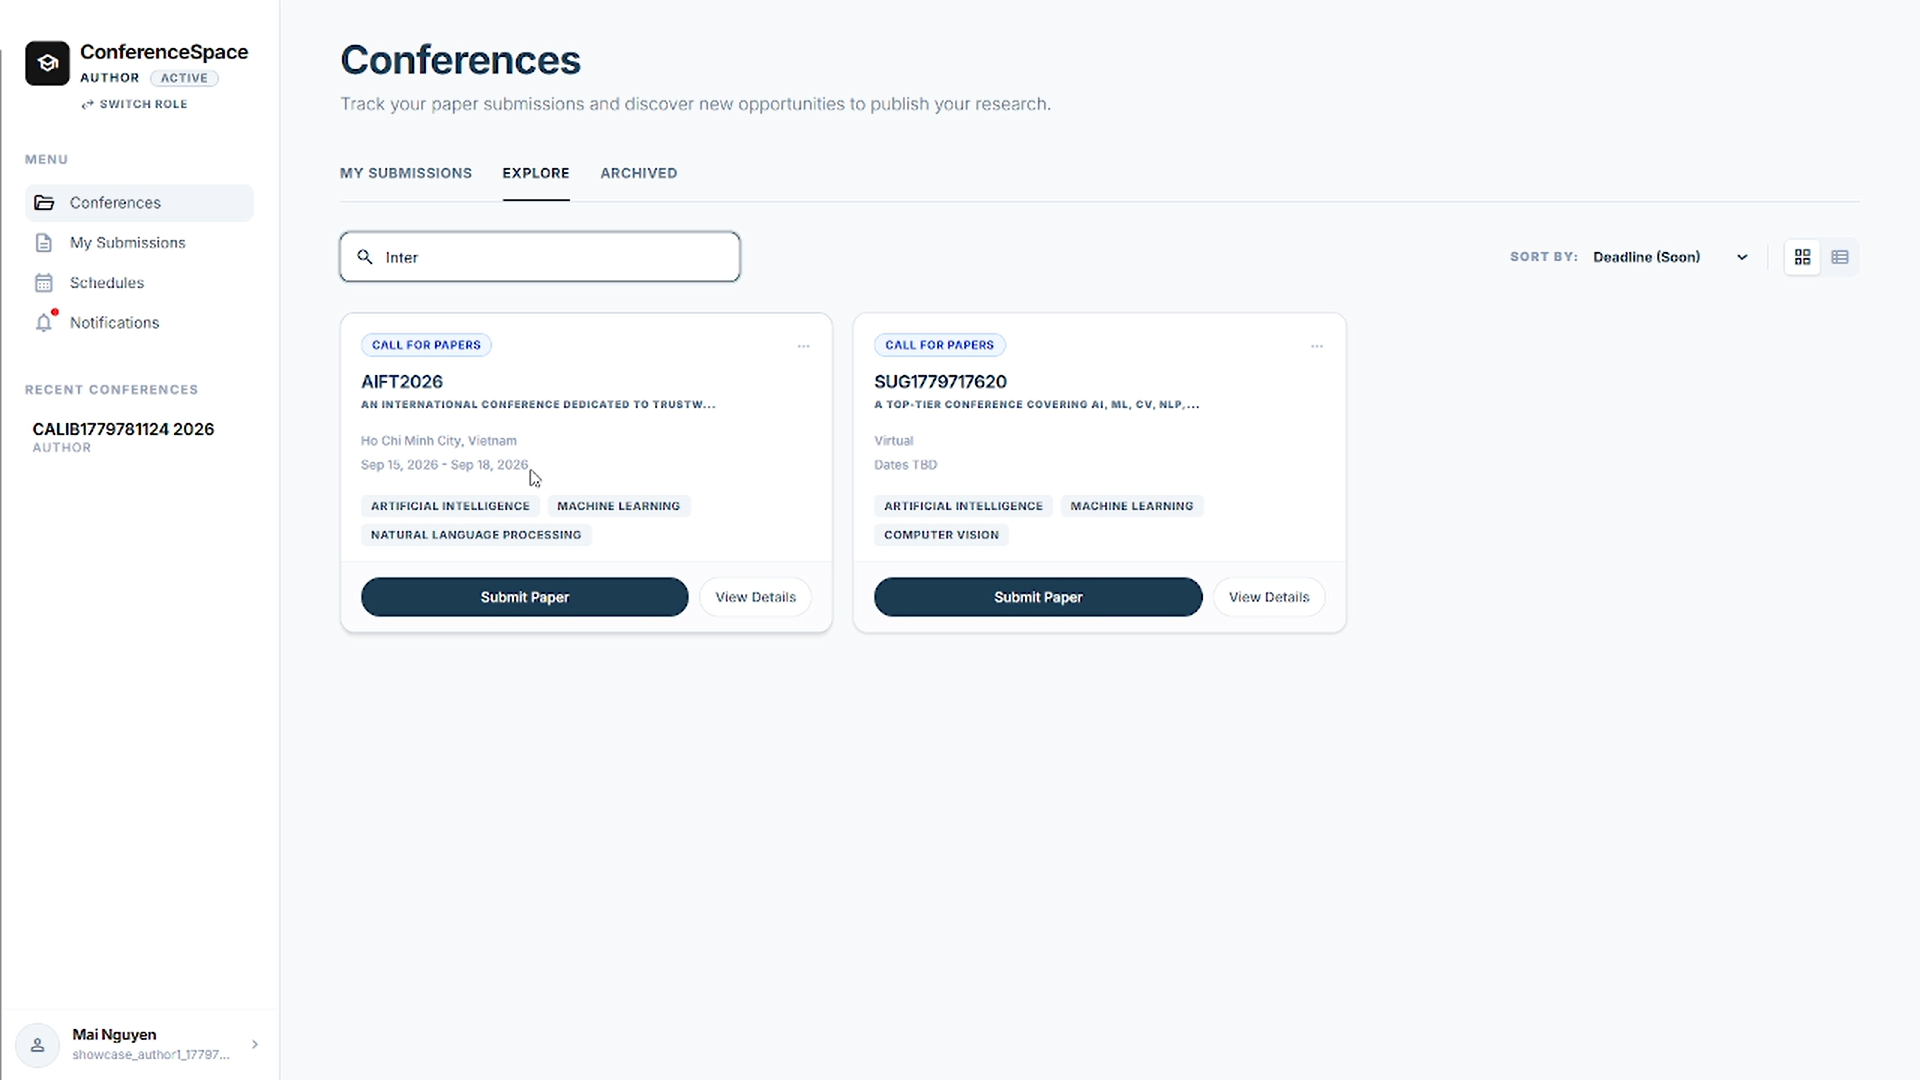
\includegraphics[width=0.95\textwidth]{images/chapter_3_uc01_search_conferences.png}
  \caption{Kết quả tìm kiếm và áp dụng bộ lọc động}
  \label{fig:uc01-search-cut}
\end{figure}

Hình~\ref{fig:uc01-search-cut} minh họa kết quả tìm kiếm sau khi Tác giả áp dụng bộ lọc động.

\begin{figure}[H]
  \centering
  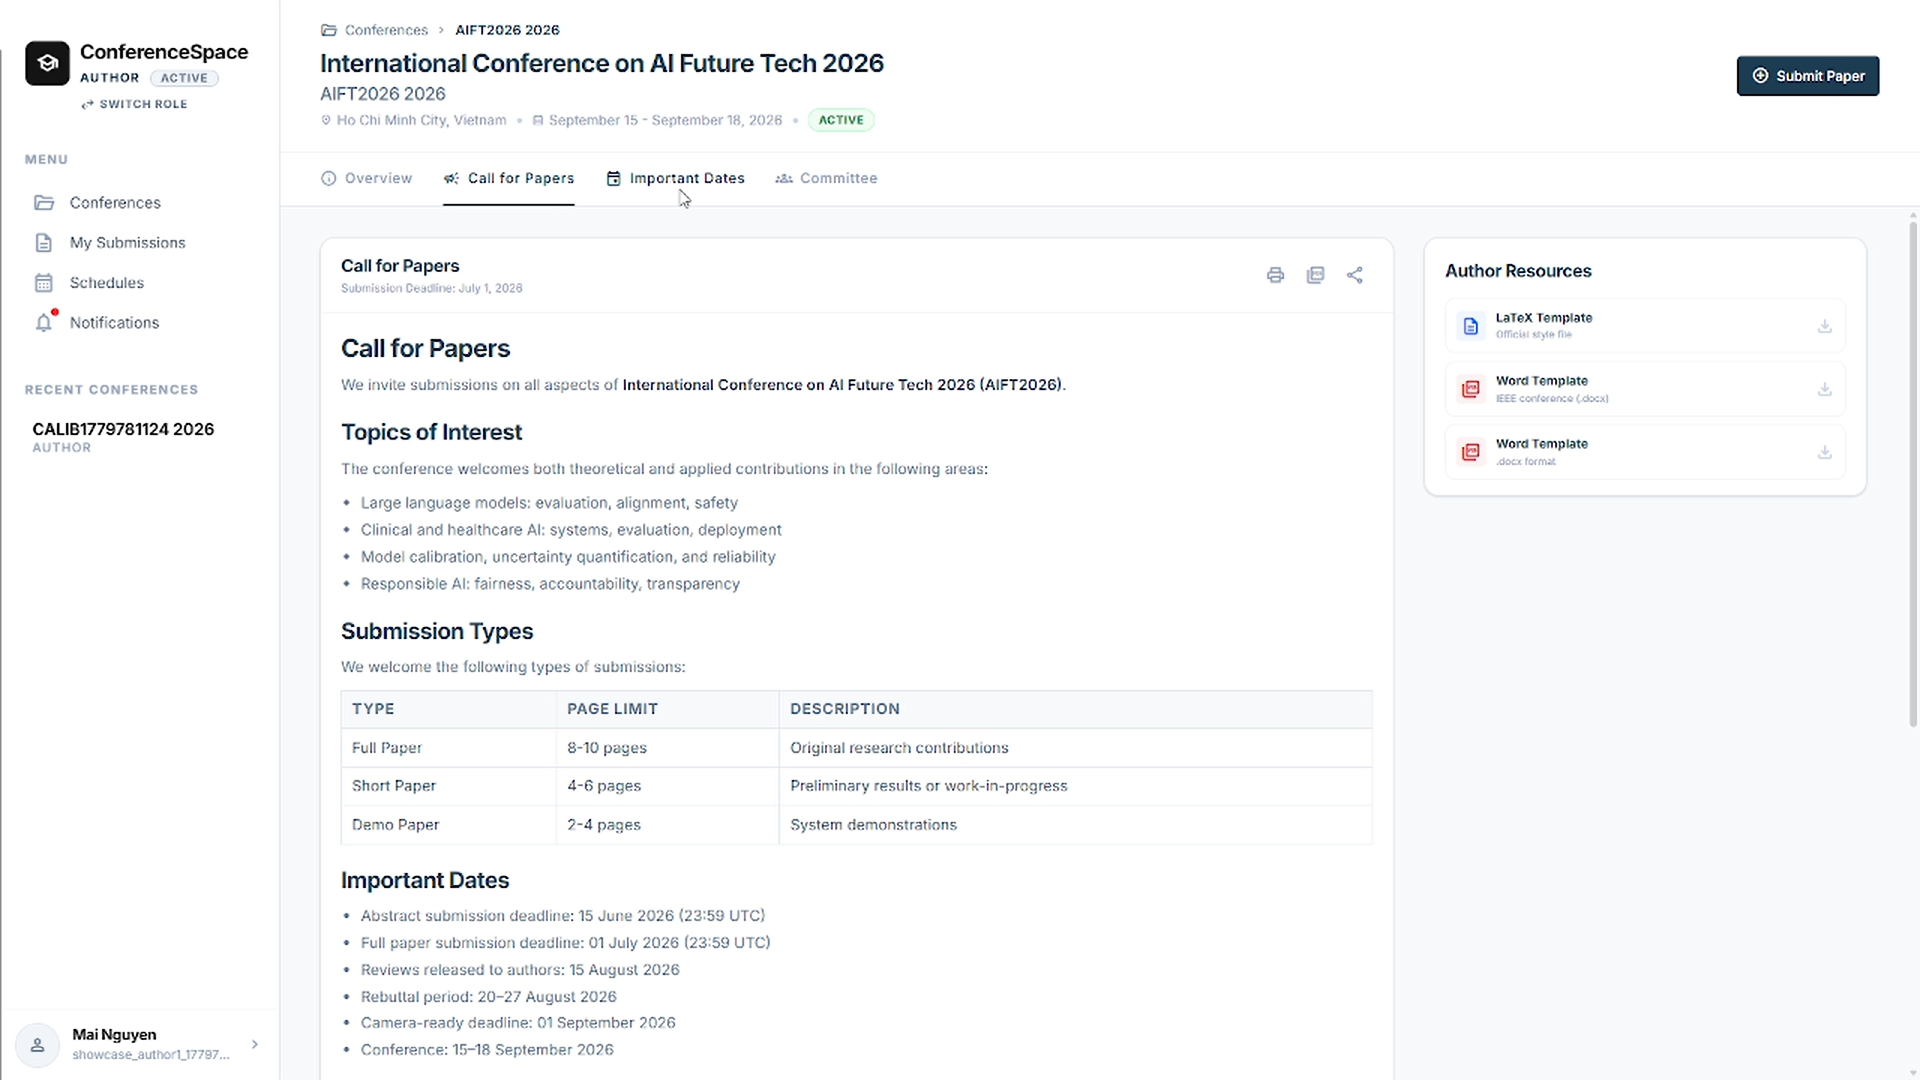
\includegraphics[width=0.95\textwidth]{images/chapter_3_uc01_conference_detail_cfp.png}
  \caption{Giao diện trang chi tiết hội nghị: Tab kêu gọi nộp bài (Call for Papers)}
  \label{fig:uc01-detail-cfp-cut}
\end{figure}

Hình~\ref{fig:uc01-detail-cfp-cut} thể hiện tab kêu gọi nộp bài (Call for Papers) trên trang chi tiết hội nghị.

\begin{figure}[H]
  \centering
  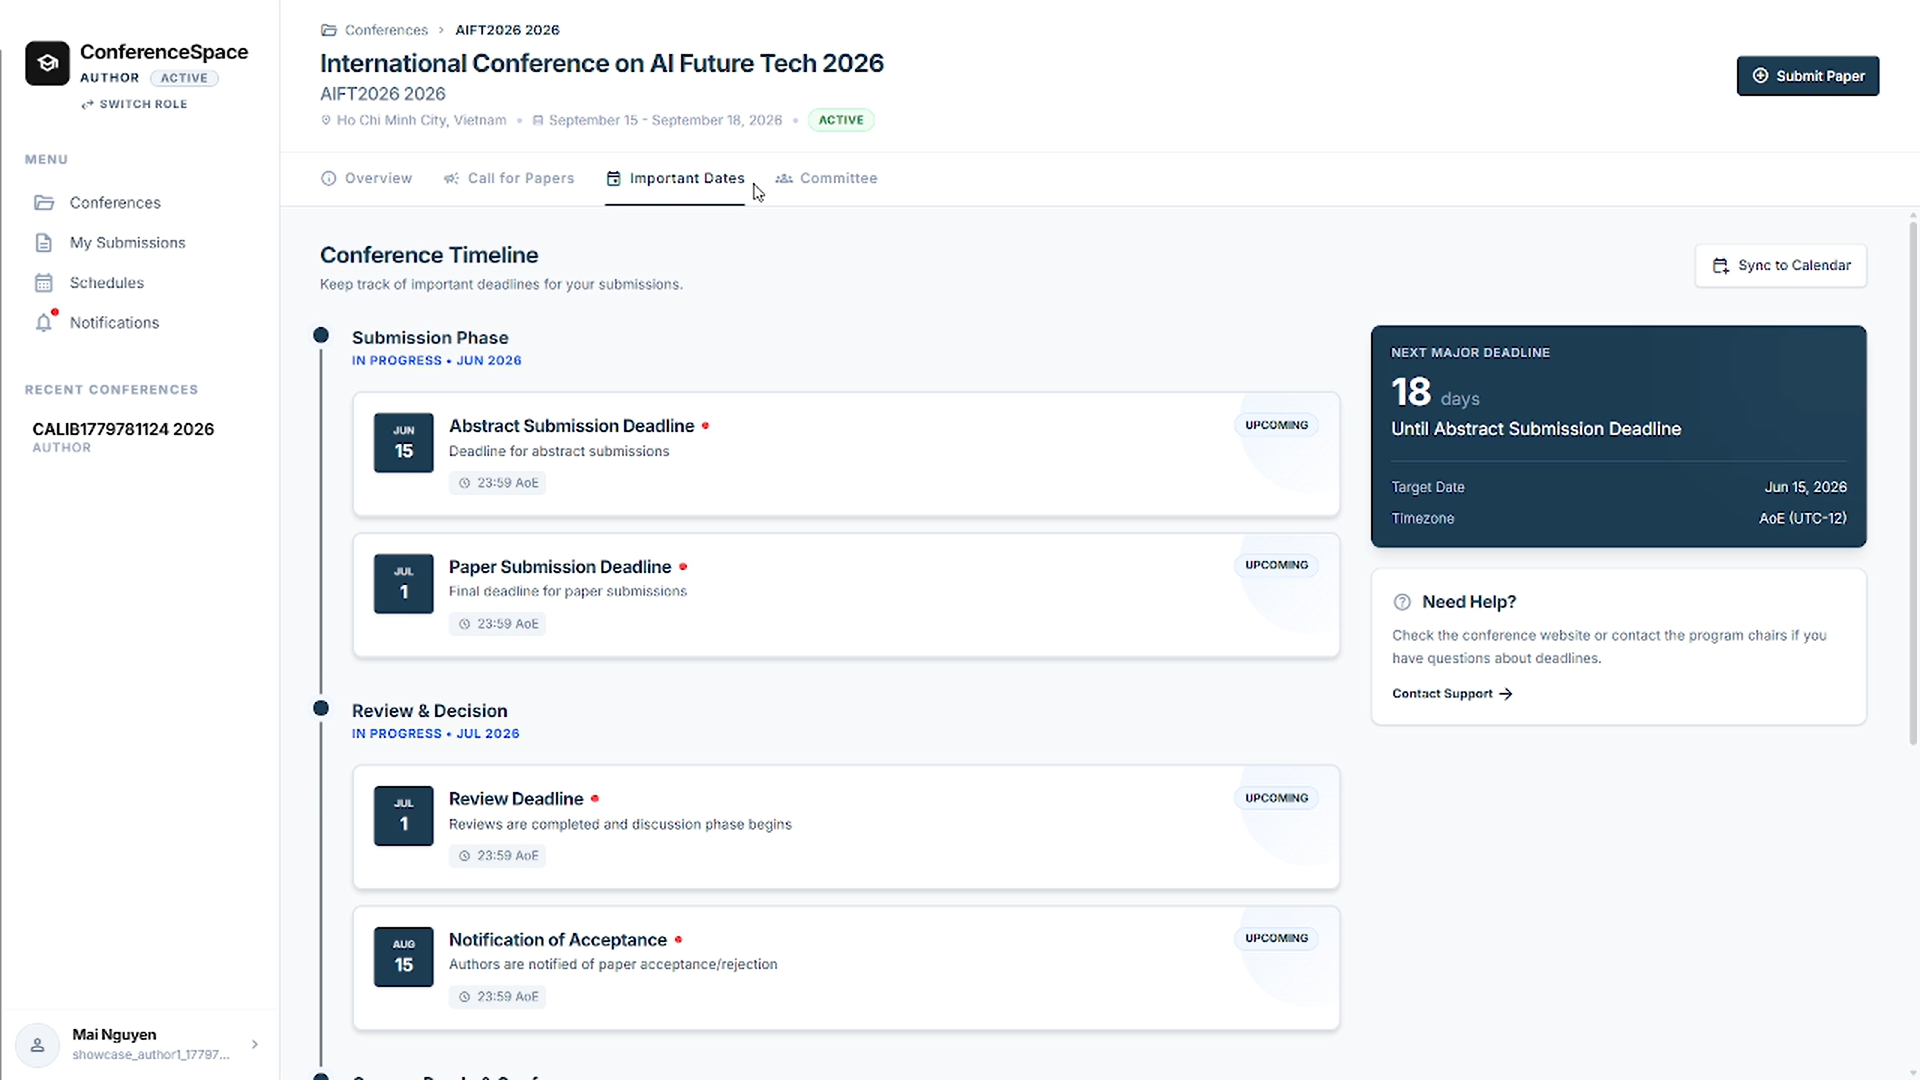
\includegraphics[width=0.95\textwidth]{images/chapter_3_uc01_conference_detail_dates.png}
  \caption{Giao diện trang chi tiết hội nghị: Tab mốc thời gian quan trọng (Important Dates)}
  \label{fig:uc01-detail-dates-cut}
\end{figure}


Hình~\ref{fig:uc01-detail-dates-cut} thể hiện tab mốc thời gian quan trọng trên trang chi tiết hội nghị.

\begin{figure}[H]
  \centering
  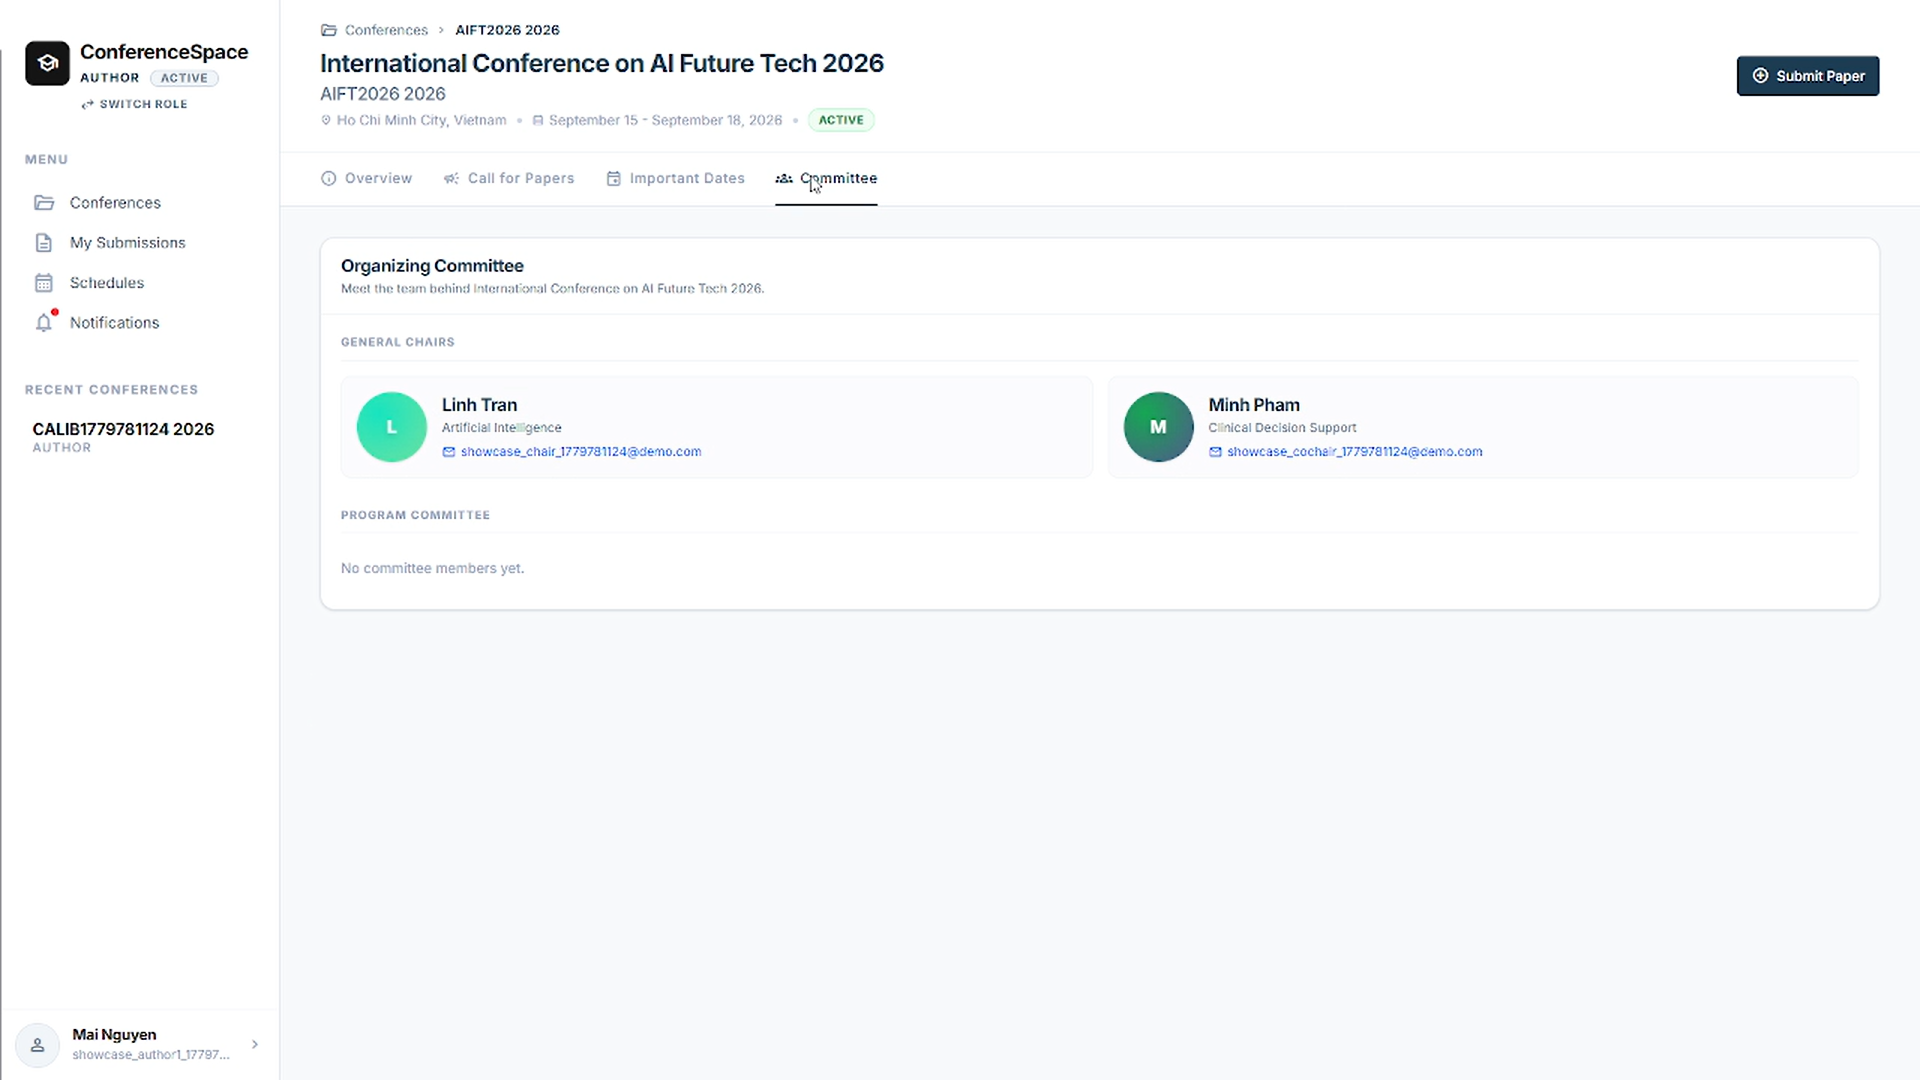
\includegraphics[width=0.95\textwidth]{images/chapter_3_uc01_conference_detail_committee.png}
  \caption{Giao diện trang chi tiết hội nghị: tab hội đồng chương trình (Committee)}
  \label{fig:uc01-detail-committee-cut}
\end{figure}

Hình~\ref{fig:uc01-detail-committee-cut} thể hiện tab hội đồng chương trình trên trang chi tiết hội nghị.

\begin{figure}[H]
  \centering
  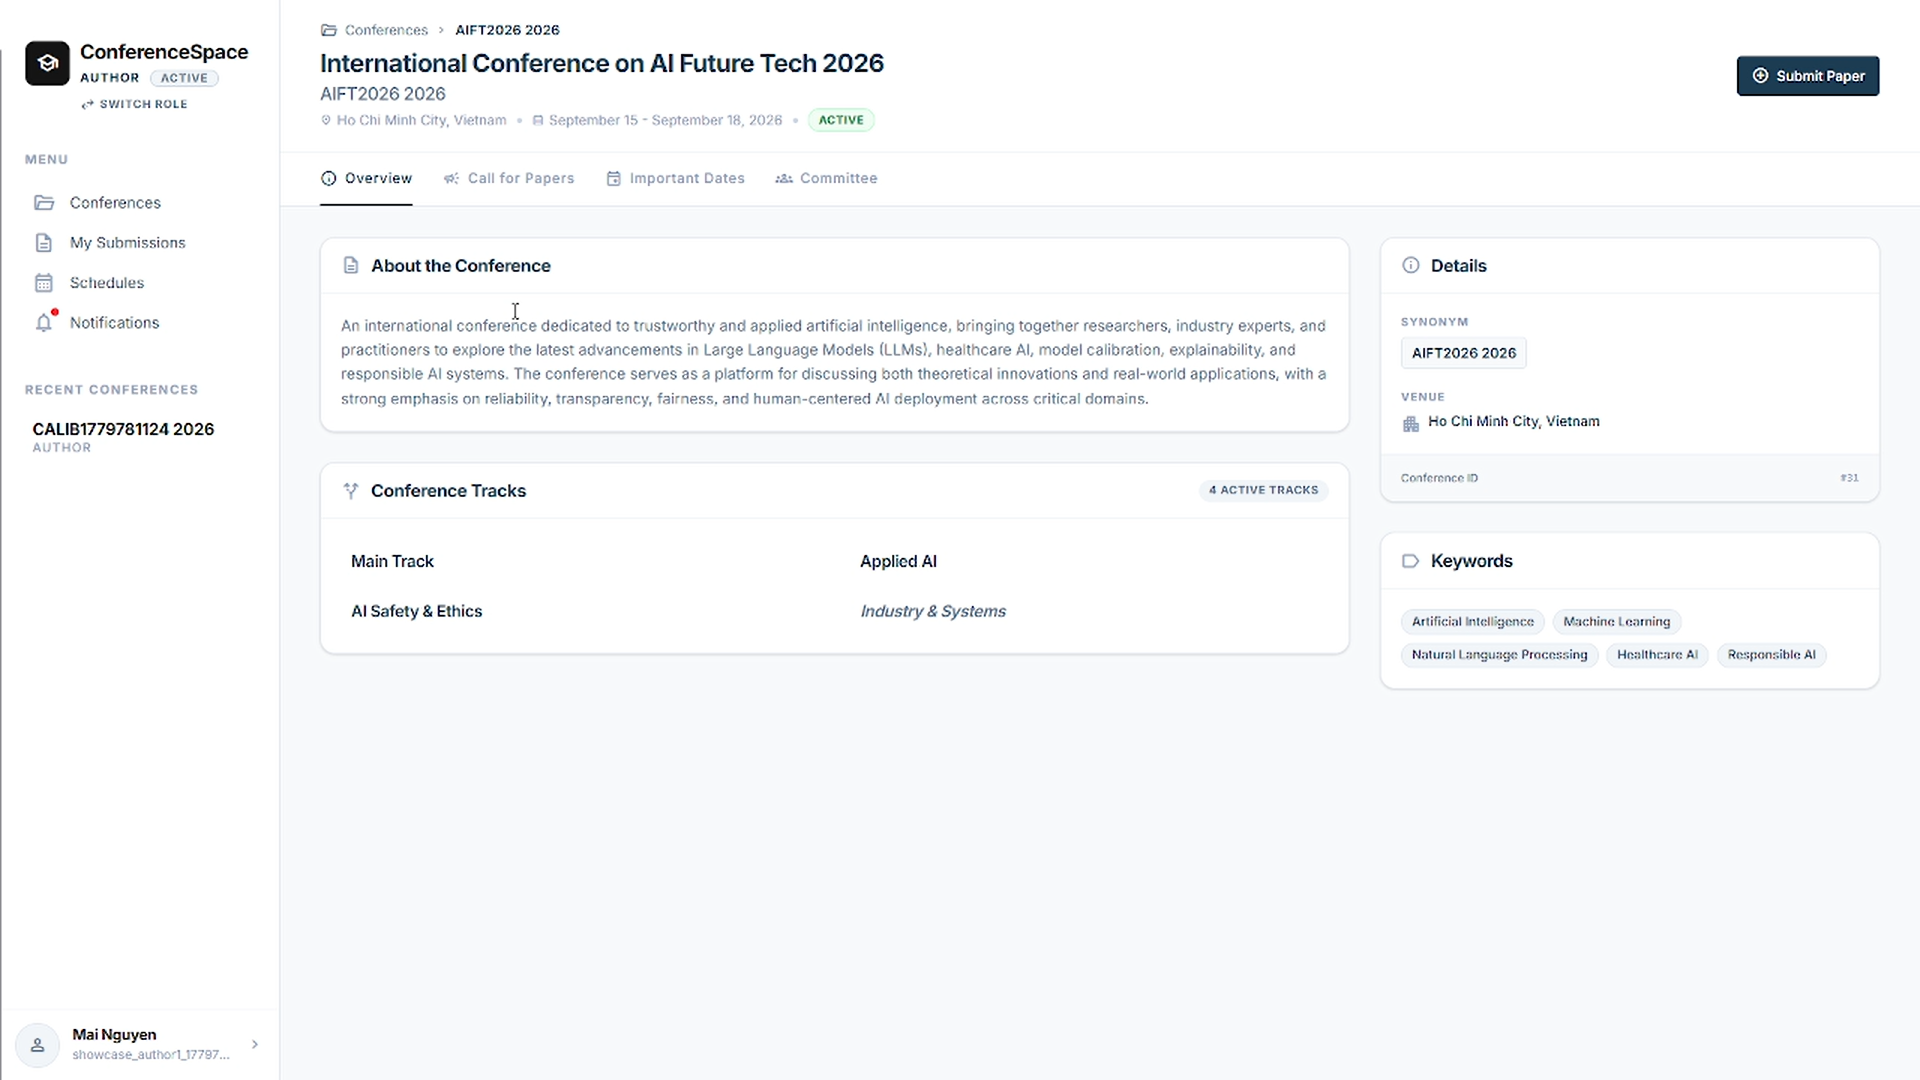
\includegraphics[width=0.95\textwidth]{images/chapter_3_uc01_conference_detail_overview.png}
  \caption{Giao diện trang chi tiết hội nghị: Tab tổng quan (Overview)}
  \label{fig:uc01-detail-overview-cut}
\end{figure}

Hình~\ref{fig:uc01-detail-overview-cut} thể hiện tab tổng quan của trang chi tiết hội nghị mà Tác giả xem trước khi quyết định nộp bài hoặc lưu theo dõi.

\subsubsection{UC-02. Hoàn tất và kiểm tra bài nộp}

Tác giả tạo bản nháp, tải bản thảo và có thể yêu cầu Submission Autofill trích xuất siêu dữ liệu cùng gợi ý chuyên đề trong danh sách hợp lệ. Tác giả kiểm tra, chỉnh sửa thông tin, khai báo đồng tác giả và xung đột lợi ích trước khi Submission Gating kiểm tra tệp, chính sách và các điều kiện gửi bài. Trạng thái \textit{warn} cho phép tiếp tục khi chính sách hội nghị cho phép; trạng thái \textit{block} ngăn gửi cho đến khi lỗi có căn cứ được khắc phục. Nếu Submission Autofill không khả dụng, Tác giả vẫn có thể nhập và lưu bản nháp thủ công. Nếu Submission Gating không trả được bất kỳ kết quả hợp lệ nào, backend chưa cho phép gửi bài cho đến khi thực hiện được một lần kiểm tra hợp lệ.

\begin{figure}[H]
  \centering
  \begin{minipage}{0.48\textwidth}
    \centering
    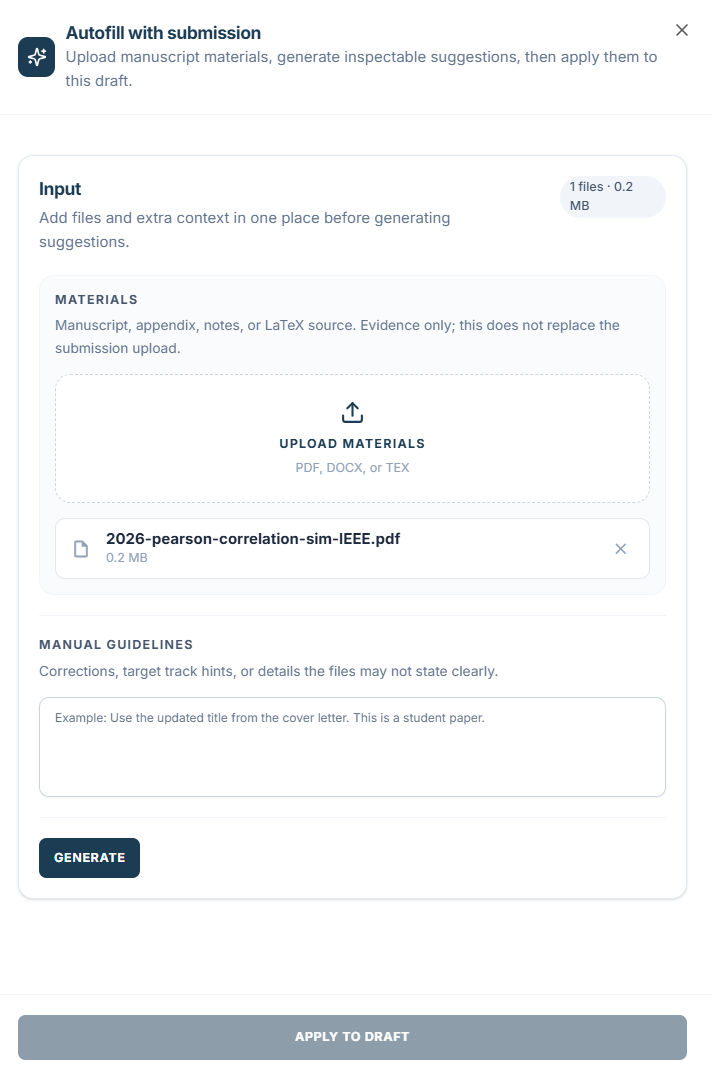
\includegraphics[width=0.56\textwidth]{images/chapter_3_uc02_autofill_1.png}
  \end{minipage}
  \begin{minipage}{0.48\textwidth}
    \centering
    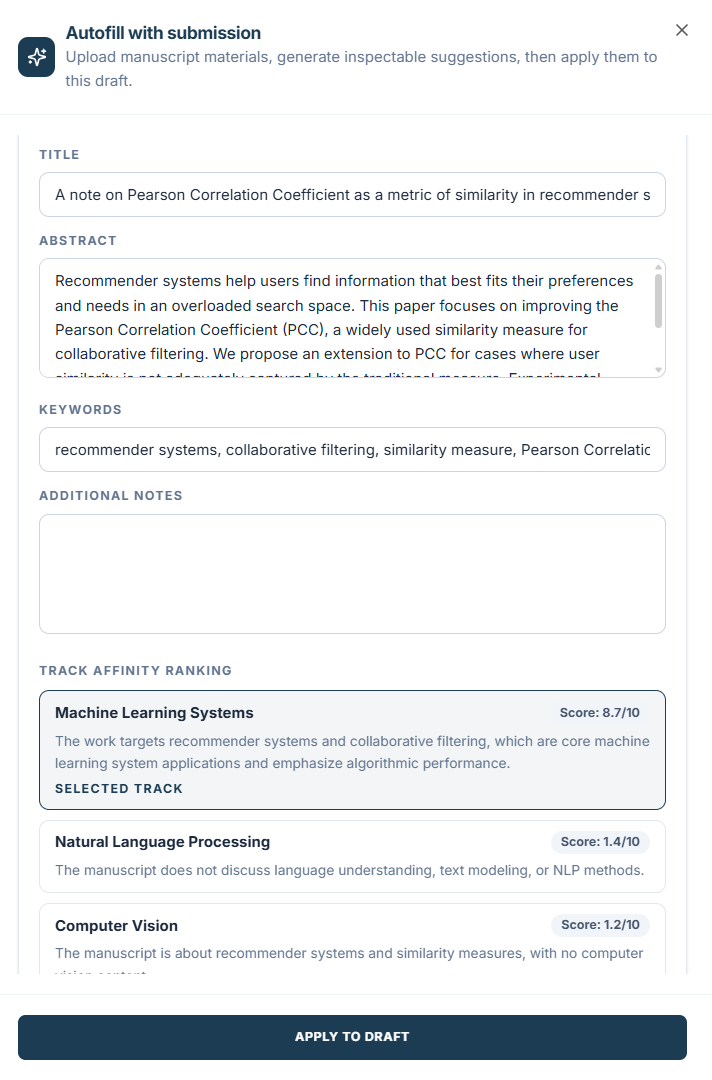
\includegraphics[width=0.56\textwidth]{images/chapter_3_uc02_autofill_2.png}
  \end{minipage}
  \caption{Giao diện tải lên bản thảo (trái) và kết quả trích xuất thông tin tự động (phải)}
  \label{fig:uc02-autofill-cut}
\end{figure}

Hình~\ref{fig:uc02-autofill-cut} trình bày giao diện tải lên bản thảo (trái) cùng kết quả trích xuất thông tin mà Submission Autofill trả về (phải) để Tác giả kiểm tra và chỉnh sửa.

\begin{figure}[H]
  \centering
  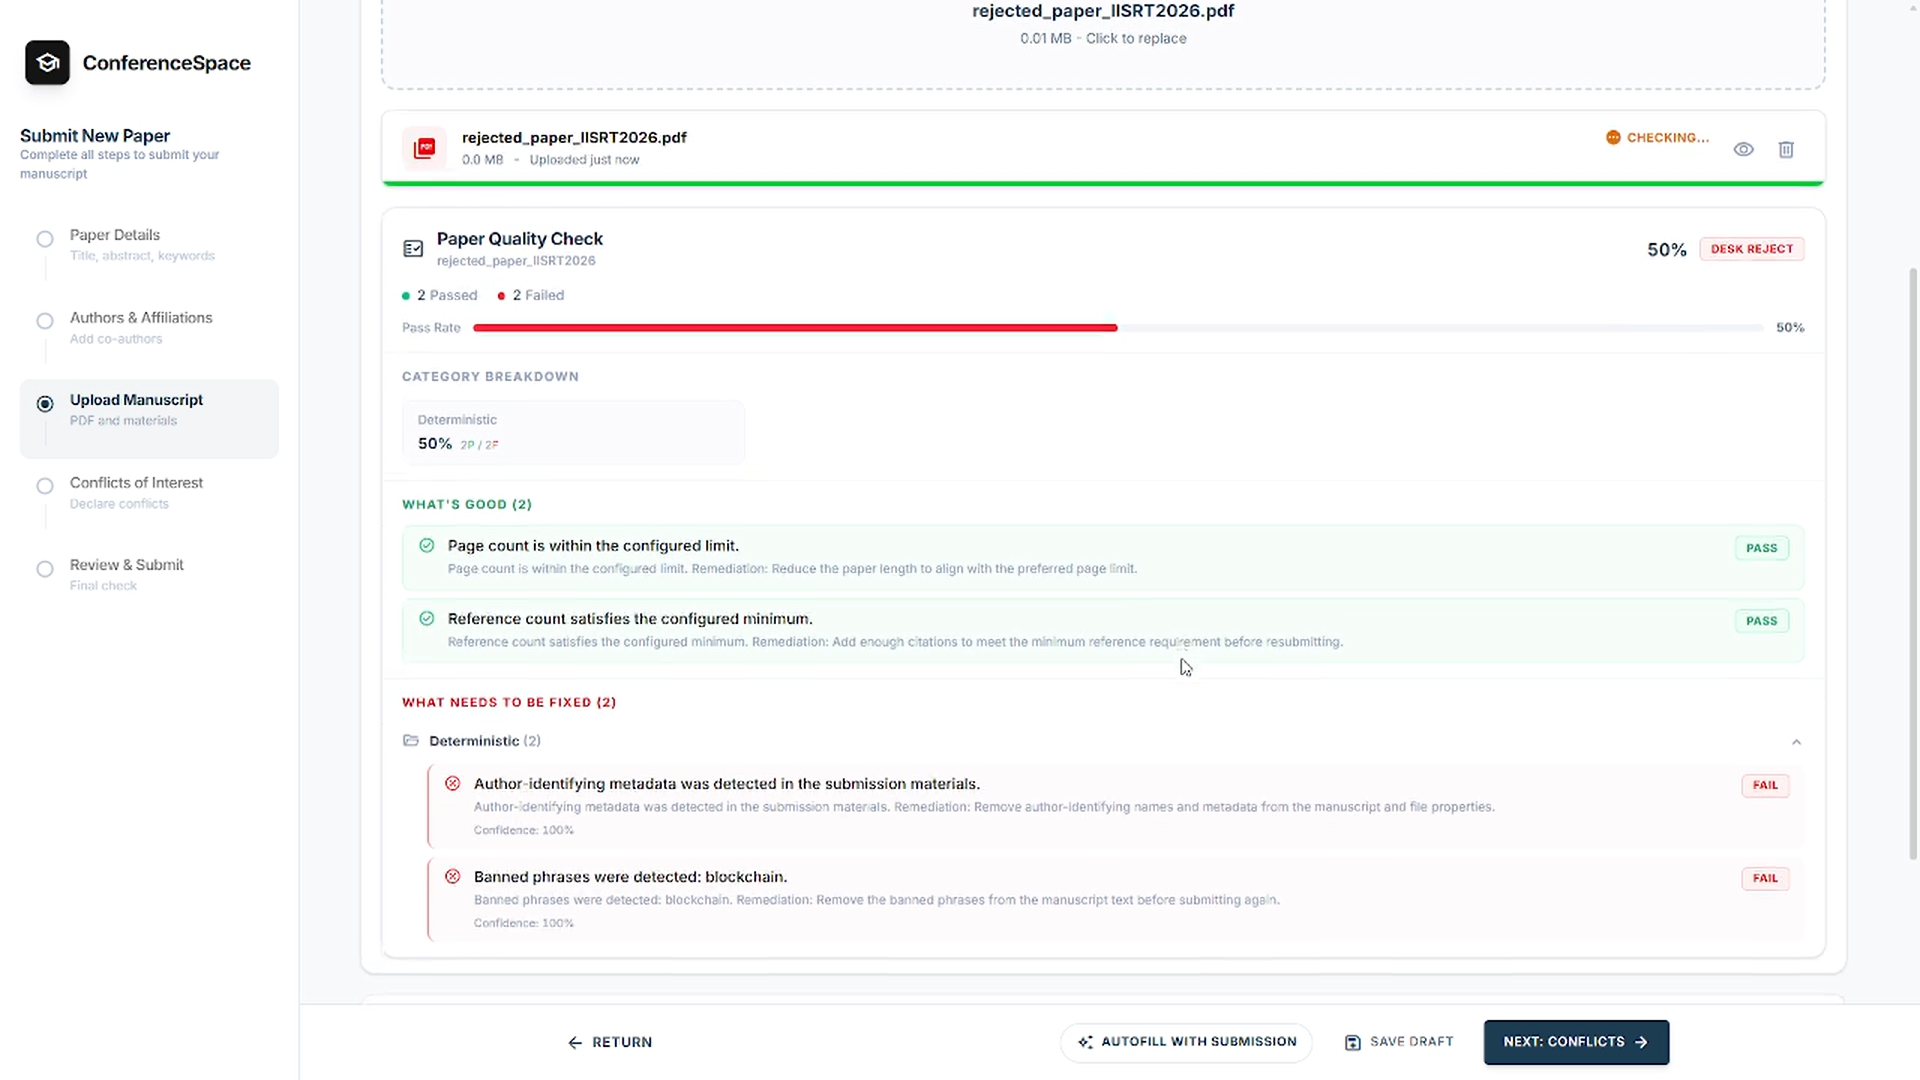
\includegraphics[width=0.95\textwidth]{images/chapter_3_uc02_precheck_gating.png}
  \caption{Kết quả Submission Gating theo ba trạng thái \textit{pass}, \textit{warn} và \textit{block}}
  \label{fig:uc02-gating-cut}
\end{figure}

Trước khi gửi bài, Tác giả xem kết quả kiểm tra tự động của Submission Gating tại Hình~\ref{fig:uc02-gating-cut}, gồm ba trạng thái \textit{pass}, \textit{warn} và \textit{block}.

\begin{figure}[H]
  \centering
  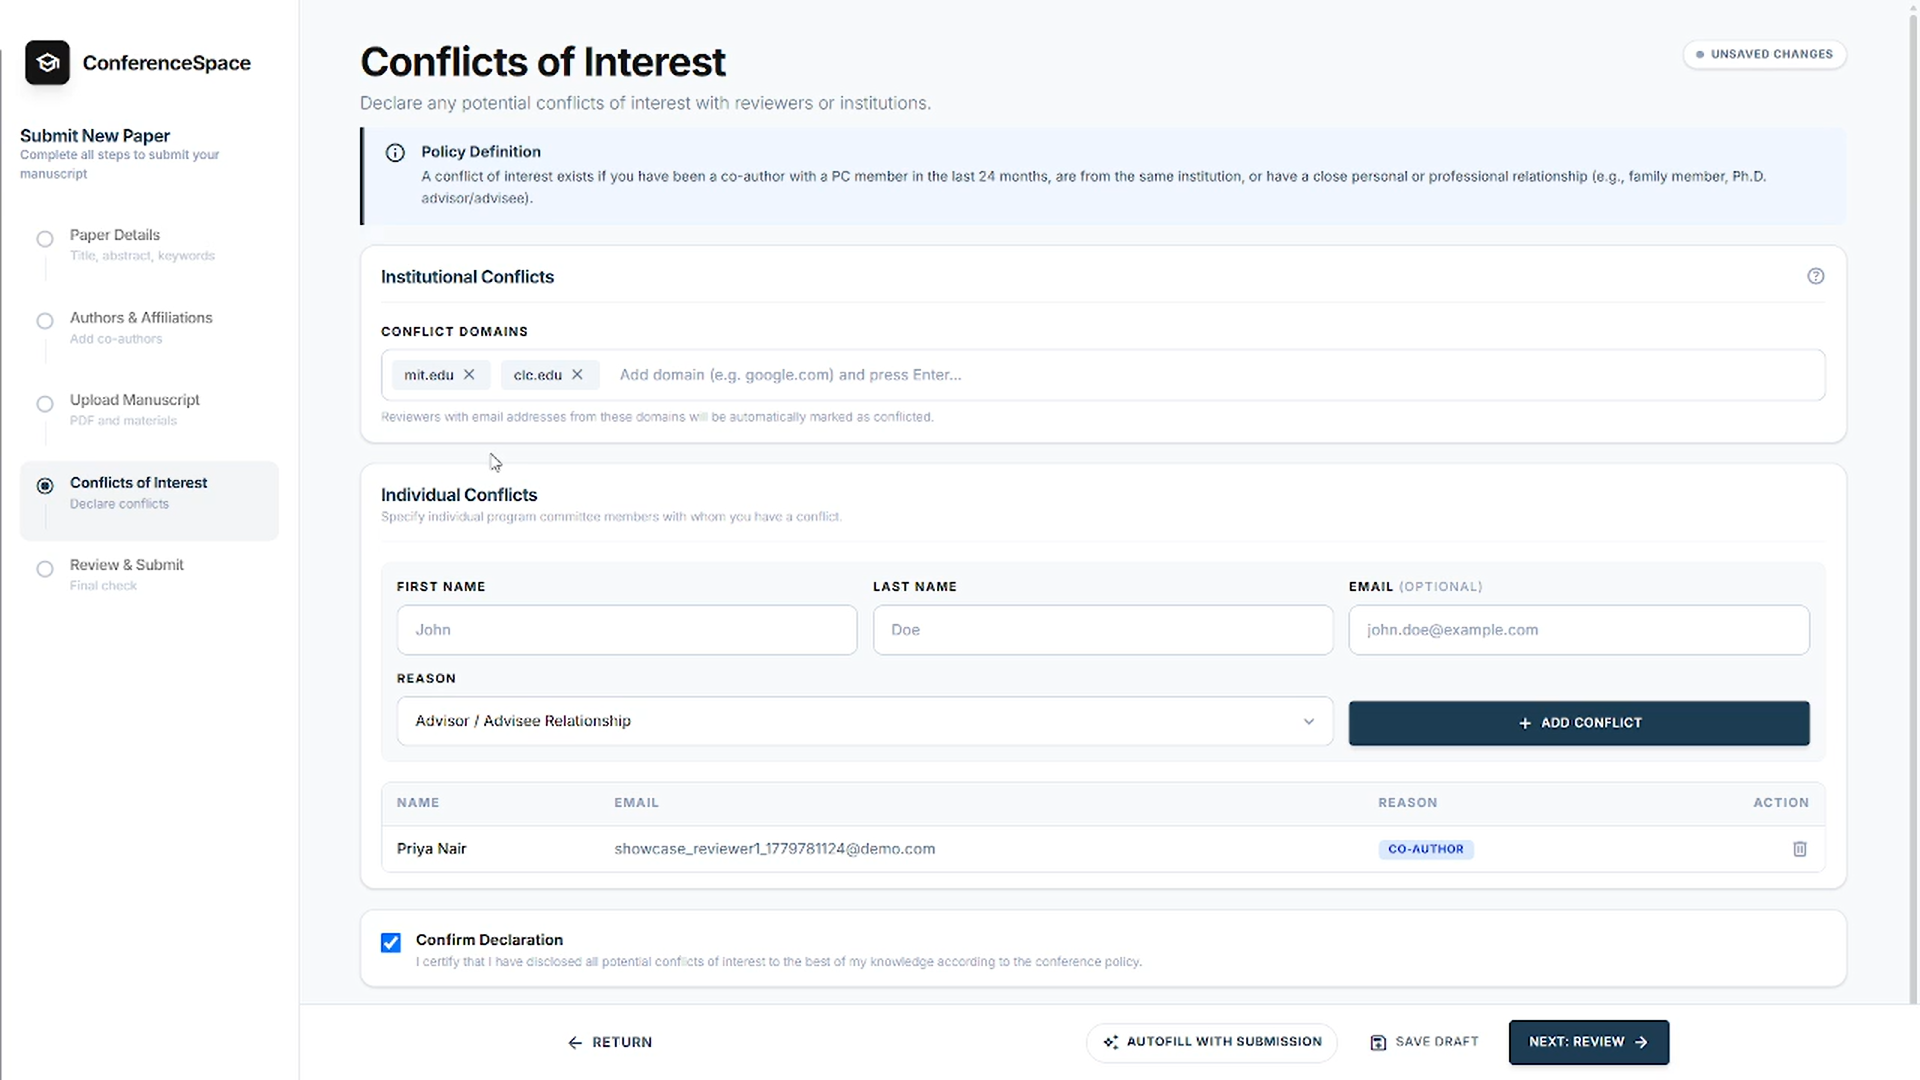
\includegraphics[width=0.95\textwidth]{images/chapter_3_uc02_authors_conflict.png}
  \caption{Giao diện khai báo thông tin các đồng tác giả và xung đột lợi ích}
  \label{fig:uc02-authors-conflict-cut}
\end{figure}

Hình~\ref{fig:uc02-authors-conflict-cut} minh họa giao diện khai báo đồng tác giả và xung đột lợi ích mà Tác giả hoàn tất trước khi Submission Gating kiểm tra.

Hai chức năng AI chỉ hỗ trợ hoàn tất bài nộp: Submission Autofill tạo bản nháp có thể sửa, còn Submission Gating kiểm tra điều kiện trước khi gửi. Tác giả vẫn là người xác nhận dữ liệu và thực hiện thao tác gửi chính thức.

\subsubsection{UC-03. Quản lý vòng đời bài nộp}

Sau khi tạo bài, Tác giả theo dõi và thực hiện các hành động phù hợp với từng trạng thái: chỉnh sửa bản nháp; theo dõi hoặc rút bài đã gửi khi cấu hình và hạn chót nộp bài cho phép; xem phản biện khi được công bố; gửi phản hồi trong giai đoạn do Chủ tọa hoặc Đồng chủ tọa mở; và tải bản thảo hoàn chỉnh khi bài được chấp nhận. Backend từ chối yêu cầu không phù hợp với trạng thái hoặc hạn chót tương ứng. Phiên bản hiện tại hỗ trợ tải và truy xuất bản thảo hoàn chỉnh nhưng chưa có luồng để Chủ tọa phê duyệt, yêu cầu nộp lại hoặc kiểm tra hạn chót nộp bản thảo hoàn chỉnh tại thời điểm thực thi.

\begin{figure}[H]
  \centering
  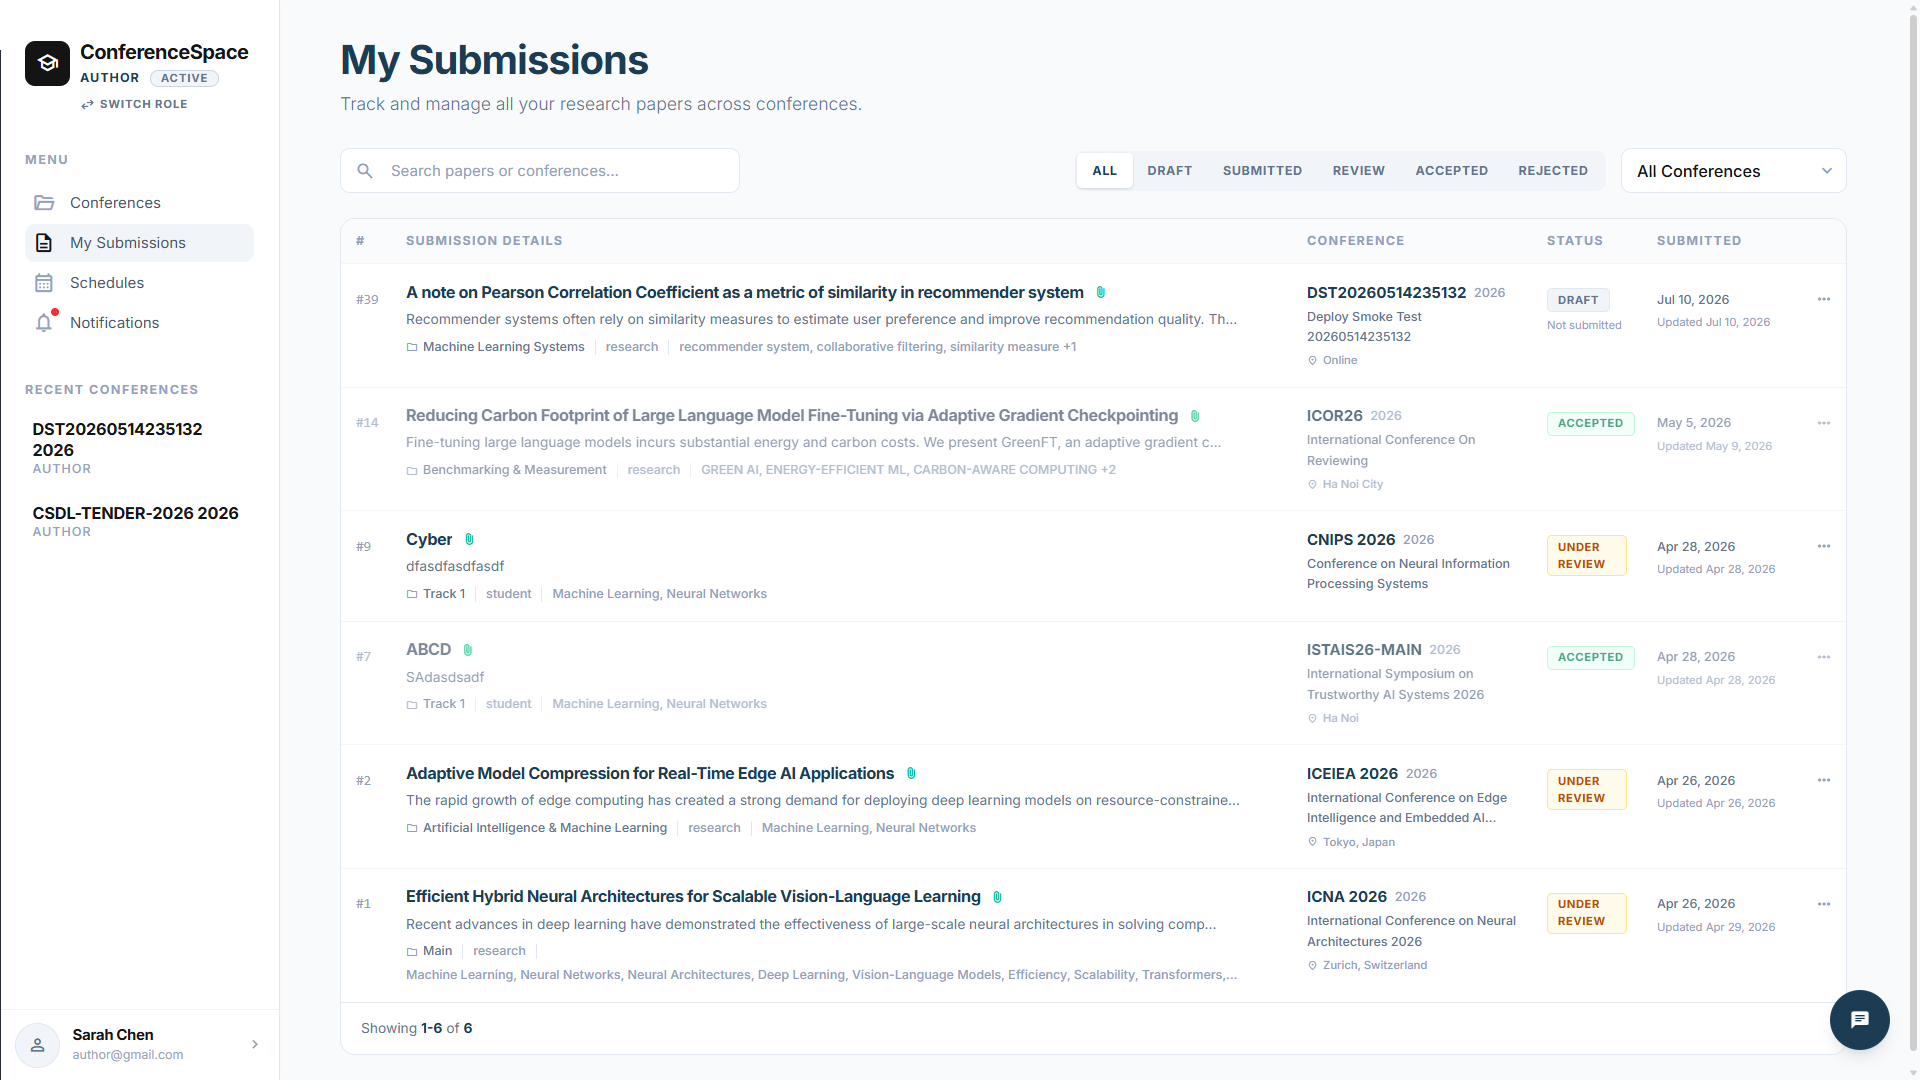
\includegraphics[width=0.95\textwidth]{images/chapter_3_uc03_submissions_list.png}
  \caption{Danh sách bài nộp và trạng thái vòng đời trong không gian làm việc của Tác giả}
  \label{fig:uc03-submissions-cut}
\end{figure}

Giao diện ở Hình~\ref{fig:uc03-submissions-cut} cung cấp một điểm nhìn thống nhất để Tác giả nhận biết trạng thái hiện hành và thao tác nghiệp vụ còn hợp lệ, thay vì chỉ minh họa riêng các chức năng AI ở bước chuẩn bị bài.

\begin{figure}[H]
  \centering
  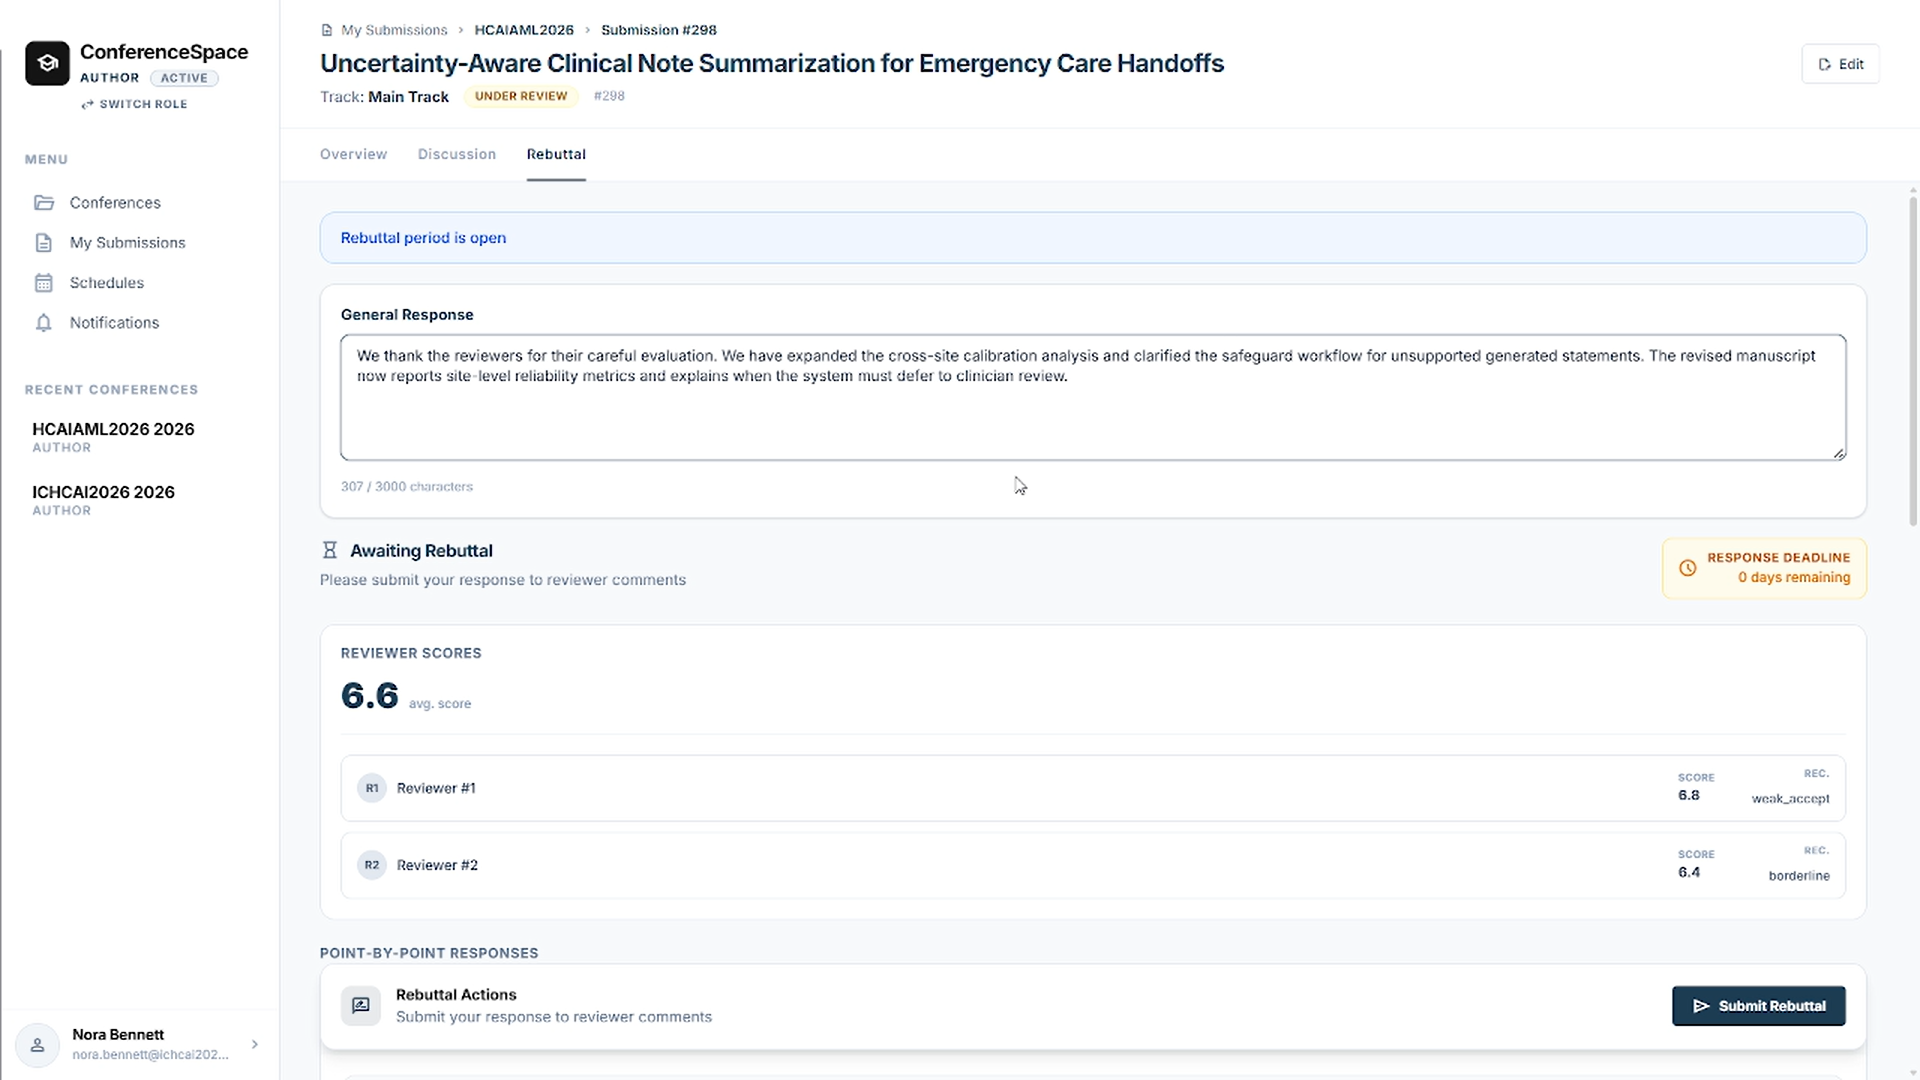
\includegraphics[width=0.95\textwidth]{images/chapter_3_uc03_rebuttal.png}
  \caption{Giao diện soạn thảo và gửi phản hồi của tác giả (rebuttal)}
  \label{fig:uc03-rebuttal-cut}
\end{figure}

Hình~\ref{fig:uc03-rebuttal-cut} minh họa giao diện Tác giả soạn và gửi phản hồi (rebuttal) trong giai đoạn phản hồi.

\begin{figure}[H]
  \centering
  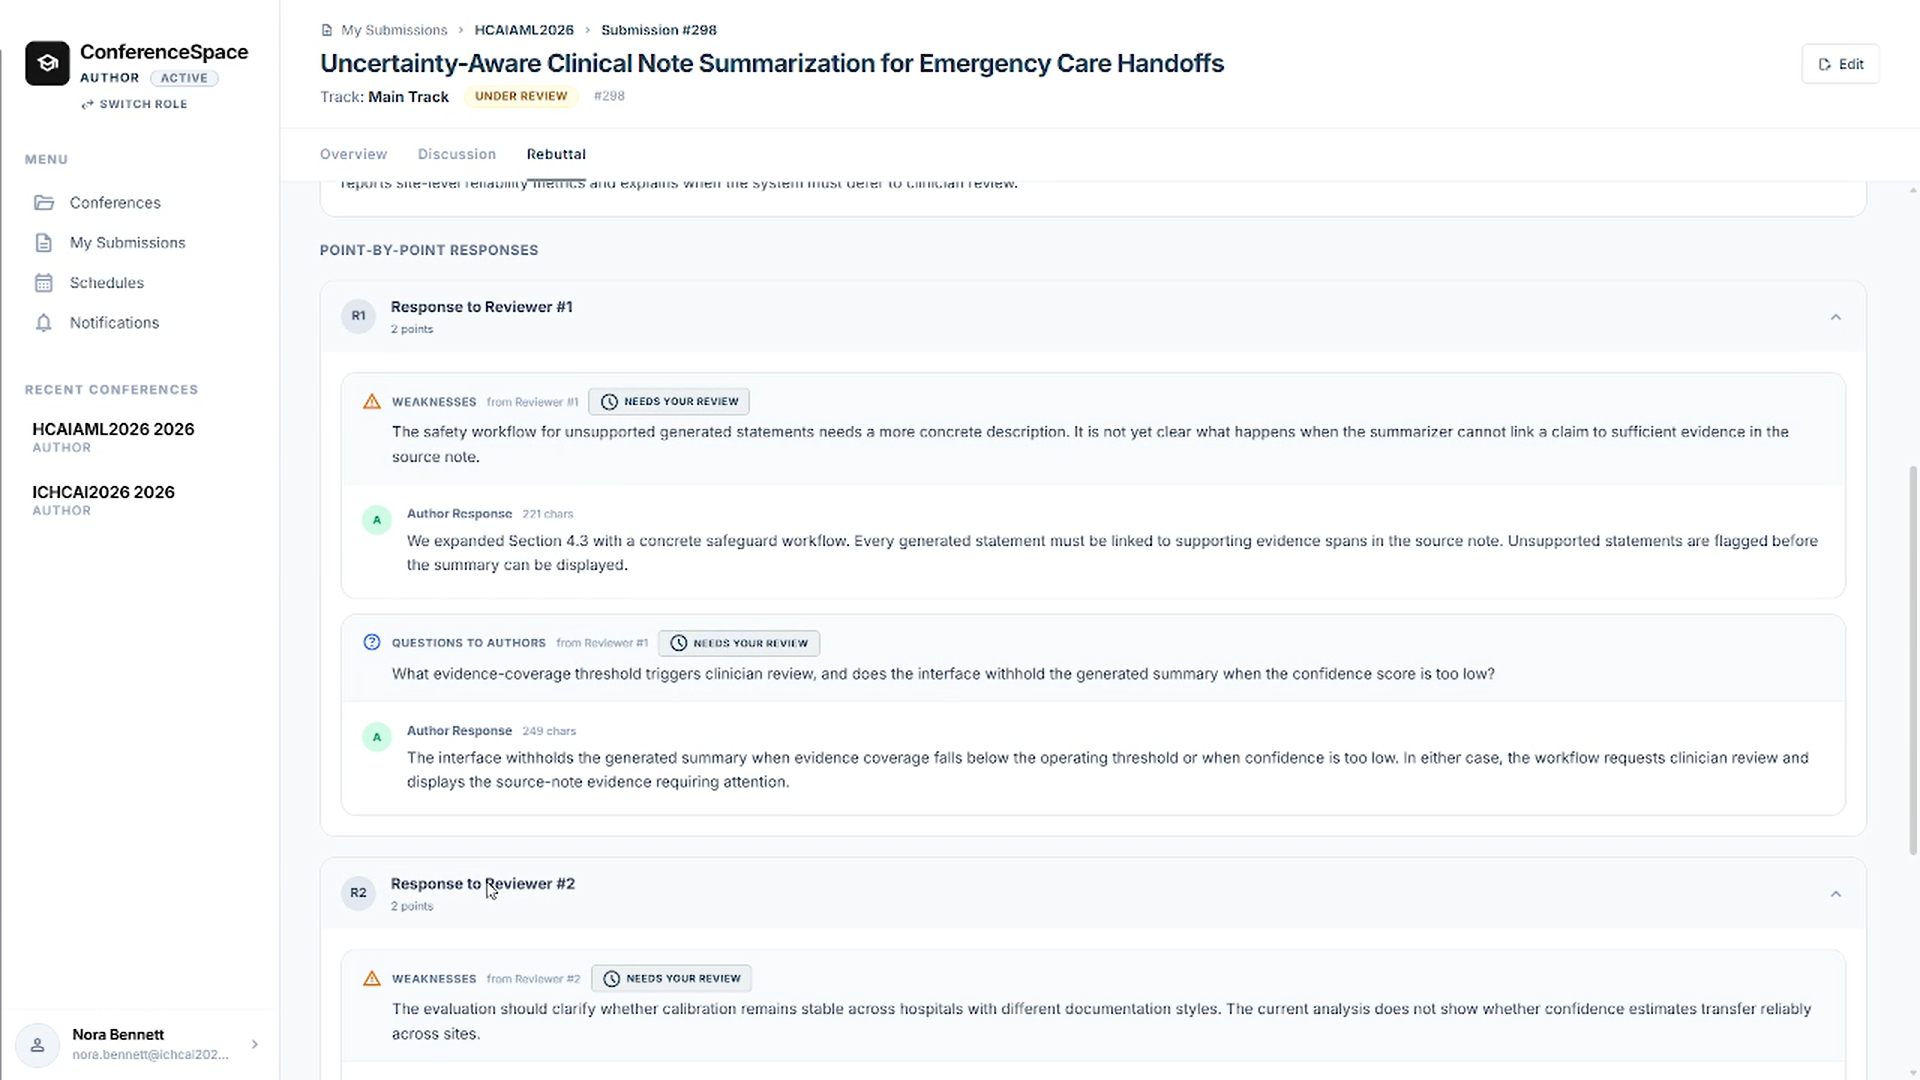
\includegraphics[width=0.95\textwidth]{images/chapter_3_uc03_rebuttal_2.png}
  \caption{Biến thể giao diện soạn và gửi phản hồi của Tác giả (rebuttal)}
  \label{fig:uc03-rebuttal-2-cut}
\end{figure}

Hình~\ref{fig:uc03-rebuttal-2-cut} trình bày một biến thể khác của giao diện soạn thảo và gửi phản hồi.

\begin{figure}[H]
  \centering
  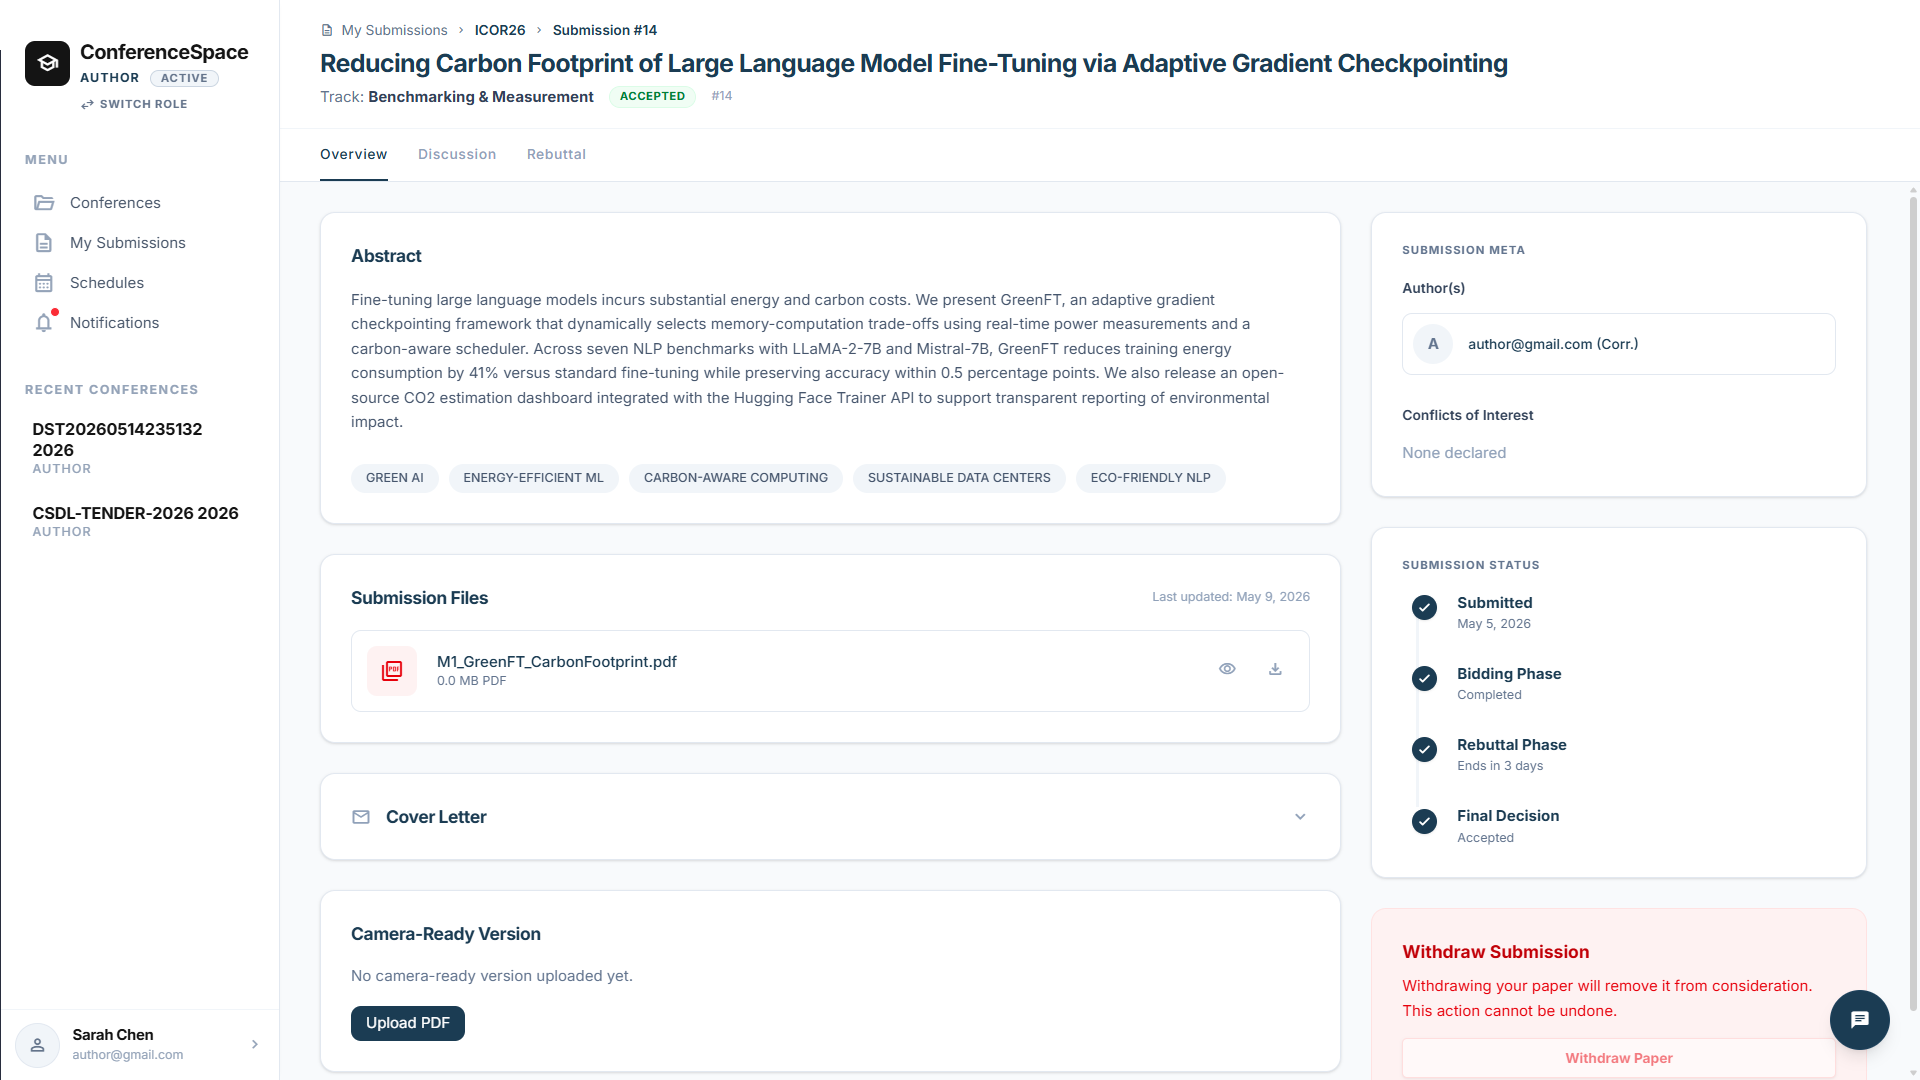
\includegraphics[width=0.95\textwidth]{images/chapter_3_uc03_submission_detail.png}
  \caption{Giao diện trang chi tiết bài nộp, xem nhận định chuyên môn và tải bản thảo hoàn chỉnh (camera-ready)}
  \label{fig:uc03-submission-detail-cut}
\end{figure}

Hình~\ref{fig:uc03-submission-detail-cut} thể hiện trang chi tiết bài nộp, nơi Tác giả xem nhận định chuyên môn và tải lên bản chỉnh sửa cuối cùng khi bài được chấp nhận.

\subsubsection{UC-04. Tiếp nhận lời mời hội nghị và xem bài được phân công}

Chủ tọa gửi lời mời tham gia hội nghị; hệ thống lưu trạng thái và thông báo cho người nhận. Phản biện viên chỉ có thể chấp nhận hoặc từ chối lời mời của chính mình. Đây là trạng thái tham gia hội nghị của Phản biện viên, khác với trạng thái của từng phân công bài. Khi Chủ tọa đã tạo phân công, Phản biện viên xem bài, hạn chót nộp bài và trạng thái trên bảng điều khiển; backend chỉ trả các phân công thuộc người dùng hiện tại. Kho mã nguồn có thao tác phản hồi phân công theo định danh, nhưng luồng giao diện được mô tả trong chương này không đồng nhất thao tác đó với việc chấp nhận lời mời hội nghị.

\begin{figure}[H]
  \centering
  \begin{tabular}{c}
    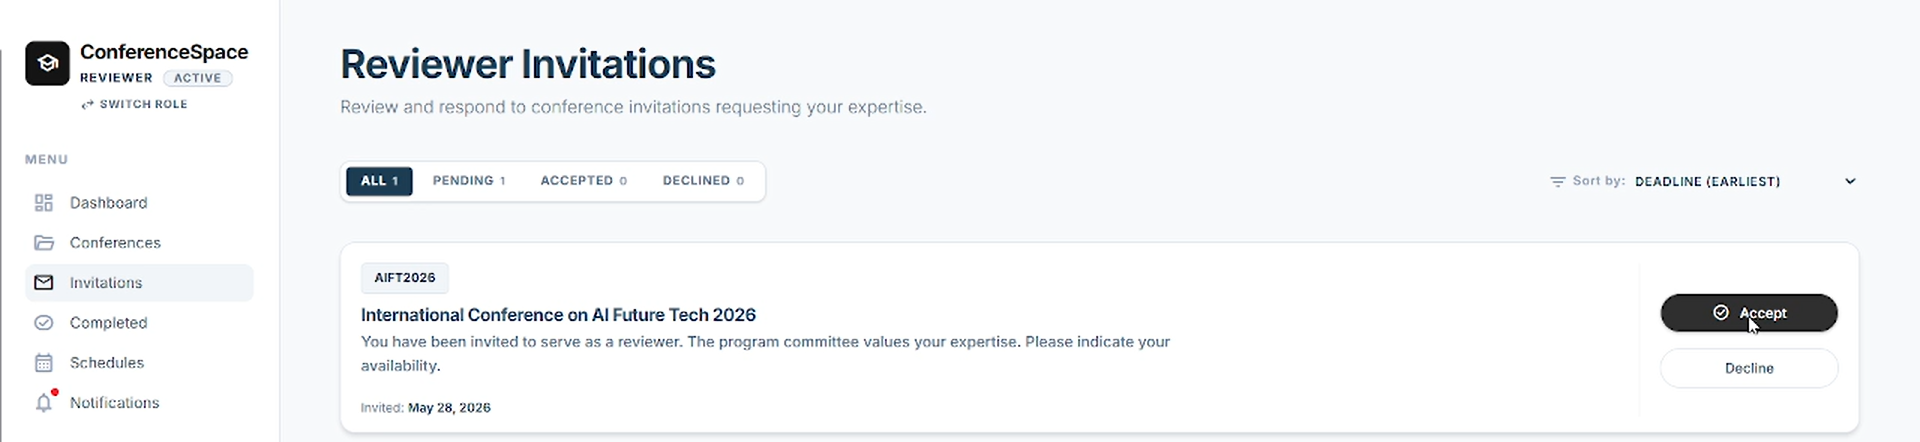
\includegraphics[width=0.95\textwidth]{images/chapter_3_uc04_reviewer_invitations_1.png} \\
    \vspace{0.2cm}
    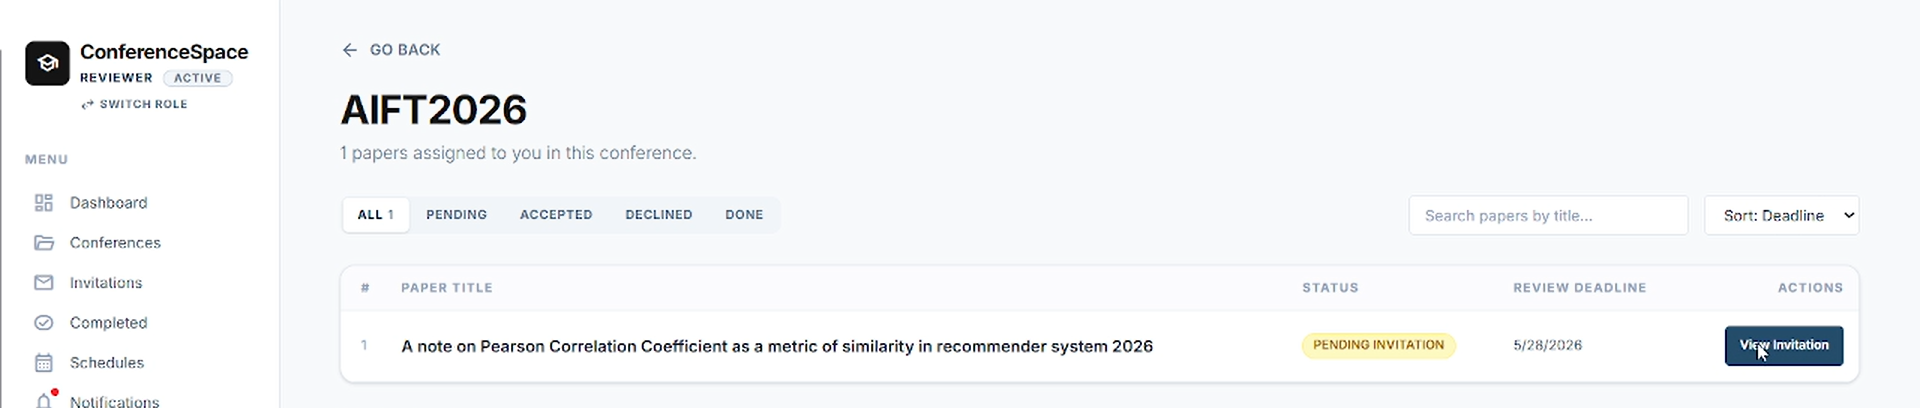
\includegraphics[width=0.95\textwidth]{images/chapter_3_uc04_reviewer_invitations_2.png}
  \end{tabular}
  \caption{Email thông báo lời mời (trên) và danh sách lời mời tham gia phản biện trong hệ thống (dưới)}
  \label{fig:uc04-invitations-cut}
\end{figure}

Hình~\ref{fig:uc04-invitations-cut} minh họa giao diện tiếp nhận thông báo và danh sách lời mời tham gia phản biện hội nghị.

\begin{figure}[H]
  \centering
  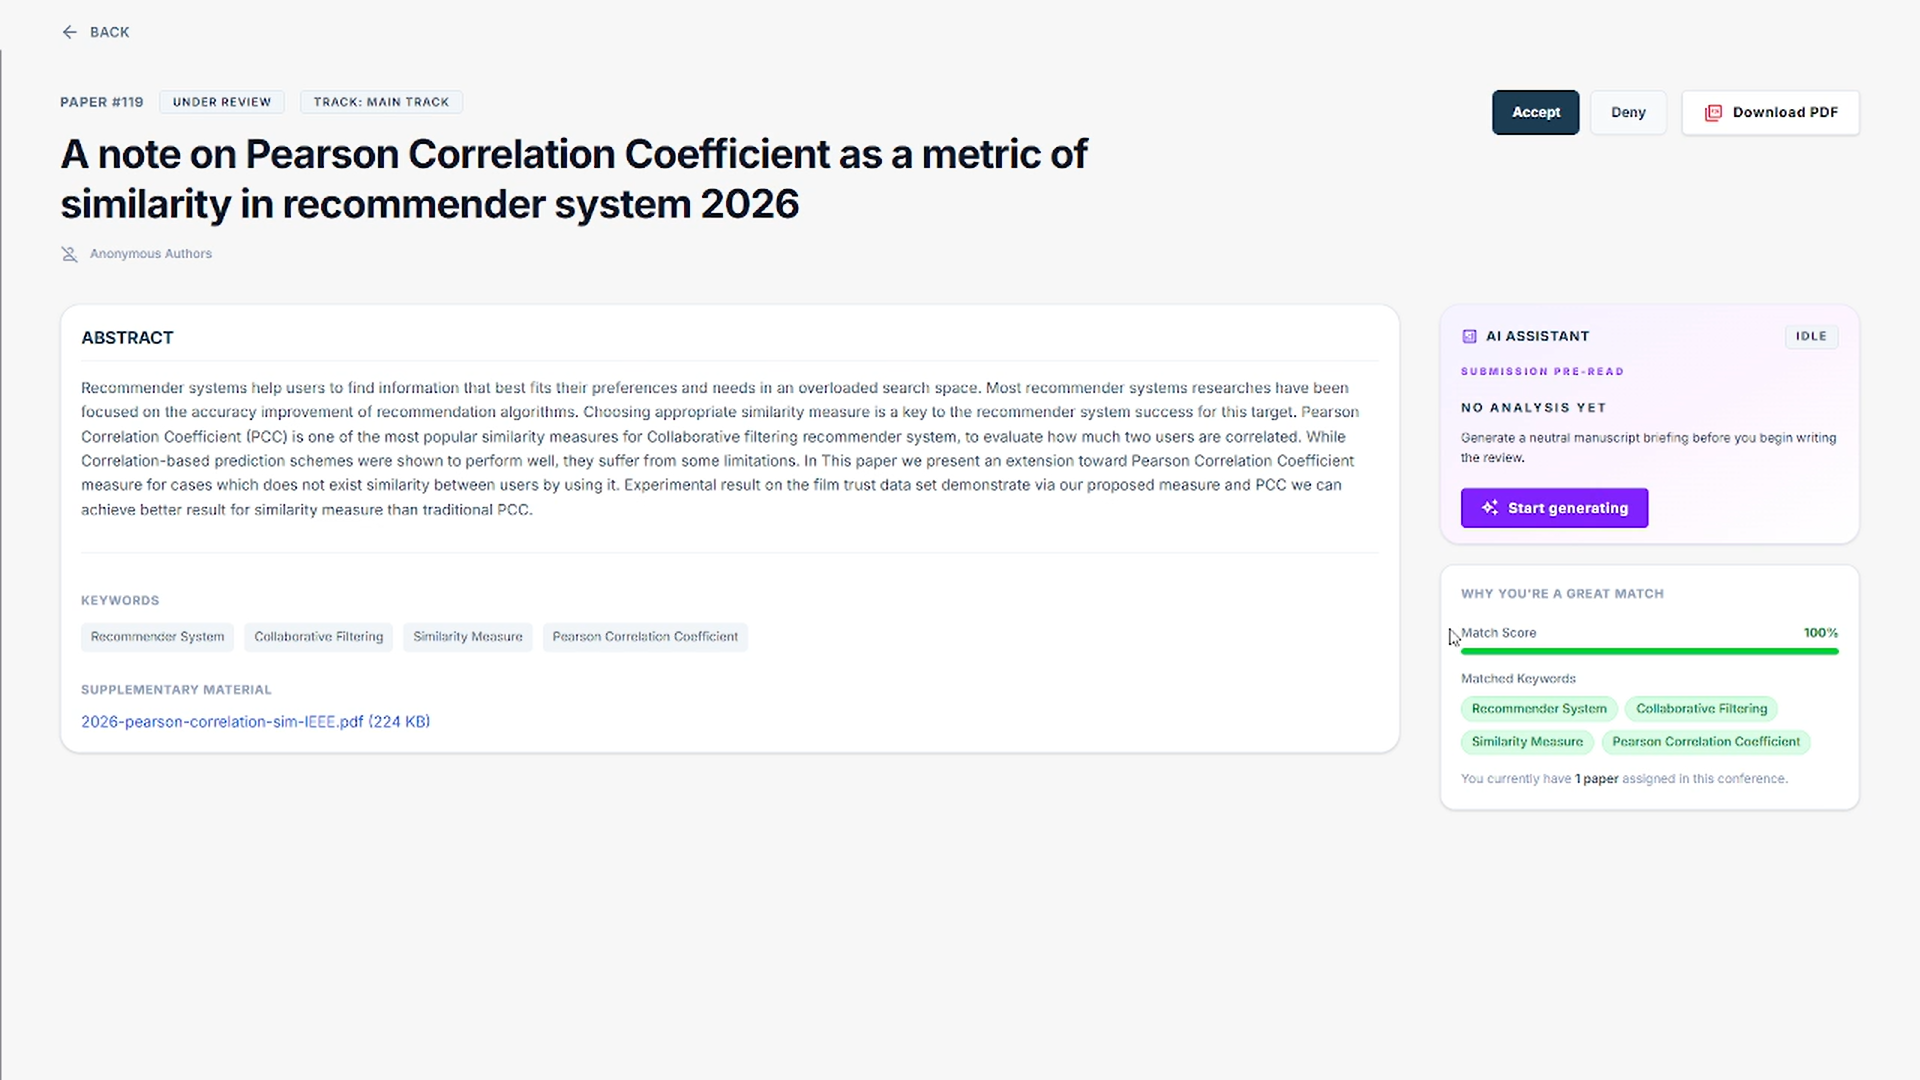
\includegraphics[width=0.95\textwidth]{images/chapter_3_uc04_accept_deny_assignment.png}
  \caption{Giao diện chi tiết bài nộp để Phản biện viên chấp nhận hoặc từ chối phân công}
  \label{fig:uc04-accept-deny-cut}
\end{figure}

Sau khi Chủ tọa tạo phân công, Phản biện viên dùng giao diện tại Hình~\ref{fig:uc04-accept-deny-cut} để xem bài nộp và chấp nhận hoặc từ chối phân công.

\subsubsection{UC-05. Đọc, soạn và gửi phản biện có AI hỗ trợ}

Phản biện viên mở bài được phân công, đọc bản thảo và nhập điểm, nhận xét, khuyến nghị cùng mức độ tự tin. Reviewer Initial Analysis có thể cung cấp bản định hướng ban đầu, nhưng Phản biện viên phải đối chiếu nội dung này với bài gốc và tự hình thành nhận định. Trước khi gửi, Review Quality Auditor rà soát mức độ đầy đủ, cụ thể và nhất quán của bản nháp. Phản biện viên xem các phát hiện, chỉnh sửa khi cần và xác nhận gửi phản biện.

\begin{figure}[H]
  \centering
  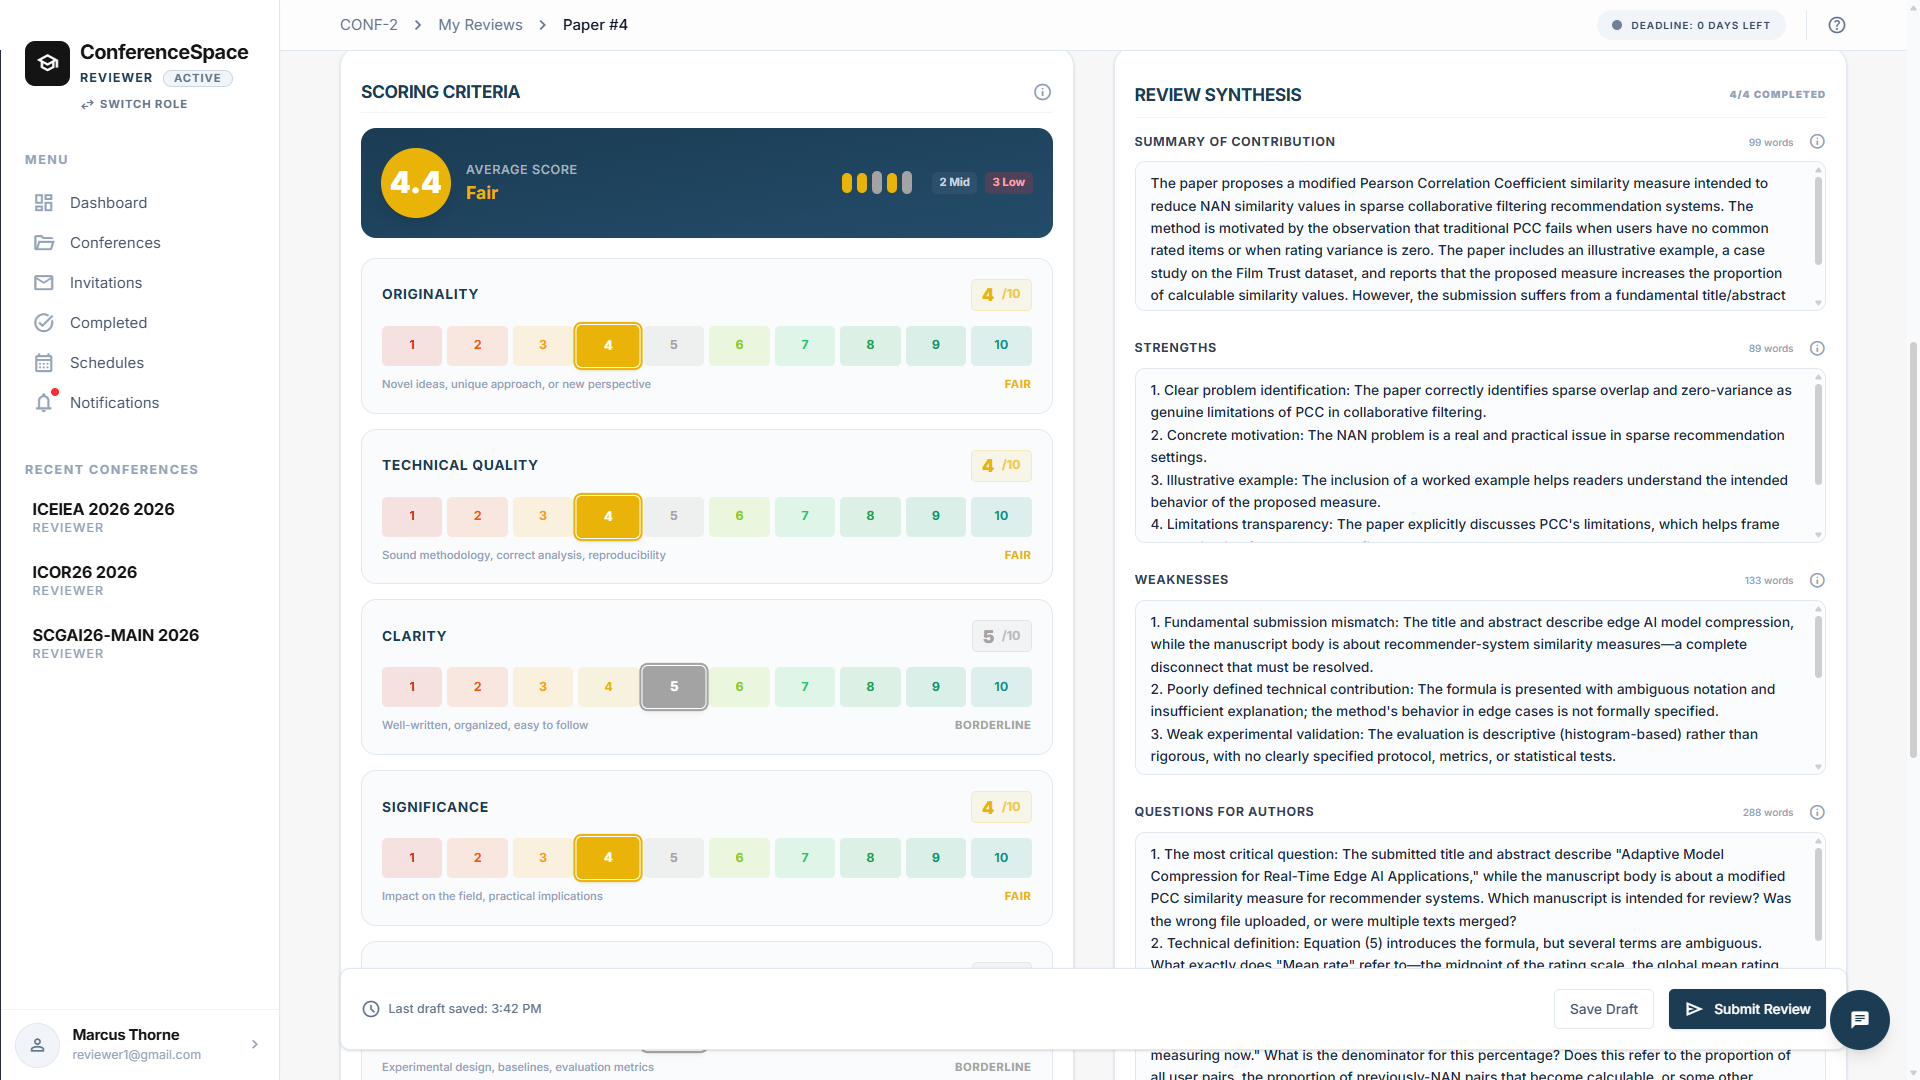
\includegraphics[width=0.95\textwidth]{images/chapter_3_uc05_reviewer_workspace_1.png}
  \caption{Không gian đọc bài và soạn phản biện của Phản biện viên}
  \label{fig:uc05-workspace-cut}
\end{figure}

Hình~\ref{fig:uc05-workspace-cut} đặt hai chức năng AI vào đúng bối cảnh sử dụng: chúng hỗ trợ một quy trình mà Phản biện viên vẫn phải đọc bản thảo, nhập nhận xét và chịu trách nhiệm về bản phản biện cuối cùng.

\begin{figure}[H]
  \centering
  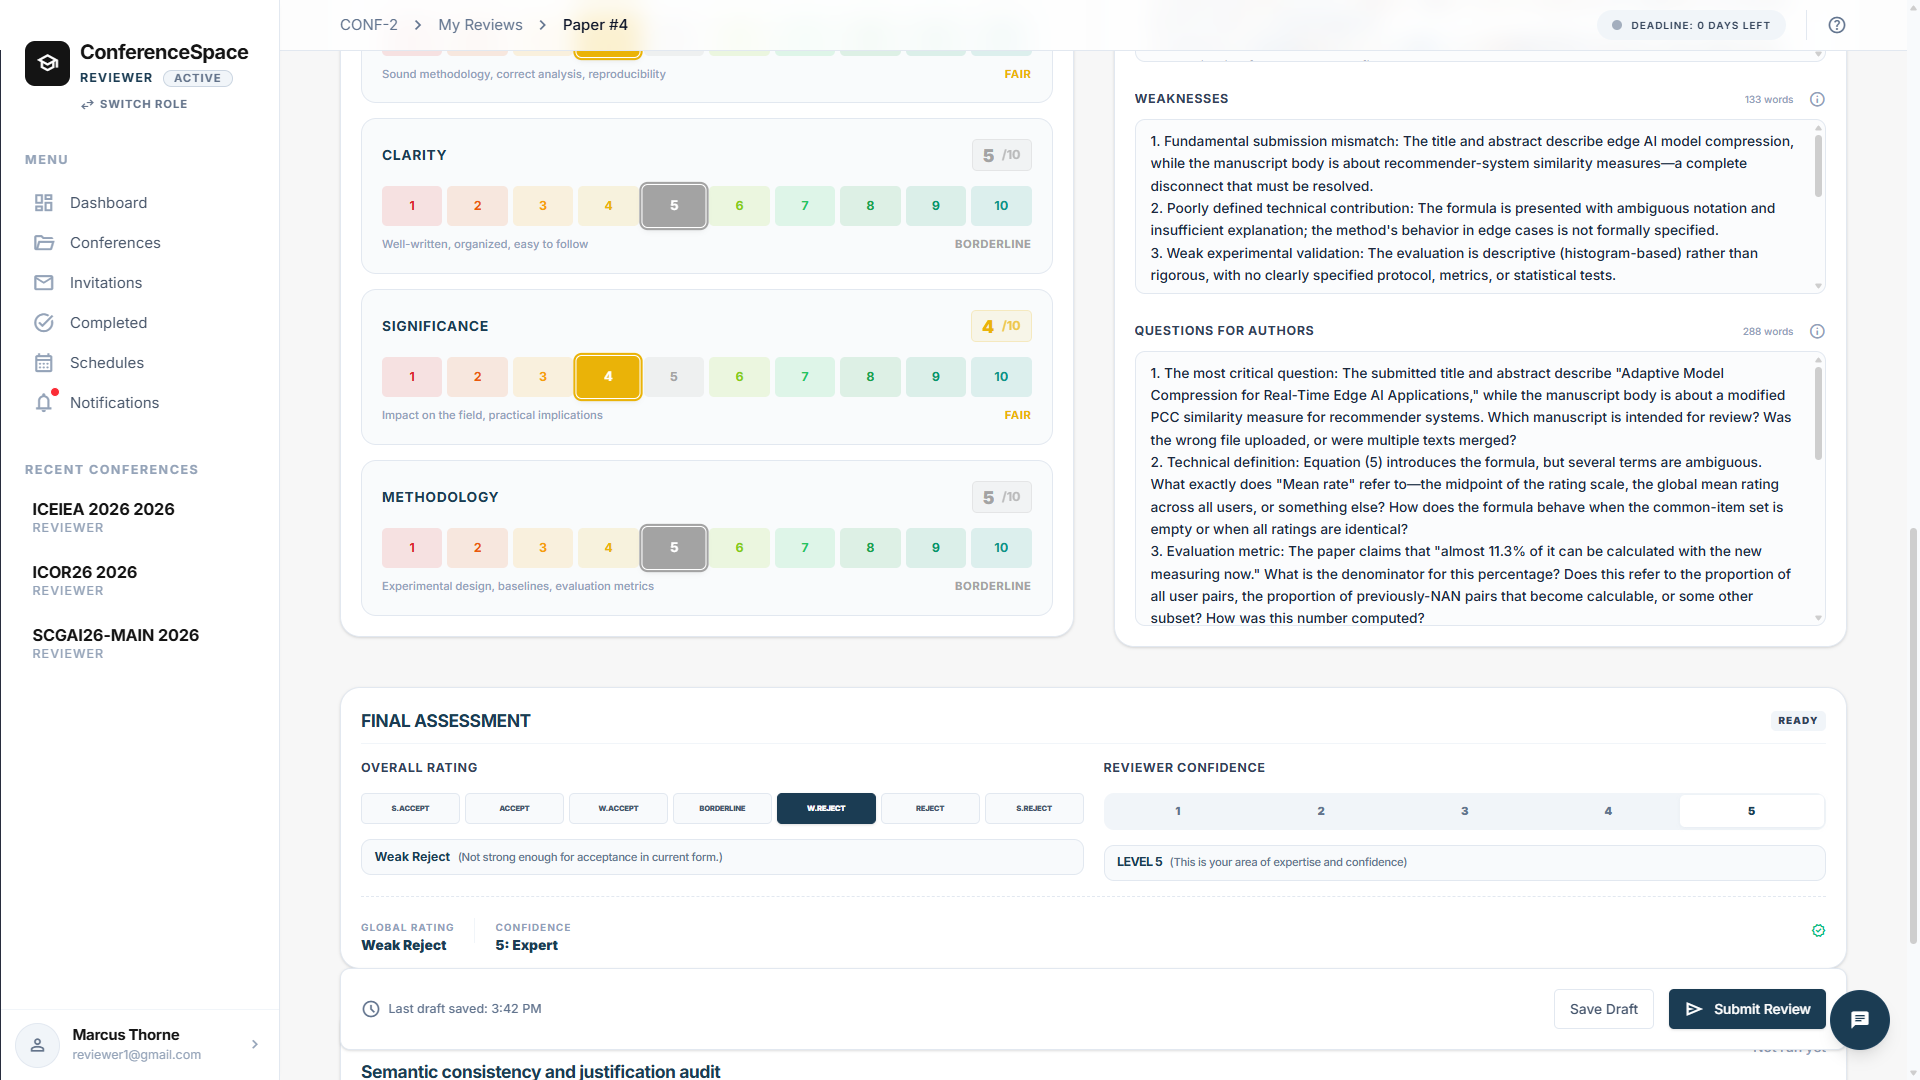
\includegraphics[width=0.95\textwidth]{images/chapter_3_uc05_reviewer_workspace_2.png}
  \caption{Không gian làm việc với biểu mẫu phản biện mở rộng của Phản biện viên}
  \label{fig:uc05-workspace-2-cut}
\end{figure}

Hình~\ref{fig:uc05-workspace-2-cut} trình bày một biến thể khác của không gian làm việc và biểu mẫu phản biện.

\begin{figure}[H]
  \centering
  \makebox[\textwidth][c]{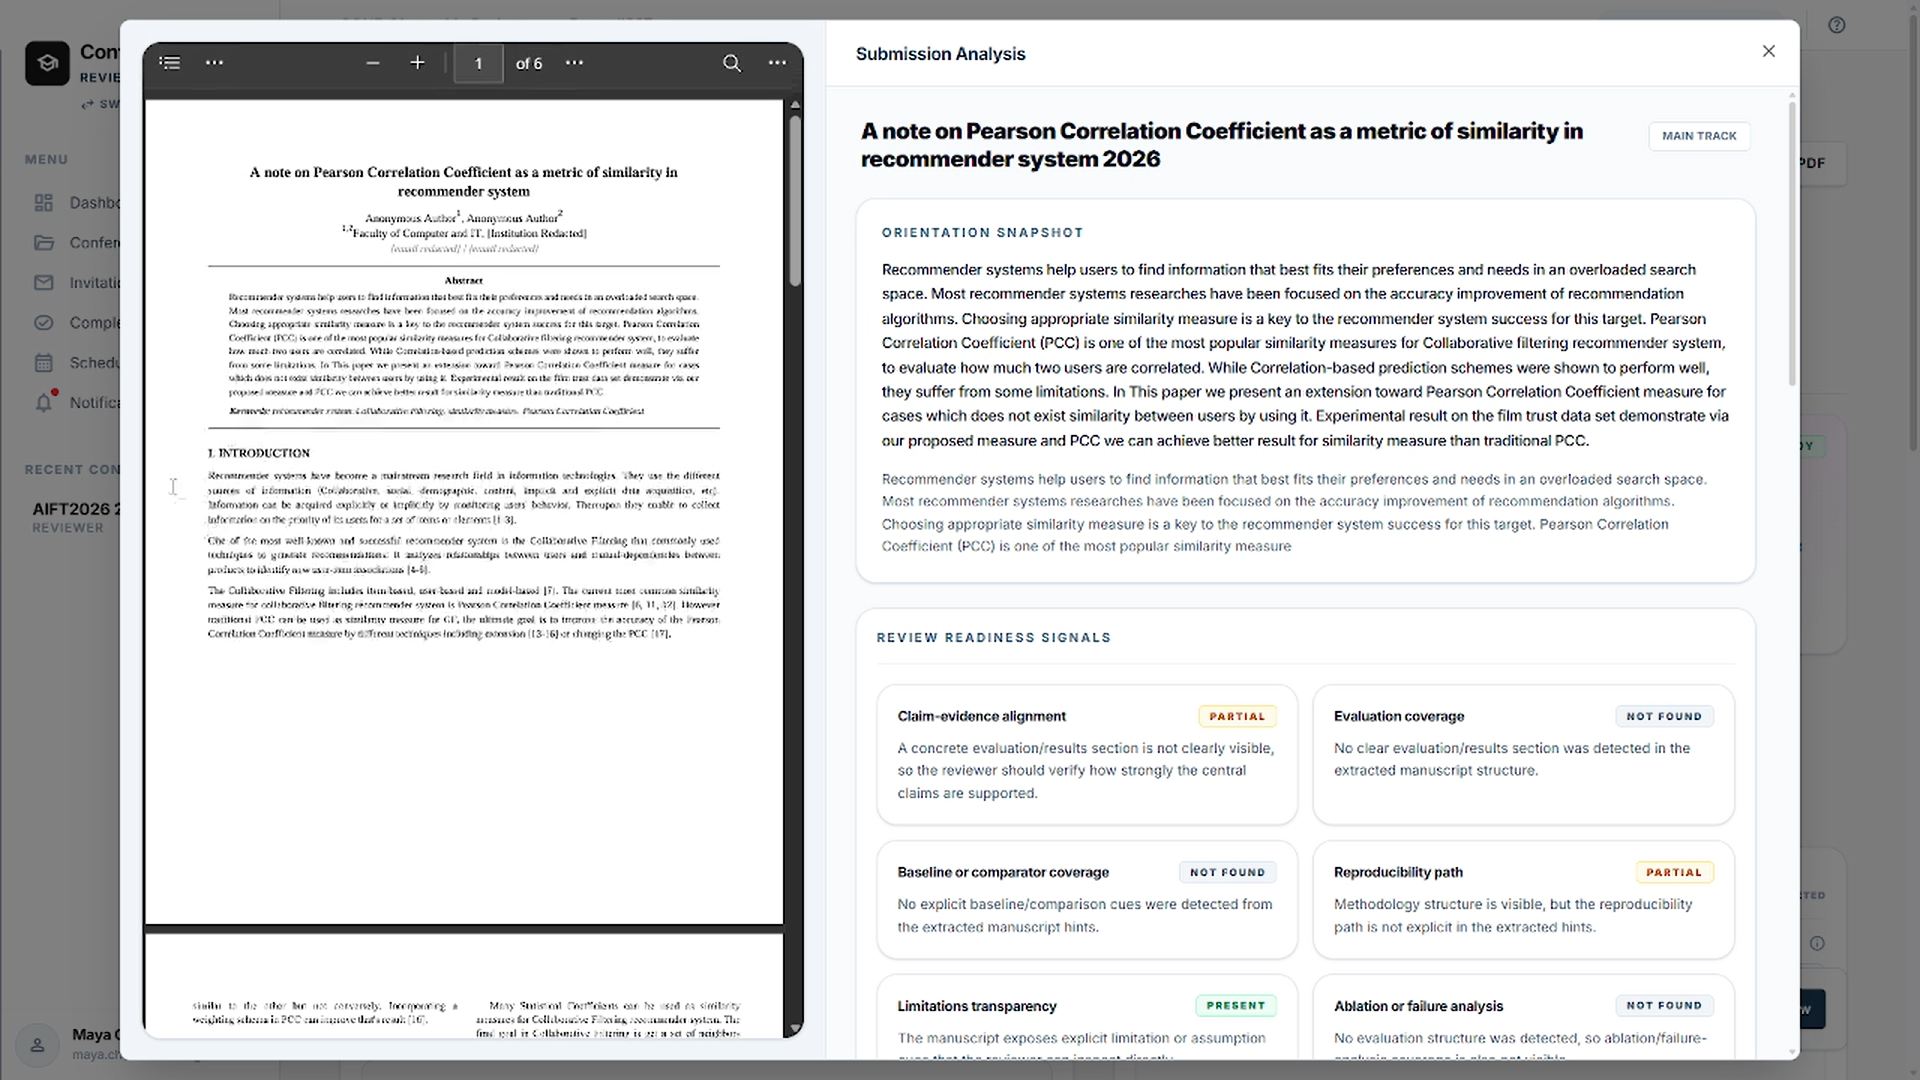
\includegraphics[width=1.10\textwidth]{images/chapter_3_uc05_reviewer_initial_analysis.png}}
  \caption{Bản định hướng đọc của Reviewer Initial Analysis}
  \label{fig:uc05-ria-cut}
\end{figure}

Hình~\ref{fig:uc05-ria-cut} thể hiện bản định hướng đọc do Reviewer Initial Analysis tạo ra để Phản biện viên tham khảo trước khi bắt đầu soạn phản biện.

\begin{figure}[H]
  \centering
  \makebox[\textwidth][c]{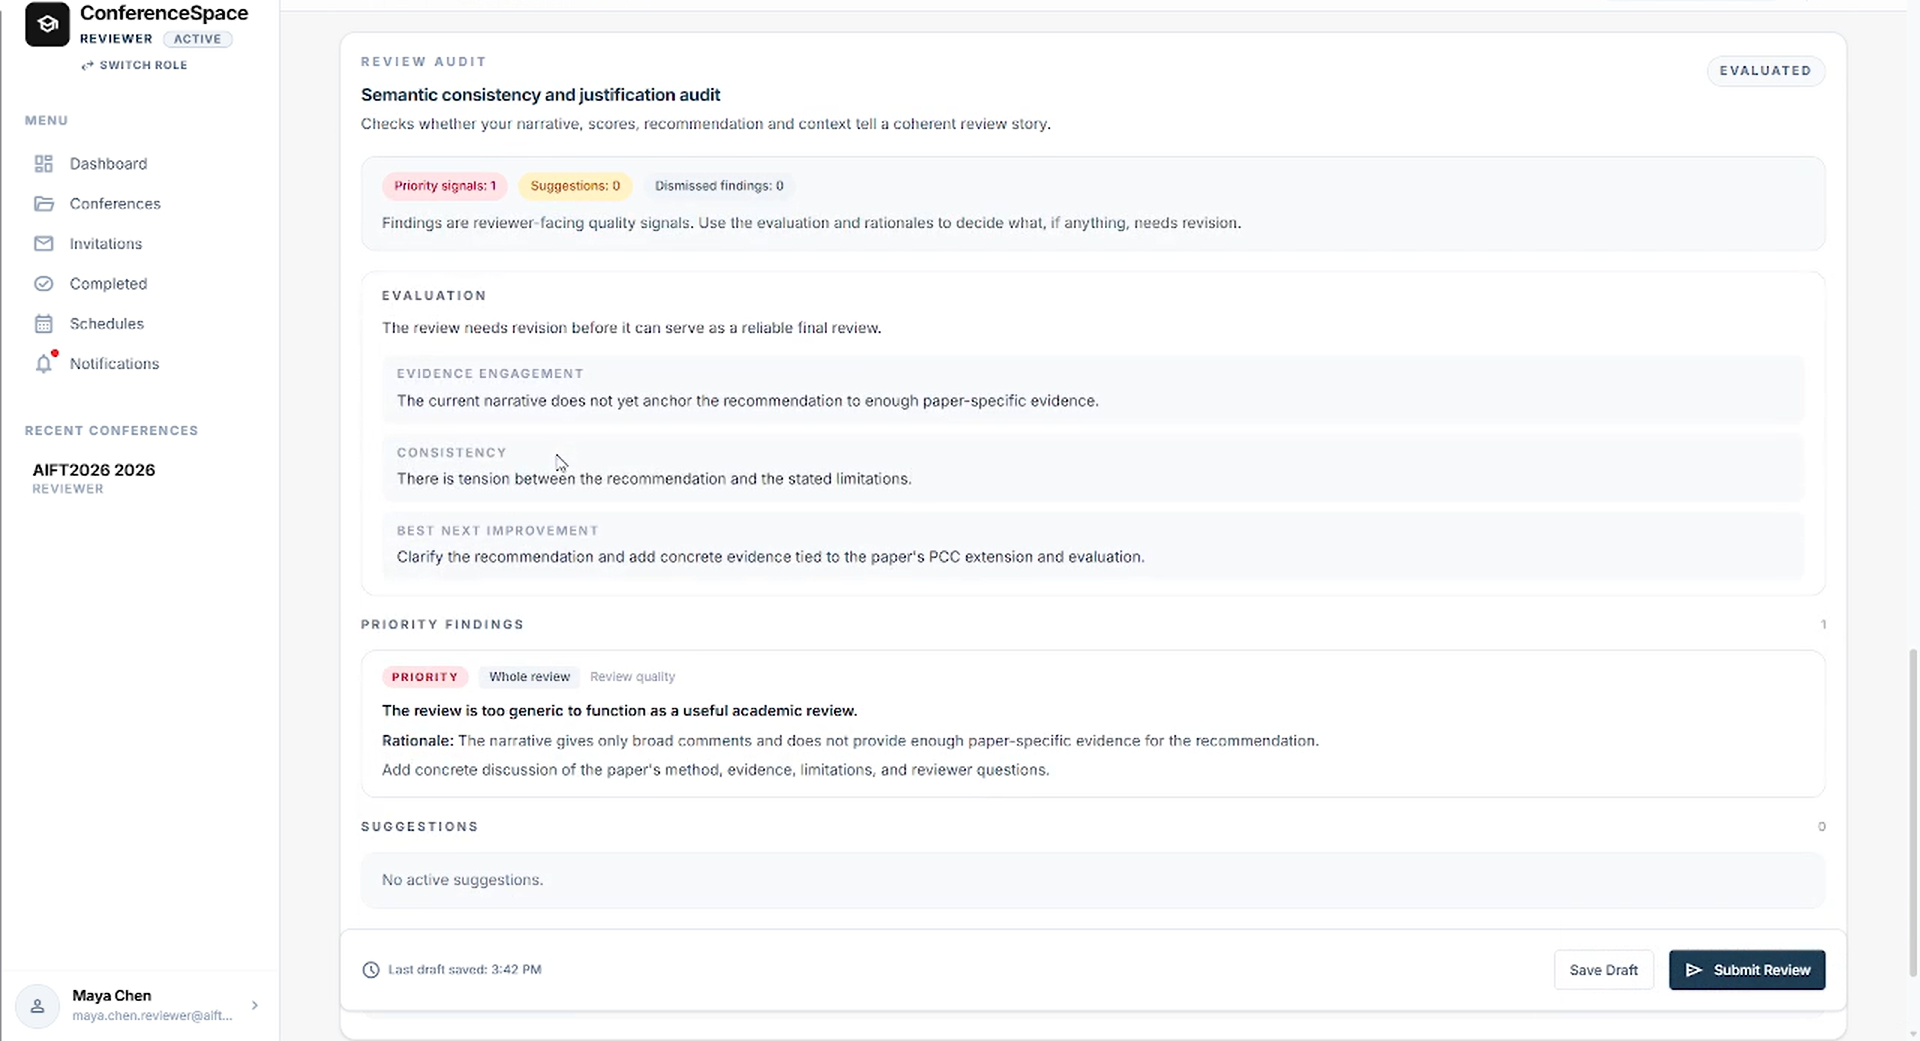
\includegraphics[width=1.10\textwidth]{images/chapter_3_uc05_reviewer_quality_auditor.png}}
  \caption{Bảng rà soát bản nháp của Review Quality Auditor}
  \label{fig:uc05-rqa-cut}
\end{figure}

Trước khi gửi phản biện, Phản biện viên xem bảng rà soát do Review Quality Auditor tạo ra tại Hình~\ref{fig:uc05-rqa-cut}.

Review Quality Auditor chạy trước khi gửi để đưa các phát hiện vào bảng rà soát. Phát hiện mức \textit{blocking} được làm nổi bật nhưng không ngăn Phản biện viên gửi phản biện. Nếu tác vụ rà soát không thể hoàn tất do lỗi dịch vụ, backend yêu cầu Phản biện viên xác nhận tiếp tục mà không có kết quả rà soát và ghi sự kiện này vào nhật ký. Hệ thống phân biệt phát hiện về chất lượng với lỗi không thể thực hiện bước rà soát: phát hiện chất lượng cung cấp thông tin để Phản biện viên xem xét, còn lỗi thực thi được thông báo rõ và ghi vào nhật ký.

\subsubsection{UC-06. Phân công phản biện có kiểm tra xung đột lợi ích}

Hệ thống chuẩn bị các cặp bài nộp--Phản biện viên, tính điểm phù hợp, loại các cặp có xung đột lợi ích khỏi đề xuất tự động và theo dõi số phân công được tạo trong cùng lượt chạy. Trước khi điều chỉnh hoặc xác nhận, Chủ tọa xem điểm số, lý do đối sánh, trạng thái kiểm tra xung đột lợi ích, tải phát sinh trong lượt chạy và danh sách bài chưa đủ Phản biện viên. Phản hồi \CodeBreak{AutoAssignResponse} không liệt kê đầy đủ từng cặp ứng viên bị loại. Khi Chủ tọa thêm đề xuất thủ công, backend kiểm tra quyền và trả cảnh báo xung đột lợi ích nhưng hiện chưa ngăn lưu; vì vậy, Chủ tọa phải xử lý cảnh báo trước khi xác nhận phương án.

\begin{figure}[H]
  \centering
  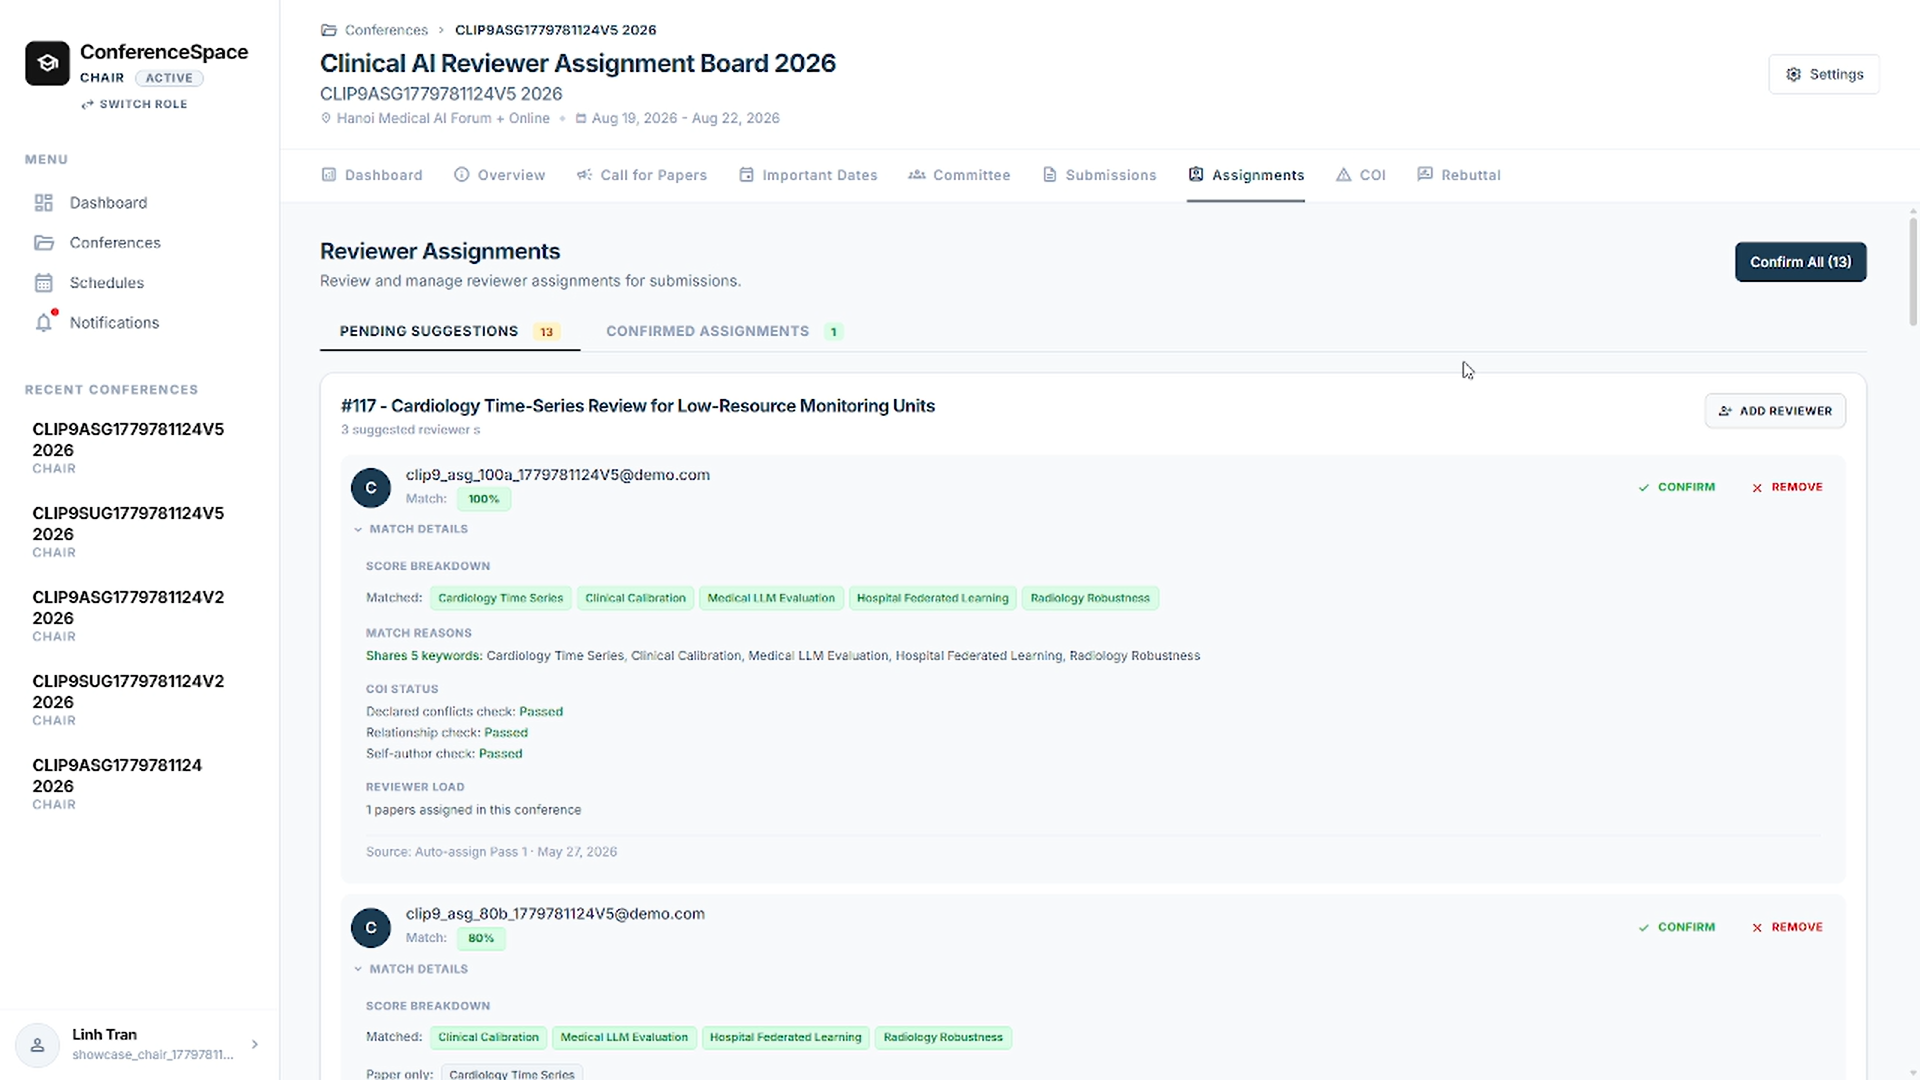
\includegraphics[width=0.95\textwidth]{images/chapter_3_uc06_assignment_dashboard.png}
  \caption{Giao diện bảng điều khiển quản lý phân công phản biện của Chủ tọa}
  \label{fig:uc06-dashboard-cut}
\end{figure}

Hình~\ref{fig:uc06-dashboard-cut} minh họa bảng điều khiển quản lý phân công phản biện của Chủ tọa.

\begin{figure}[H]
  \centering
  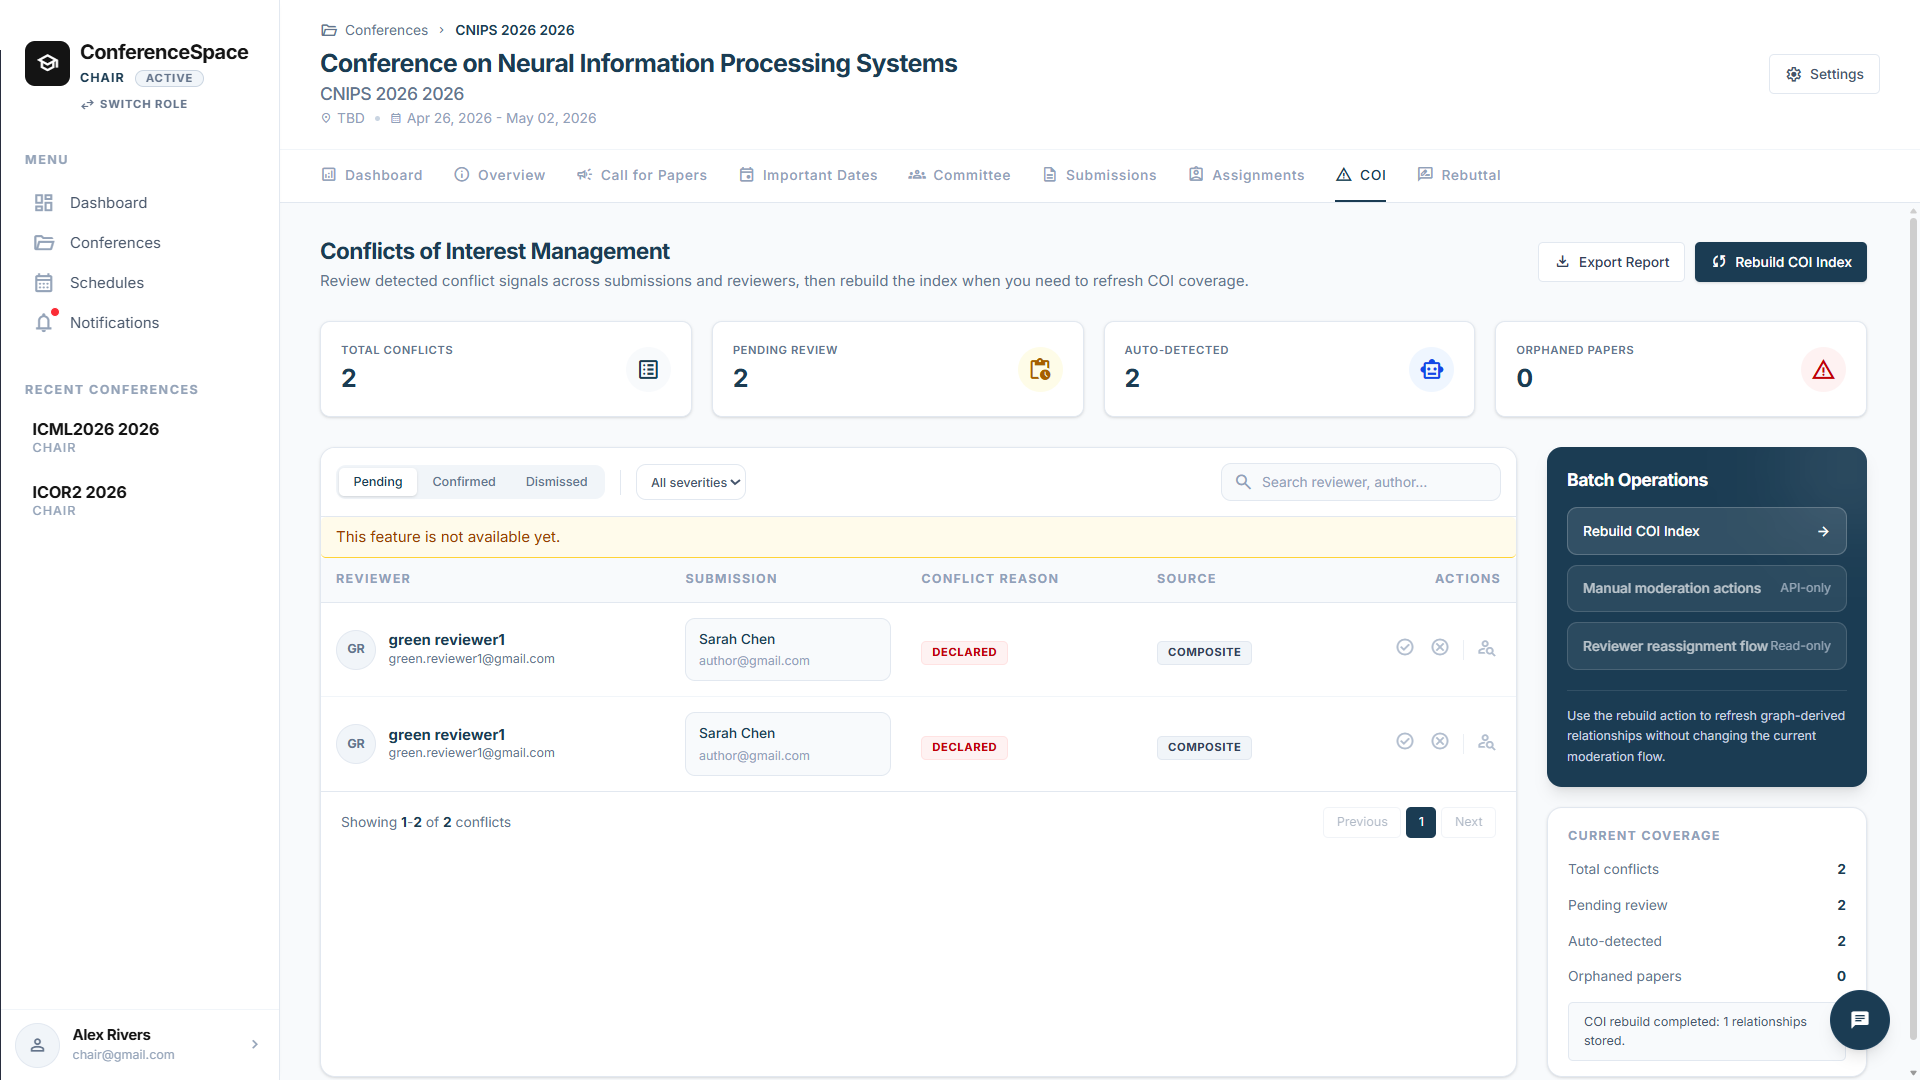
\includegraphics[width=0.95\textwidth]{images/chapter_3_uc06_coi_verification.png}
  \caption{Giao diện kiểm tra xung đột lợi ích giữa phản biện viên và bài nộp}
  \label{fig:uc06-coi-verification-cut}
\end{figure}

Hình~\ref{fig:uc06-coi-verification-cut} minh họa giao diện kiểm tra xung đột lợi ích giữa phản biện viên và bài nộp.

\begin{figure}[H]
  \centering
  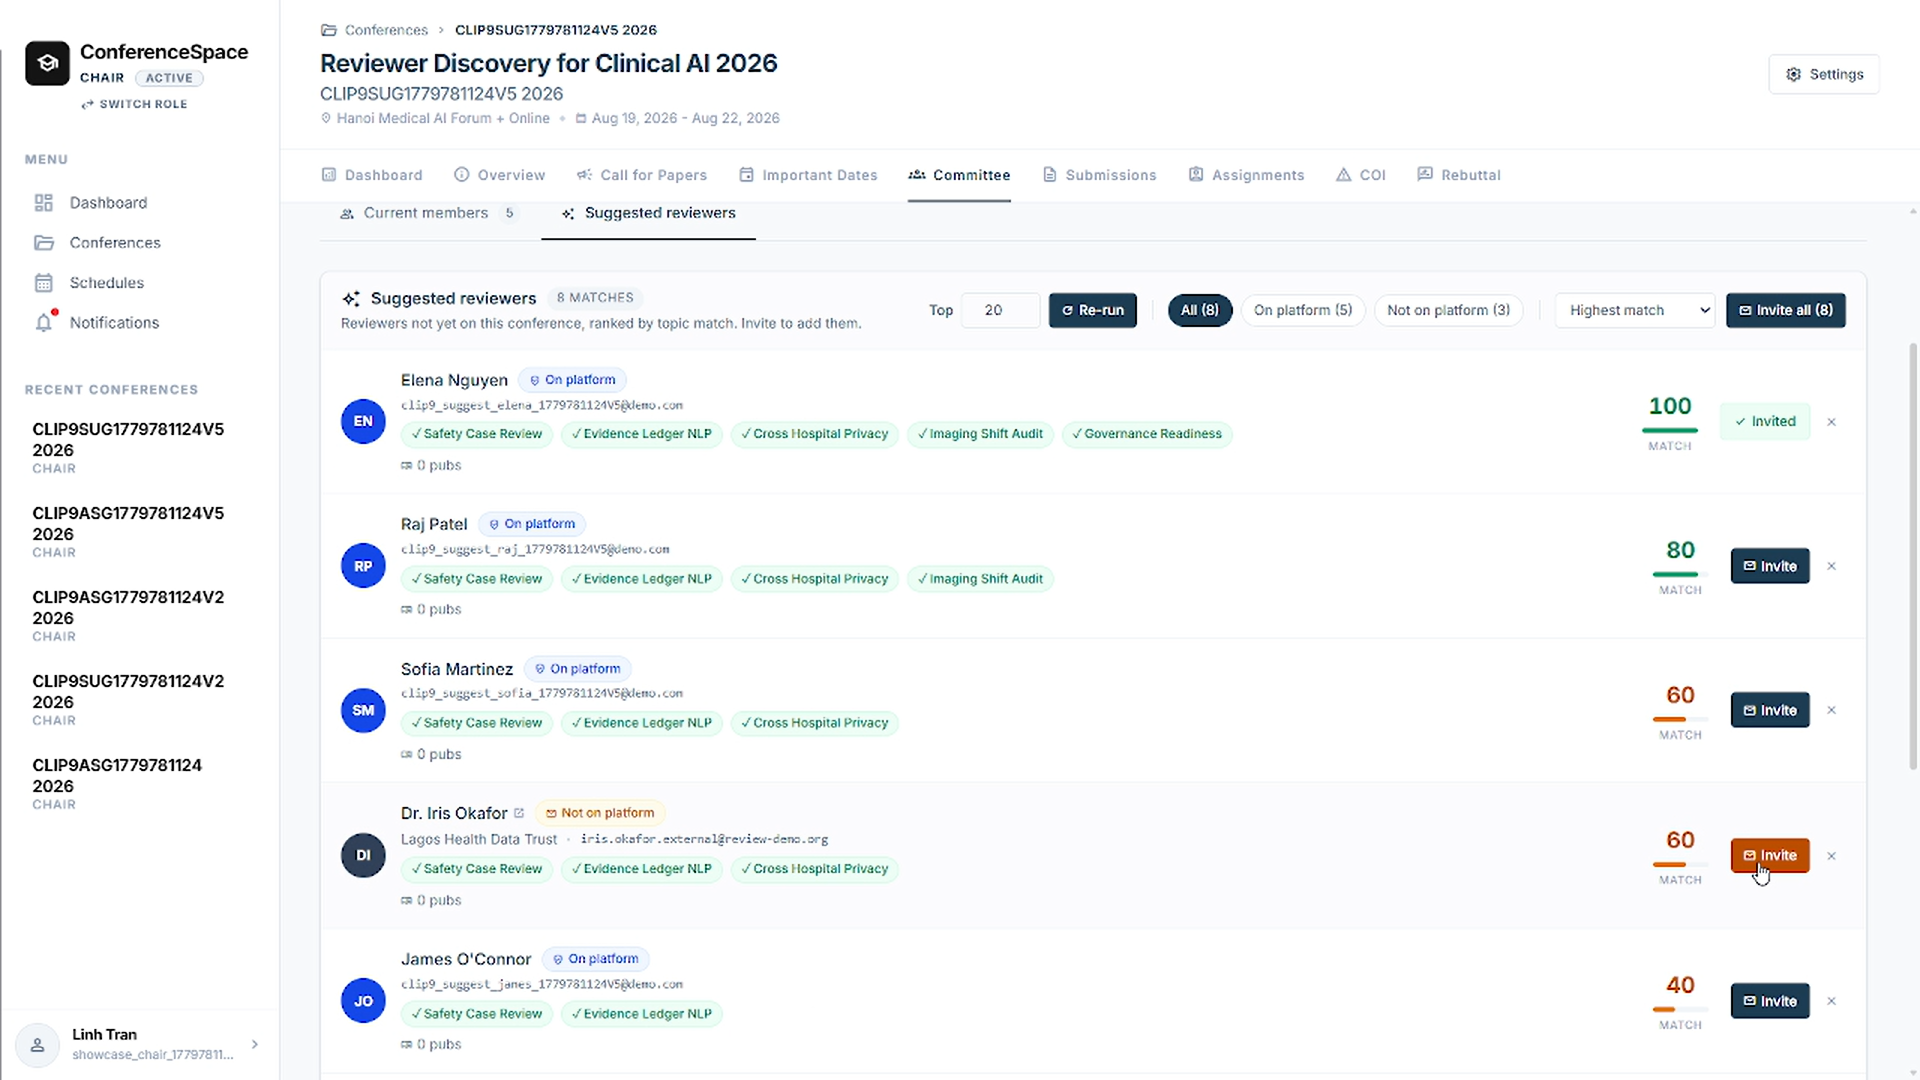
\includegraphics[width=0.95\textwidth]{images/chapter_3_uc06_assignment_suggestions.png}
  \caption{Danh sách đề xuất đối sánh và điểm phù hợp để Chủ tọa xem xét}
  \label{fig:uc06-suggestions-cut}
\end{figure}

Hình~\ref{fig:uc06-suggestions-cut} liệt kê các đề xuất đối sánh cùng điểm phù hợp để Chủ tọa xem xét trước khi xác nhận.

Công thức tính điểm, thủ tục phân công, lượt dự phòng và các trường hợp ngoại lệ được trình bày tại Mục~\ref{subsec:ch3-matching-cut}. Thuật toán tự động không nới ràng buộc xung đột lợi ích, kể cả khi hệ thống không tìm được đủ Phản biện viên; luồng thêm đề xuất thủ công hiện dùng cảnh báo thay cho cưỡng chế tại thời điểm ghi dữ liệu.

\subsubsection{UC-07. Quản lý hội nghị và theo dõi tiến độ}

Chủ tọa cấu hình thông tin hội nghị, chuyên đề, hạn chót nộp bài, biểu mẫu phản biện và chính sách; mời thành viên hội đồng chương trình; theo dõi số bài, tiến độ phản biện và các trường hợp cần xử lý. Hệ thống từ chối cấu hình thiếu trường bắt buộc, hạn chót nộp bài không hợp lệ hoặc thao tác của người dùng không có quyền. Bảng điều khiển hỗ trợ nhận biết các trường hợp cần xử lý nhưng không tự chuyển giai đoạn hoặc ra quyết định thay Chủ tọa.

\begin{figure}[H]
  \centering
  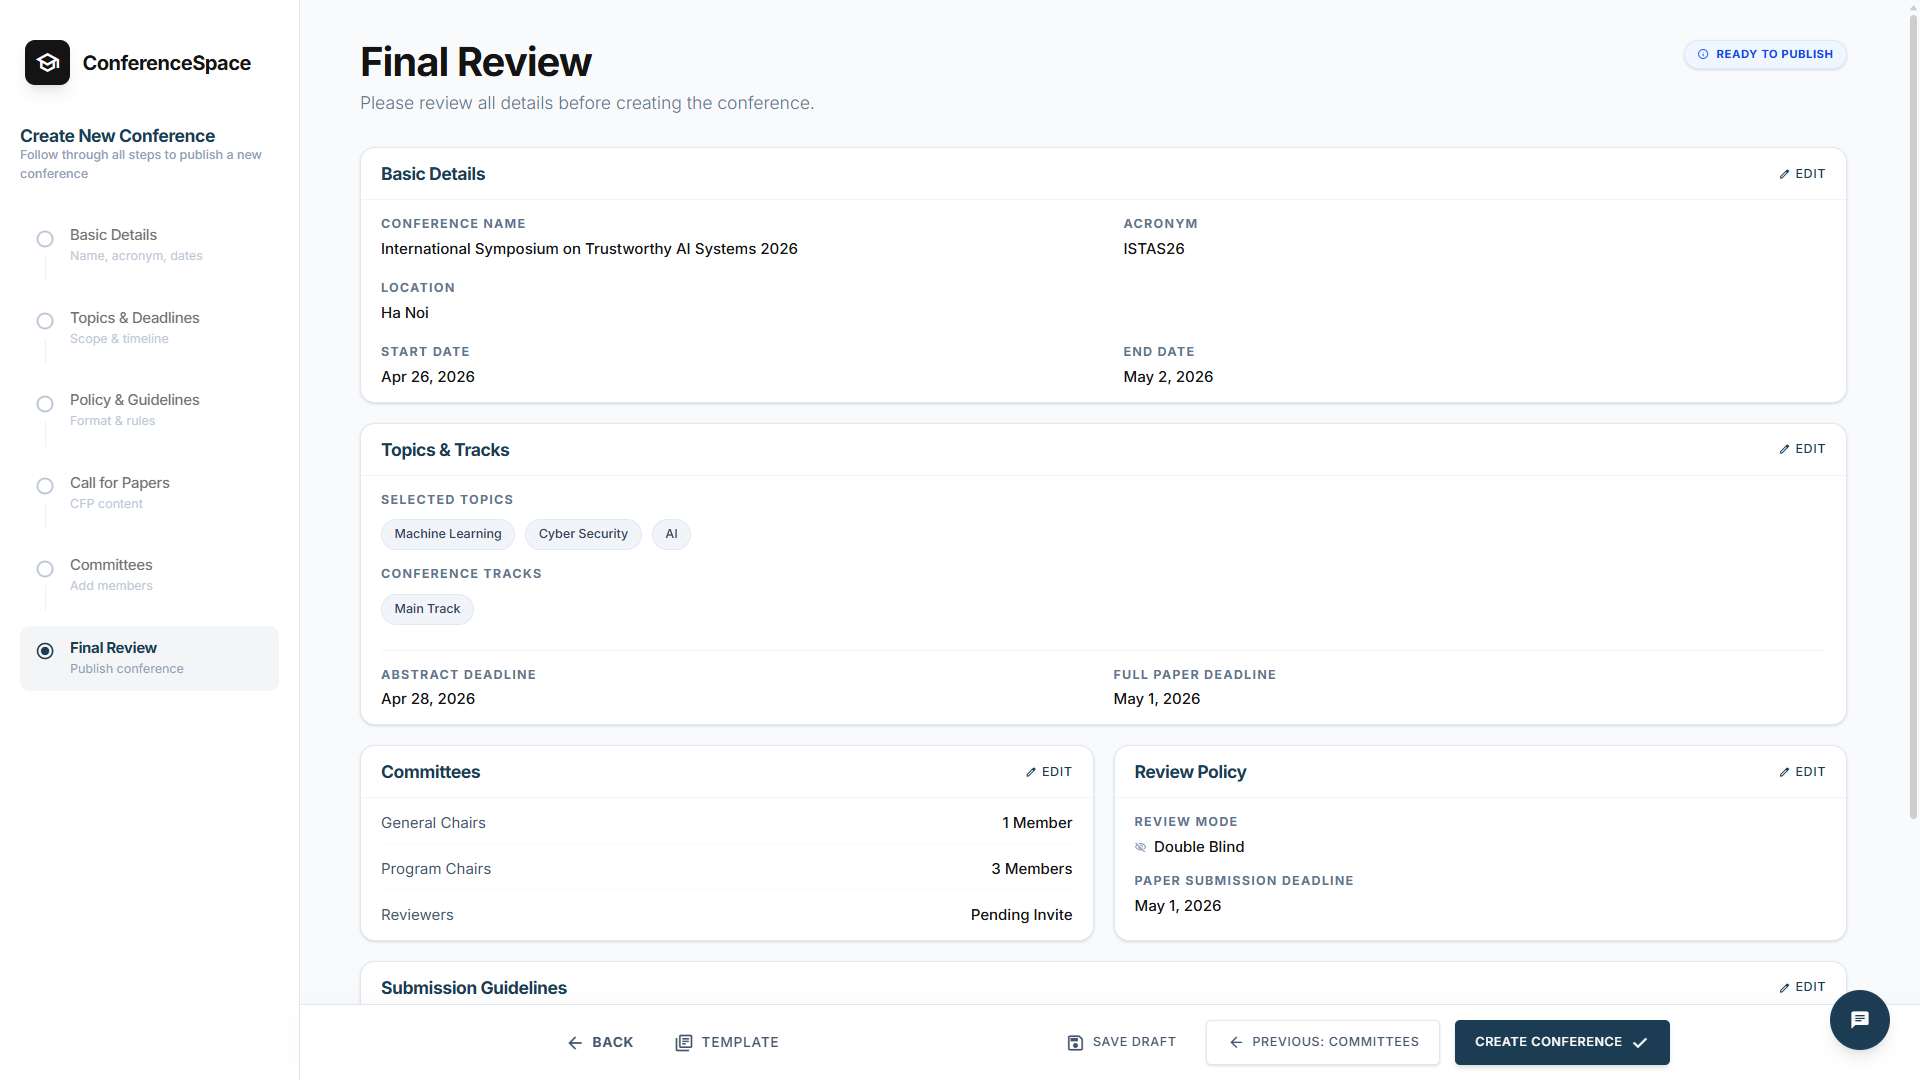
\includegraphics[width=0.95\textwidth]{images/chapter_3_uc07_conference_config.png}
  \caption{Giao diện thiết lập cấu hình thông tin và hạn chót nộp bài hội nghị của Chủ tọa}
  \label{fig:uc07-config-cut}
\end{figure}

Hình~\ref{fig:uc07-config-cut} thể hiện giao diện thiết lập cấu hình thông tin và hạn chót nộp bài hội nghị.

\begin{figure}[H]
  \centering
  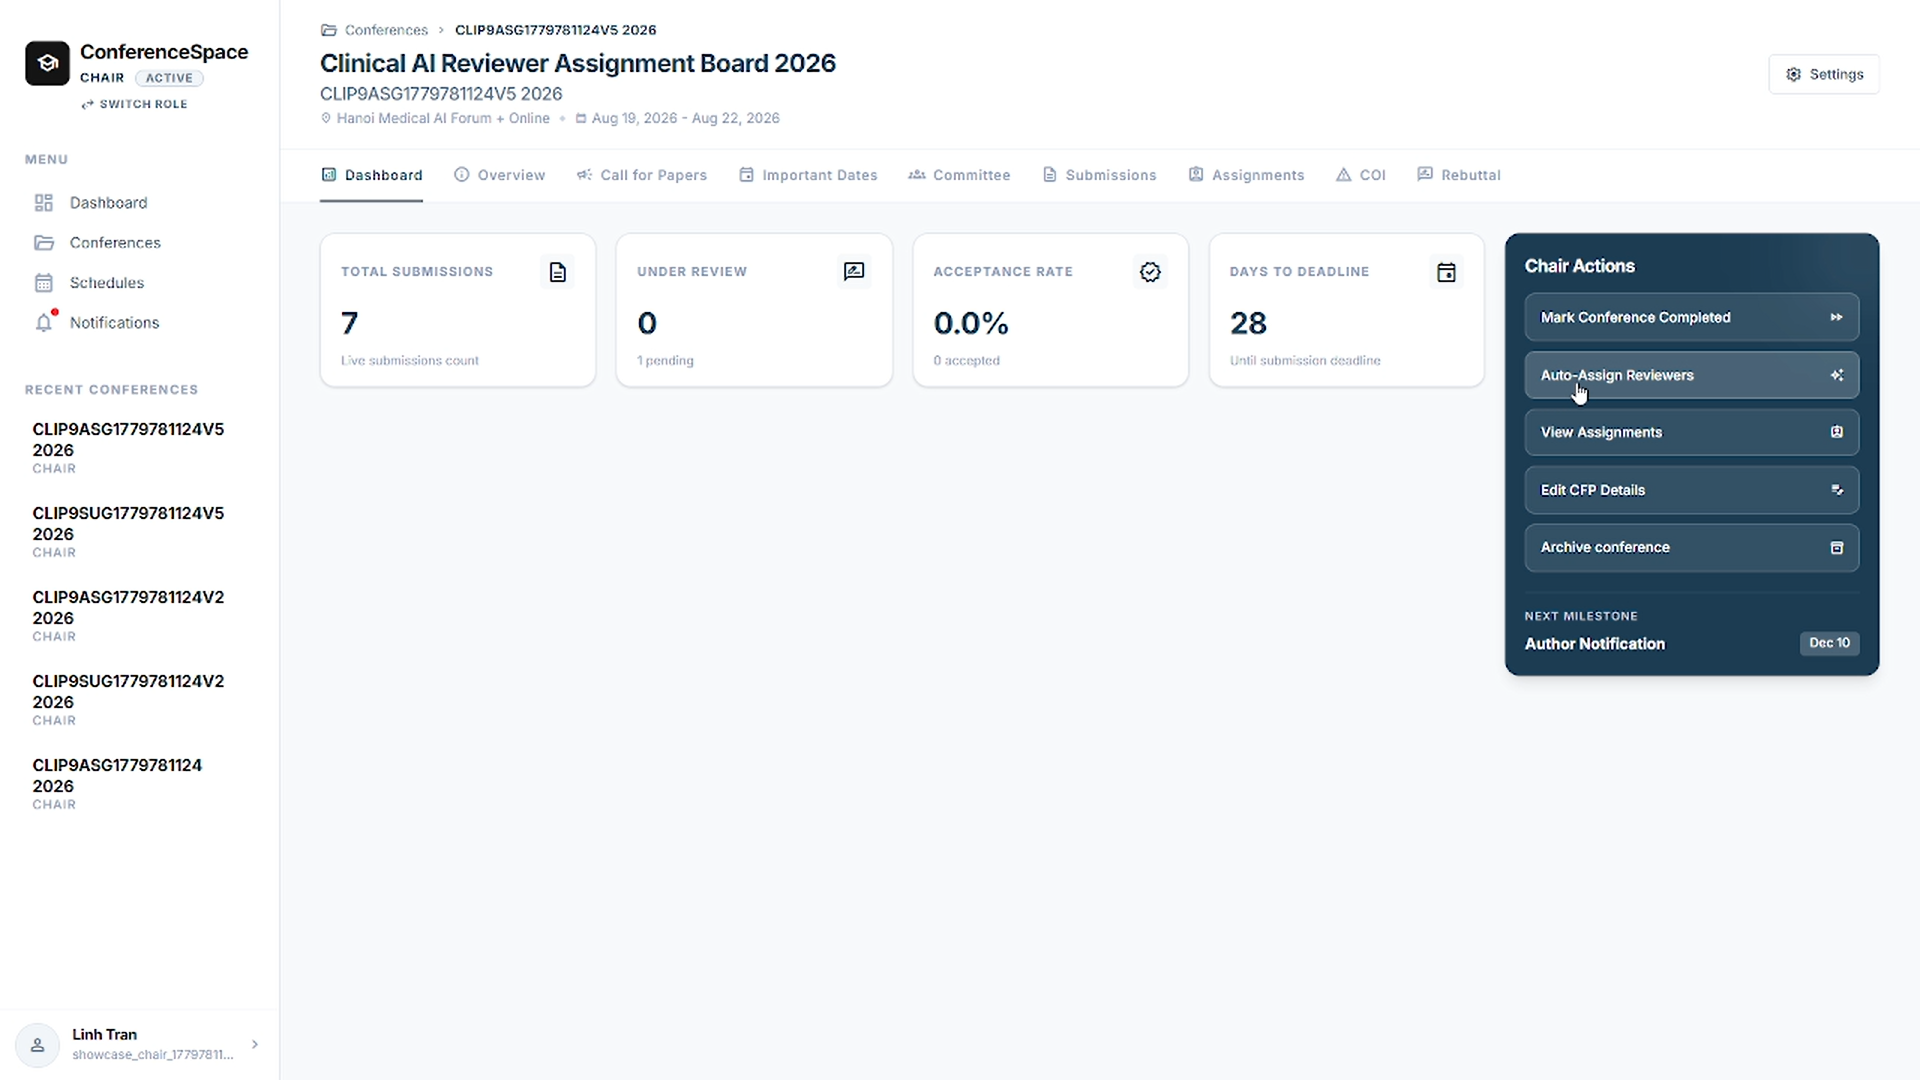
\includegraphics[width=0.95\textwidth]{images/chapter_3_uc07_chair_dashboard.png}
  \caption{Bảng điều khiển tiến độ hội nghị của Chủ tọa}
  \label{fig:uc07-dashboard-cut}
\end{figure}

Hình~\ref{fig:uc07-dashboard-cut} cung cấp cái nhìn tổng quan về hoạt động điều phối, bổ sung cho các hình chuyên biệt về đối sánh và hỗ trợ quyết định.

\begin{figure}[H]
  \centering
  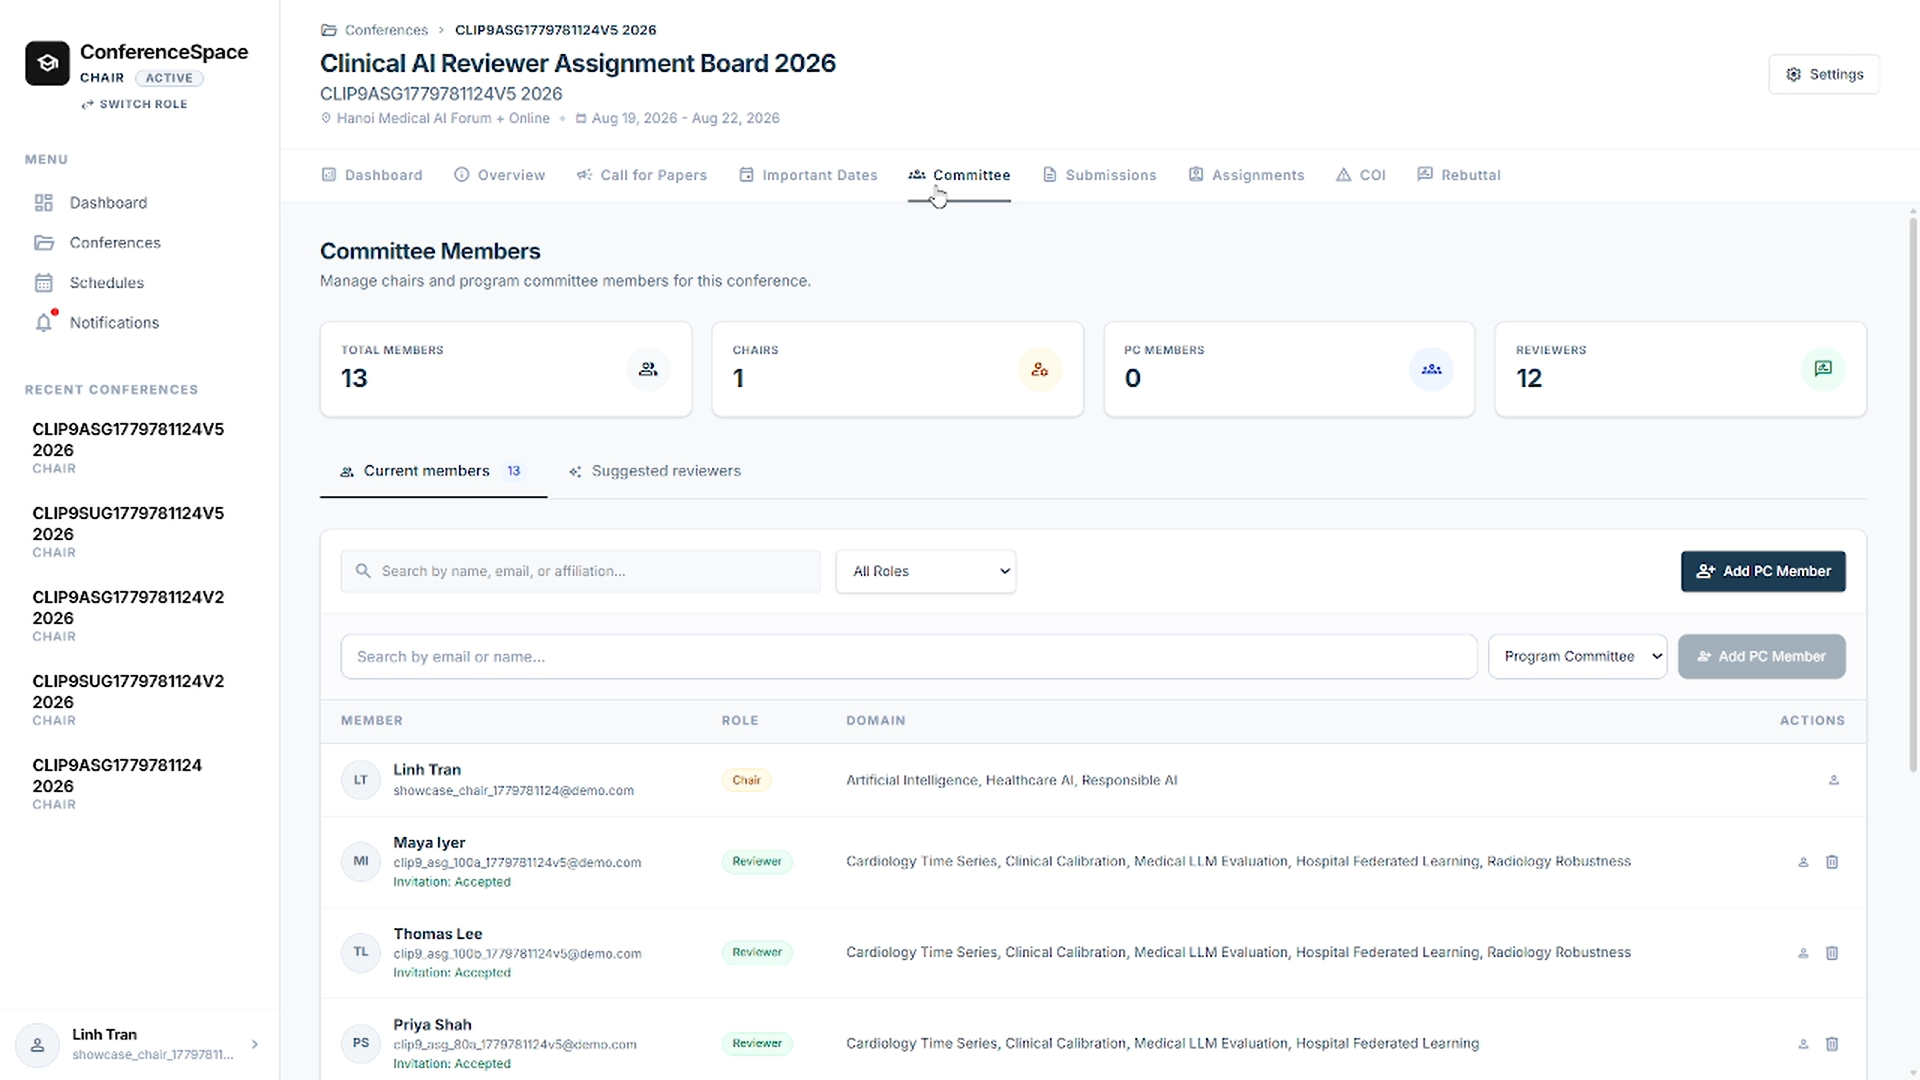
\includegraphics[width=0.95\textwidth]{images/chapter_3_uc07_committee_management.png}
  \caption{Giao diện quản lý ban chương trình và trạng thái lời mời phản biện viên}
  \label{fig:uc07-committee-cut}
\end{figure}

Hình~\ref{fig:uc07-committee-cut} minh họa giao diện quản lý ban chương trình và trạng thái lời mời phản biện viên.

\subsubsection{UC-08. Trao đổi theo bài nộp}

Chủ tọa hoặc Đồng chủ tọa mở giai đoạn phản hồi và kết thúc giai đoạn này trước khi ra quyết định; giai đoạn thảo luận chỉ được mở khi cấu hình hội nghị cho phép. Phản biện viên được phân công có thể tạo chuỗi thảo luận. Tác giả của bài và Phản biện viên trao đổi trong chuỗi tương ứng, còn Chủ tọa xem toàn bộ lịch sử ở chế độ giám sát. Sau khi đọc phản hồi, Phản biện viên có thể cập nhật điểm, khuyến nghị và nhận xét của bài mình phụ trách. Backend kiểm tra quan hệ giữa người dùng, bài nộp và chuỗi thảo luận trước mỗi thao tác. Nội dung trao đổi cùng đánh giá cập nhật được lưu với bài nộp và trở thành nguồn bằng chứng cho Chair Decision Copilot.

\begin{figure}[H]
  \centering
  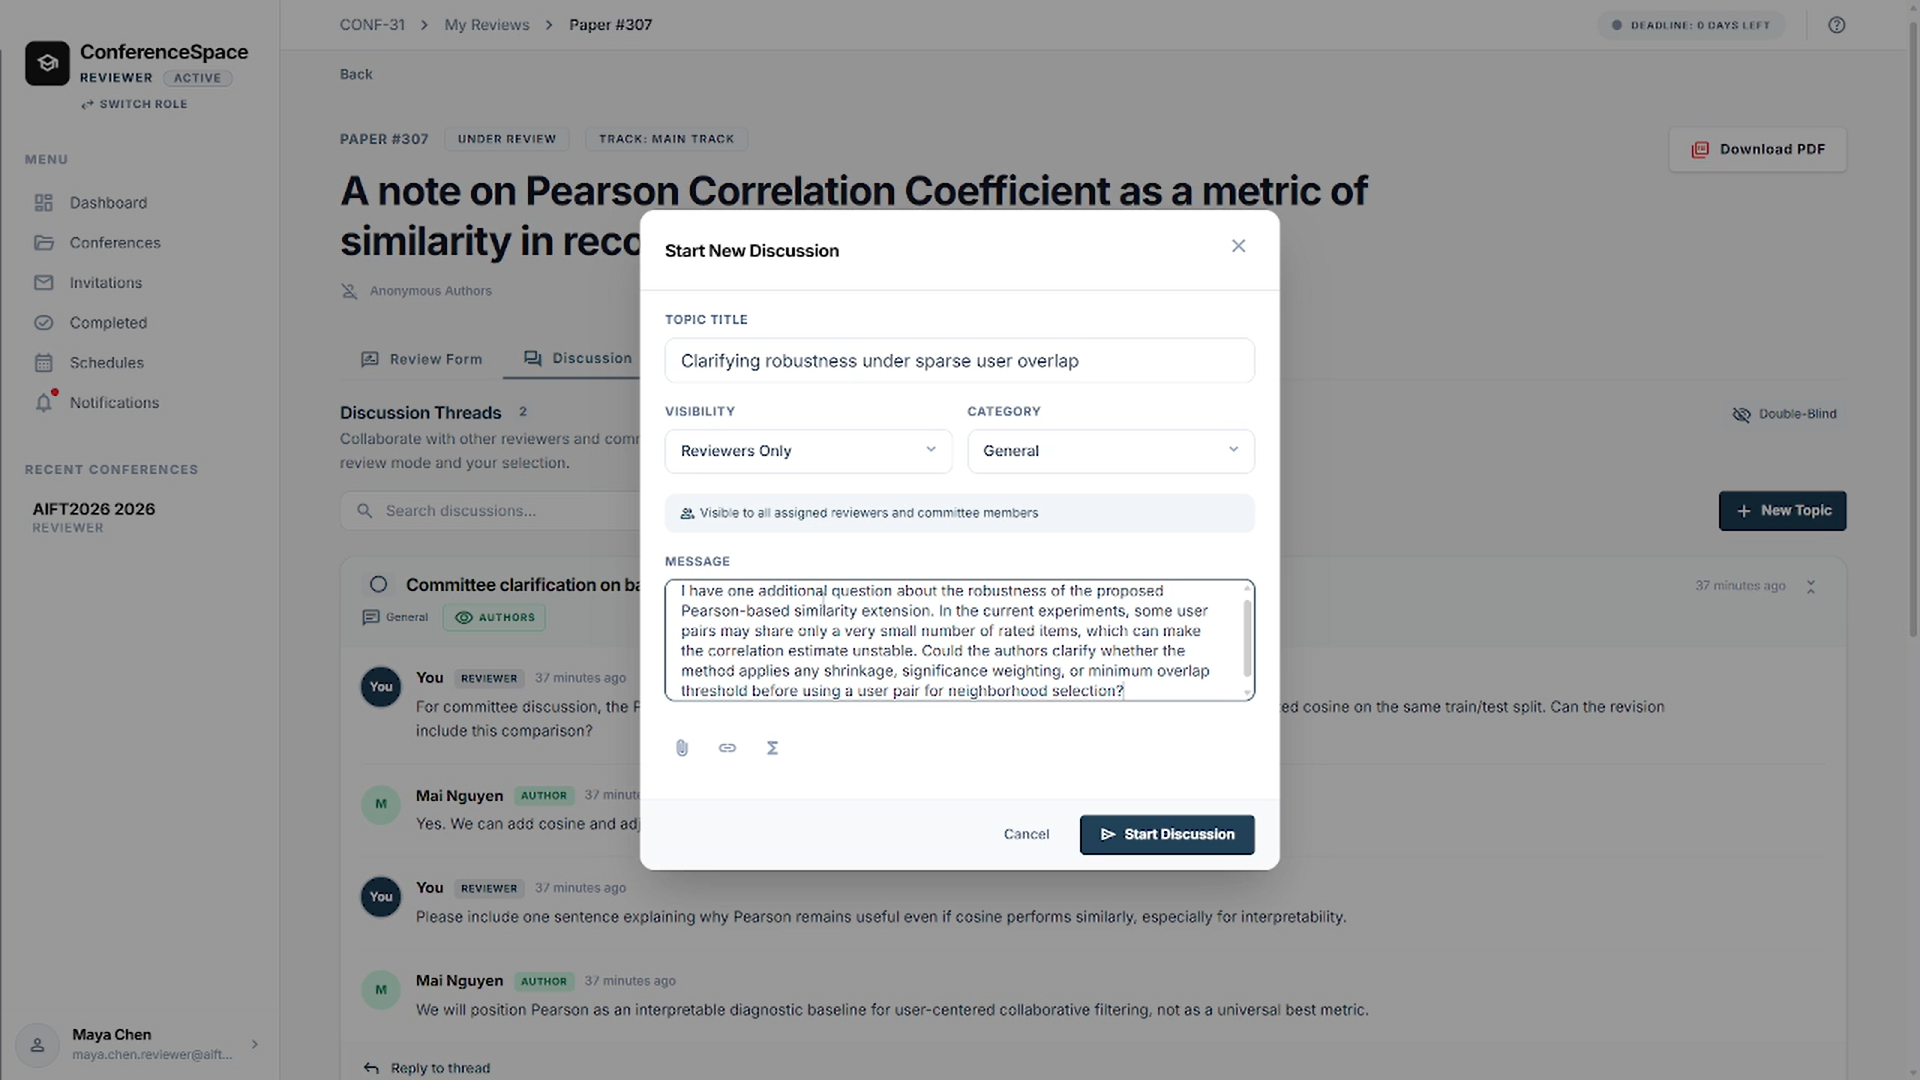
\includegraphics[width=0.95\textwidth]{images/chapter_3_uc08_create_discussion.png}
  \caption{Giao diện khởi tạo chủ đề thảo luận mới cho bài nộp}
  \label{fig:uc08-create-discussion-cut}
\end{figure}

Hình~\ref{fig:uc08-create-discussion-cut} minh họa giao diện khởi tạo chủ đề thảo luận mới cho bài nộp.

\begin{figure}[H]
  \centering
  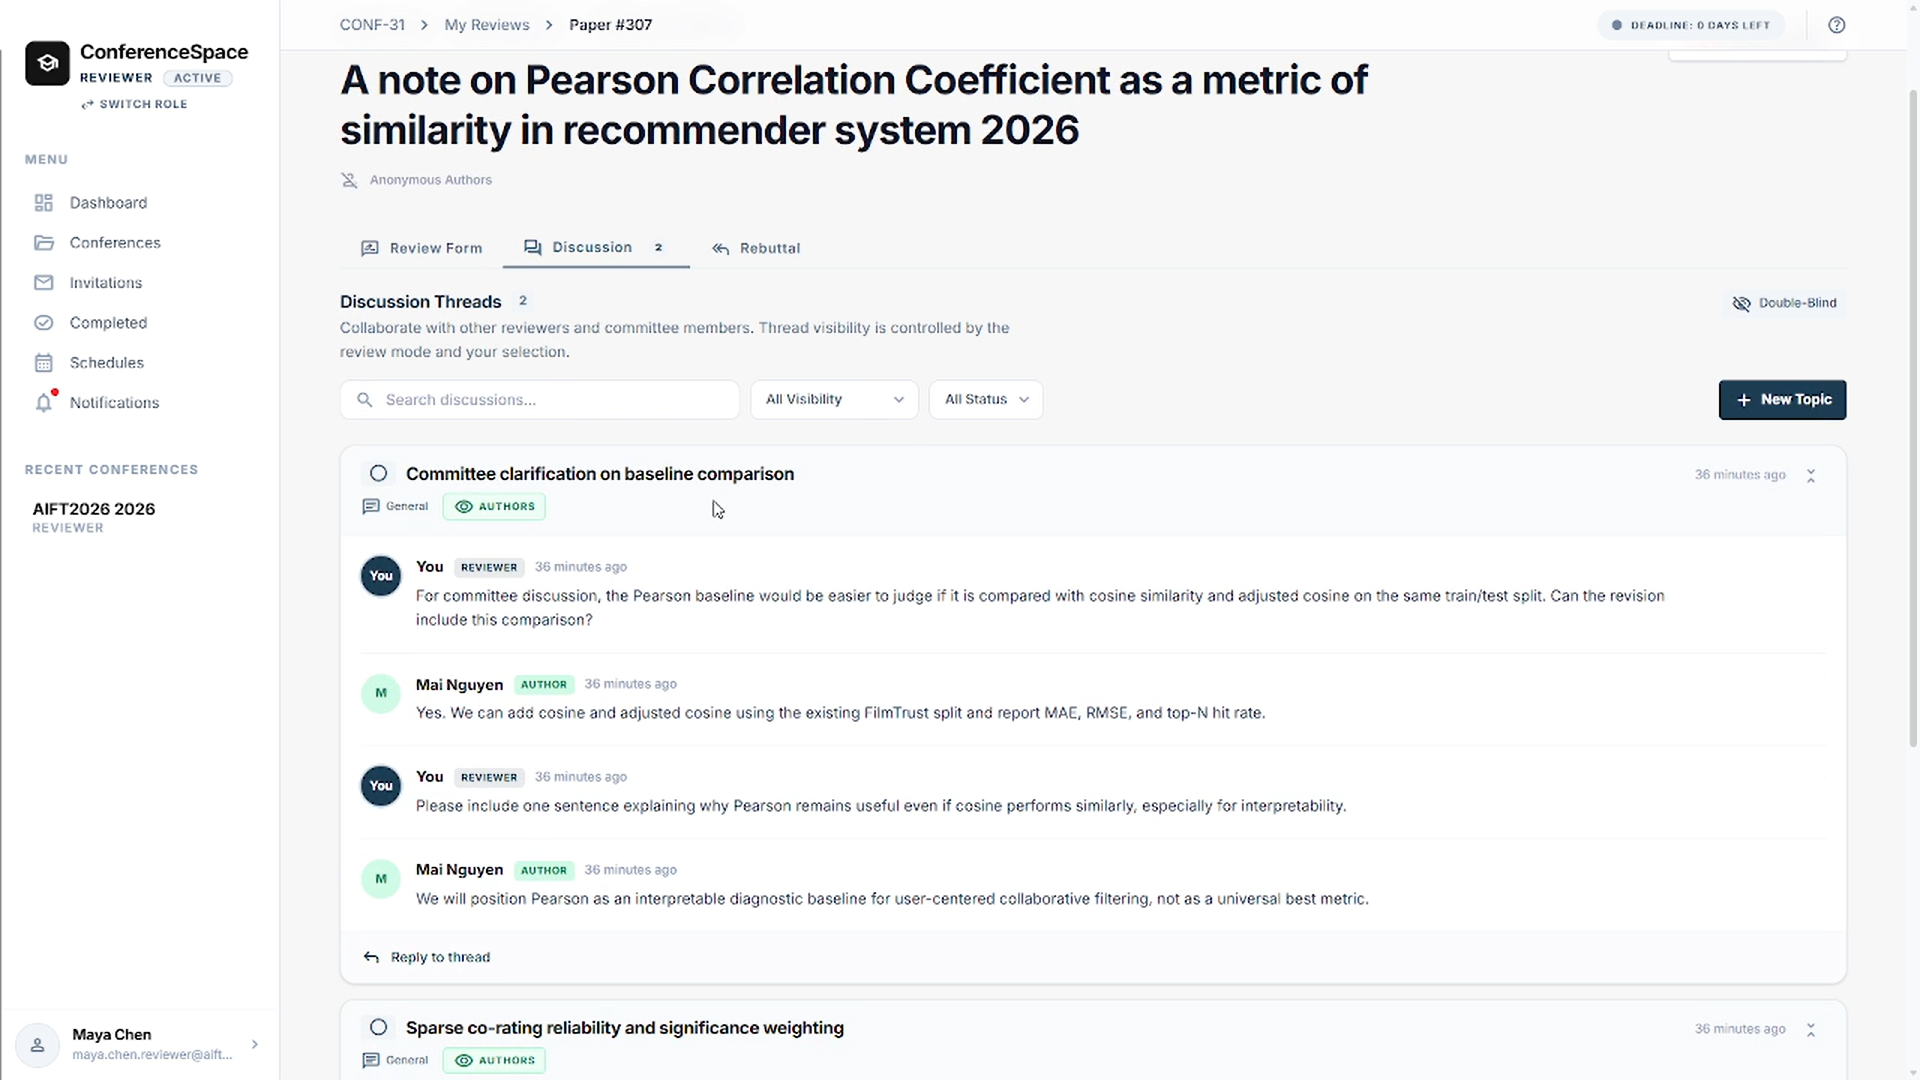
\includegraphics[width=0.95\textwidth]{images/chapter_3_uc08_discussion_chat.png}
  \caption{Giao diện hiển thị danh sách và trao đổi nội dung thảo luận}
  \label{fig:uc08-discussion-chat-cut}
\end{figure}

Hình~\ref{fig:uc08-discussion-chat-cut} thể hiện giao diện hiển thị danh sách chủ đề và nội dung trao đổi trong từng chủ đề.

\subsubsection{UC-09. Tổng hợp bằng chứng hỗ trợ Chủ tọa ra quyết định}

Backend tập hợp điểm số, bản phản biện, phản hồi của Tác giả, thay đổi sau phản hồi và nội dung thảo luận. Chair Decision Copilot tổ chức các nguồn này thành bản tổng hợp gồm điểm đồng thuận, bất đồng, vấn đề còn mở và bằng chứng liên quan. Chủ tọa đối chiếu bản tổng hợp với dữ liệu gốc rồi tự ghi nhận quyết định cuối cùng. Khi bộ bằng chứng thay đổi, hệ thống đánh dấu kết quả cũ là không còn hiệu lực.

\begin{figure}[H]
  \centering
  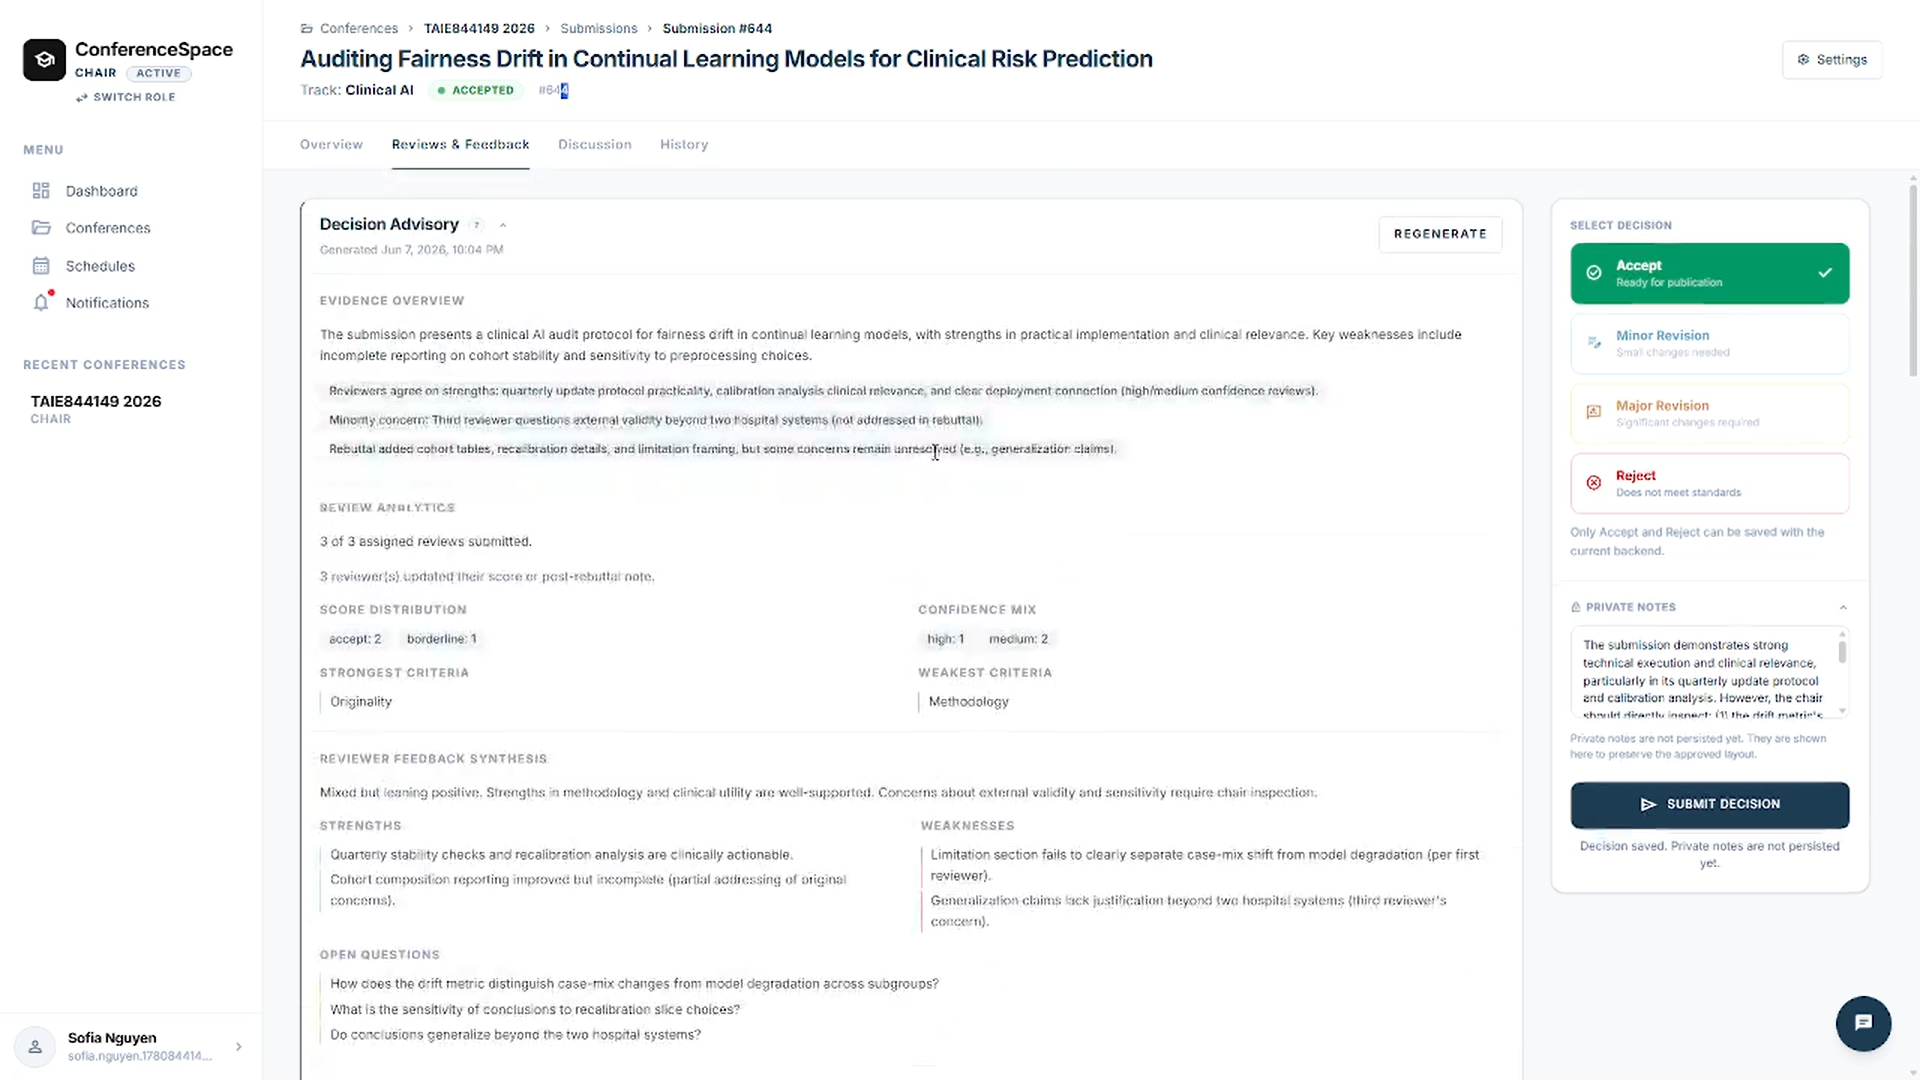
\includegraphics[width=0.95\textwidth]{images/chapter_3_uc09_decision_support.png}
  \caption{Giao diện tổng hợp bằng chứng và ghi nhận quyết định của Chủ tọa}
  \label{fig:uc09-decision-cut}
\end{figure}

Hình~\ref{fig:uc09-decision-cut} minh họa giao diện tổng hợp bằng chứng và ghi nhận quyết định của Chủ tọa.

Chair Decision Copilot không tạo khuyến nghị chấp nhận hoặc từ chối. Khi dịch vụ AI gặp lỗi, Chủ tọa vẫn có thể đọc trực tiếp các nguồn bằng chứng và tiếp tục quy trình nghiệp vụ.

\subsubsection{UC-10. Truy vấn trạng thái và hướng dẫn theo ngữ cảnh bằng Chatbot Agent}

Chatbot Agent nhận câu hỏi, lịch sử hội thoại và ngữ cảnh trang hiện tại. Nếu câu hỏi cần dữ liệu nghiệp vụ, Chatbot Agent gọi công cụ truy vấn để gửi yêu cầu có cấu trúc đến backend; backend kiểm tra mã xác thực, tài nguyên, trường dữ liệu, bộ lọc và quyền của người dùng trước khi trả phần dữ liệu tối thiểu được phép. Chatbot Agent dùng kết quả này để tạo câu trả lời phù hợp với vai trò và không truy cập trực tiếp cơ sở dữ liệu.

Backend từ chối yêu cầu vượt quá quyền truy cập; Chatbot Agent thông báo rõ khi câu hỏi nằm ngoài phạm vi chức năng được hỗ trợ. Khi công cụ gặp lỗi, hệ thống trả trạng thái lỗi thay vì tạo dữ liệu không có căn cứ. Các kịch bản hội thoại ở Chương 4 kiểm tra ranh giới này trong phạm vi tài nguyên và vai trò đã chọn.

\begin{figure}[H]
  \centering
  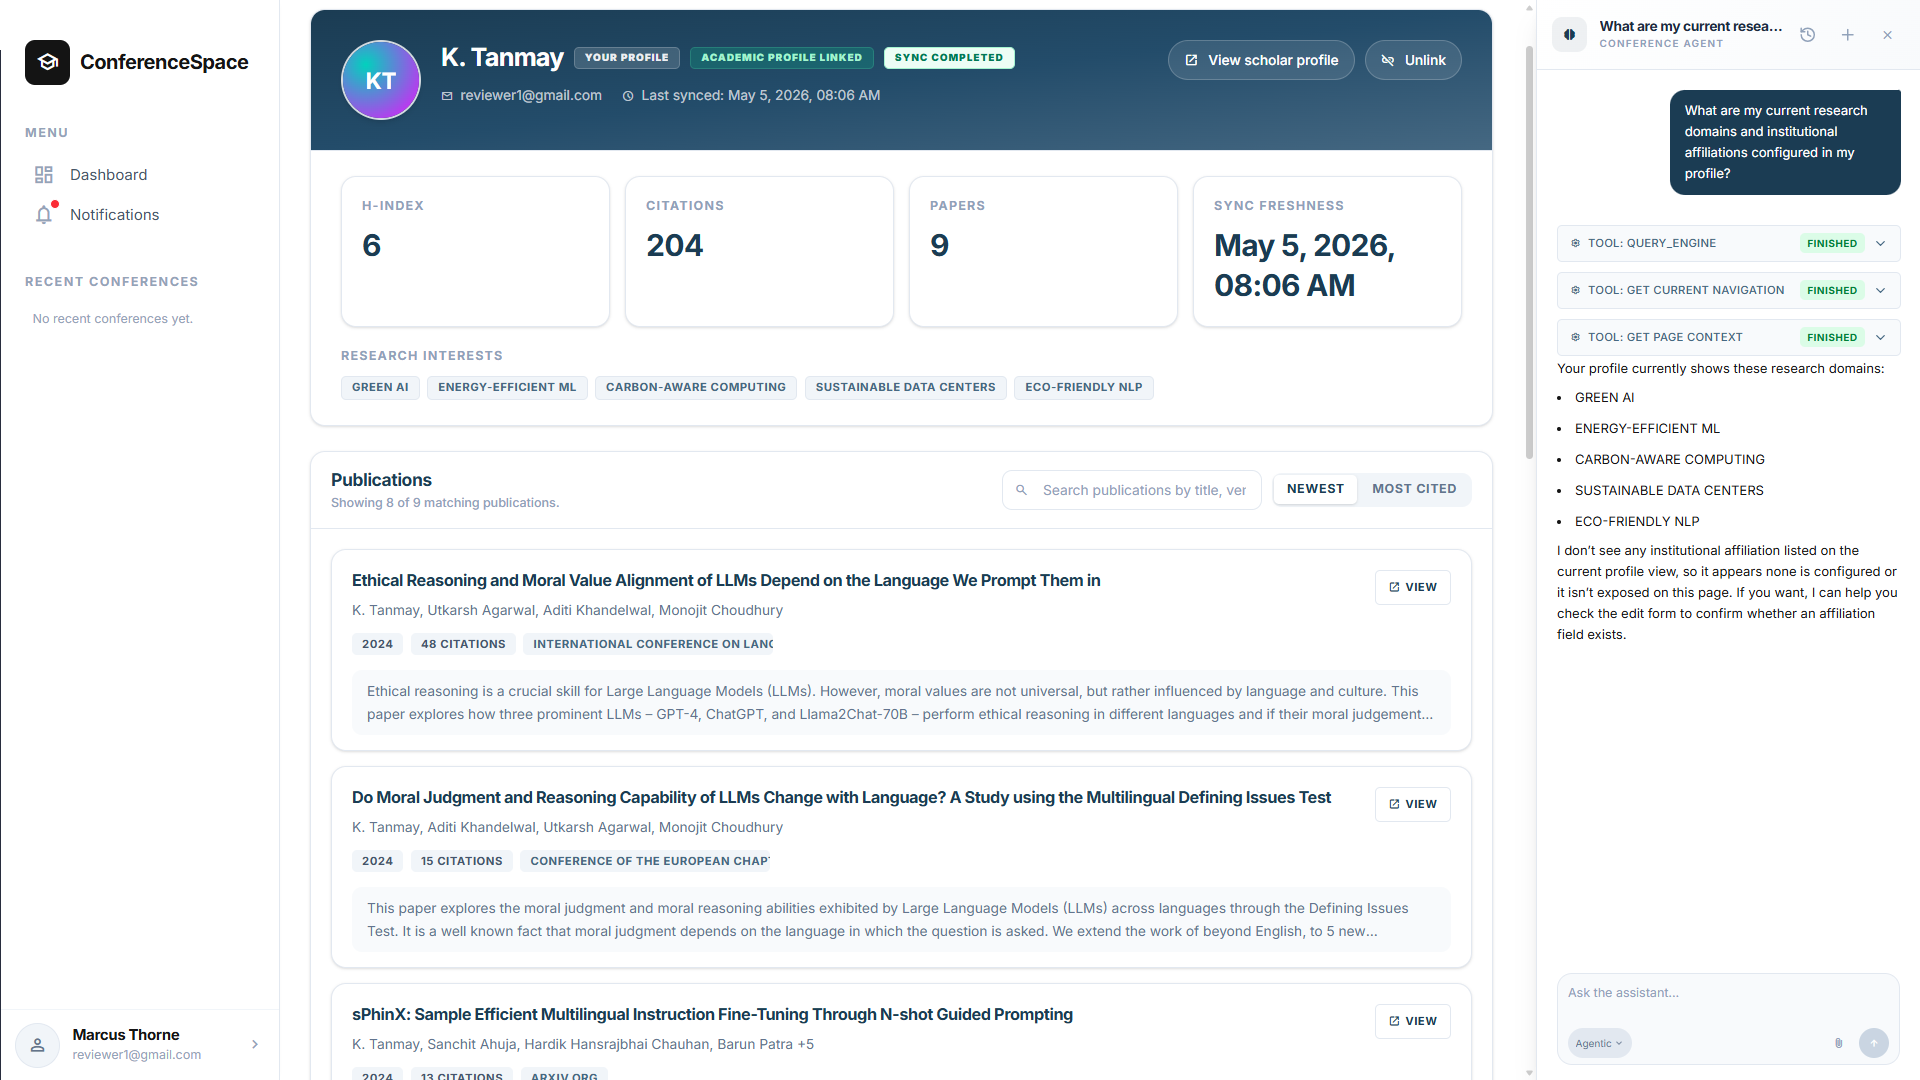
\includegraphics[width=0.95\textwidth]{images/chapter_3_uc10_chatbot_interface.png}
  \caption{Giao diện hội thoại và hỗ trợ tra cứu thông tin của Chatbot Agent}
  \label{fig:uc10-chatbot-cut}
\end{figure}

Hình~\ref{fig:uc10-chatbot-cut} minh họa giao diện hội thoại của Chatbot Agent trong luồng này.

\section{Thiết kế kỹ thuật}

\subsection{Kiến trúc tổng thể}
\label{subsec:ch3-architecture-cut}

ConferenceSpace gồm giao diện web Next.js, backend Go/Gin, dịch vụ AI FastAPI, PostgreSQL, Redis, Neo4j và cổng Caddy. Backend nghiệp vụ là một ứng dụng nguyên khối có kiến trúc phân lớp; nhóm không chia nhỏ nghiệp vụ thành các vi dịch vụ khi chưa có nhu cầu vận hành tương ứng. Dịch vụ AI và các kho dữ liệu được tách tại ranh giới triển khai vì có vòng đời, tải xử lý và yêu cầu truy cập khác với backend.

\begin{figure}[H]
  \centering
  \begin{adjustbox}{max width=\textwidth}
    \begin{tikzpicture}[node distance=12mm and 18mm, >=Latex]
      \node[prismNode] (browser) at (0,0) {Trình duyệt};
      \node[prismNode] (caddy) at (0,-2.2) {Caddy};
      \node[prismNode] (web) at (0,-4.4) {Next.js};
      \node[prismNode] (backend) at (0,-6.6) {Backend Go/Gin};
      \node[prismNode] (postgres) at (-6.4,-9.2) {PostgreSQL};
      \node[prismNode] (neo4j) at (-2.1,-9.2) {Neo4j};
      \node[prismNode] (ai) at (2.1,-9.2) {Dịch vụ AI};
      \node[prismNode] (external) at (6.4,-9.2) {Nguồn dữ liệu học thuật bên ngoài};
      \node[prismNode] (redis) at (0,-11.8) {Redis};
      \node[prismNode] (model) at (4.3,-11.8) {Nhà cung cấp mô hình};
      \draw[prismArrow] (browser) -- (caddy);
      \draw[prismArrow] (caddy) -- (web);
      \draw[prismArrow] (web) -- (backend);
      \draw[prismArrow] (web) -- node[prismEdgeLabel] {API hội thoại} (ai);
      \draw[prismArrow] (backend) -- (postgres);
      \draw[prismArrow] (backend) -- (neo4j);
      \draw[prismArrow] (backend) -- (ai);
      \draw[prismDashedArrow, bend left=24] (ai) to node[prismEdgeLabel] {endpoint truy vấn của backend} (backend);
      \draw[prismArrow] (backend) -- (external);
      \draw[prismArrow] (ai) -- (redis);
      \draw[prismArrow] (ai) -- (model);
      \draw[prismDashedArrow] (ai) -- node[prismEdgeLabel] {kết quả cần truy vết} (postgres);
    \end{tikzpicture}
  \end{adjustbox}
  \caption{Kiến trúc dịch vụ và ranh giới dữ liệu của ConferenceSpace}
  \label{fig:ch3-architecture-cut}
\end{figure}

Backend là ranh giới nghiệp vụ chính đối với dữ liệu và cập nhật trạng thái. Giao diện không truy cập trực tiếp cơ sở dữ liệu hoặc nhà cung cấp mô hình; tuy nhiên, Next.js có luồng giao tiếp trực tiếp với dịch vụ AI cho hội thoại. Khi Chatbot Agent cần dữ liệu nghiệp vụ, dịch vụ AI gọi endpoint truy vấn của backend bằng mã xác thực của người dùng và mã xác thực liên dịch vụ; backend tiếp tục kiểm tra danh mục tài nguyên và phân quyền theo vai trò trong hội nghị (RBAC). Sơ đồ vì vậy tách luồng hội thoại Next.js--AI khỏi luồng truy vấn dữ liệu AI--backend.

\subsection{Thiết kế giao diện web và trải nghiệm theo vai trò}
\label{subsec:ch3-web-cut}

Giao diện được tổ chức theo không gian làm việc của từng vai trò. Không gian Tác giả kết nối hoạt động khám phá hội nghị, nộp và quản lý bài; không gian Phản biện viên kết nối lời mời, bài được phân công, trình soạn phản biện và thảo luận; không gian Chủ tọa kết nối cấu hình, phân công, giám sát tiến độ và ra quyết định. Chatbot Agent và thông báo xuất hiện trong cả ba không gian nhưng dùng cùng ngữ cảnh xác thực và quyền trên tài nguyên.

Giao diện sử dụng Next.js App Router, React, TypeScript, Radix UI và Tailwind CSS \cite{ch3ref1,ch3ref3,ch3ref4,ch3ref5}. Các luồng dài được chia thành từng bước; trạng thái quan trọng được thể hiện bằng nhãn và bảng; thao tác gửi bài, gửi phản biện và lưu quyết định yêu cầu người dùng xác nhận. Đầu ra AI được trình bày dưới dạng bản nháp, cảnh báo hoặc bản tổng hợp cần kiểm tra, thay vì kết luận chính thức.

\subsection{Thiết kế backend, API và phân quyền}
\label{subsec:ch3-backend-cut}

Backend áp dụng kiến trúc phân lớp. Tầng điều khiển tiếp nhận yêu cầu HTTP; tầng dịch vụ thực thi nghiệp vụ; tầng lưu trữ làm việc với PostgreSQL; tầng tích hợp (client) kết nối dịch vụ AI, Neo4j, nguồn dữ liệu học thuật và thư điện tử. Nghiệp vụ phân công được tách thành miền riêng để logic tính điểm, đối sánh và phát hiện xung đột lợi ích có thể được kiểm thử độc lập.

\begin{figure}[H]
  \centering
  \begin{adjustbox}{max width=0.9\textwidth}
    \begin{tikzpicture}[node distance=12mm and 18mm, >=Latex]
      \node[prismNode] (router) at (0,0) {Bộ định tuyến Gin};
      \node[prismNode] (middleware) at (0,-2.2) {Middleware xác thực và ghi nhật ký};
      \node[prismNode] (controller) at (0,-4.4) {Tầng điều khiển};
      \node[prismNode] (service) at (0,-6.6) {Tầng dịch vụ};
      \node[prismNode] (storage) at (-4.2,-9.0) {Tầng lưu trữ};
      \node[prismNode] (assignment) at (0,-9.0) {Miền phân công};
      \node[prismNode] (clients) at (4.2,-9.0) {Tầng tích hợp};
      \node[prismNode] (db) at (-4.2,-11.4) {PostgreSQL};
      \node[prismNode] (coi) at (0,-11.4) {Đối sánh và xung đột lợi ích};
      \node[prismNode] (services) at (4.2,-11.4) {AI, Neo4j, email};
      \draw[prismArrow] (router) -- (middleware);
      \draw[prismArrow] (middleware) -- (controller);
      \draw[prismArrow] (controller) -- (service);
      \draw[prismArrow] (service) -- (storage);
      \draw[prismArrow] (service) -- (assignment);
      \draw[prismArrow] (service) -- (clients);
      \draw[prismArrow] (storage) -- (db);
      \draw[prismArrow] (assignment) -- (coi);
      \draw[prismArrow] (clients) -- (services);
    \end{tikzpicture}
  \end{adjustbox}
  \caption{Kiến trúc phân tầng của backend}
  \label{fig:ch3-backend-cut}
\end{figure}

Hệ thống phân quyền theo vai trò trong từng hội nghị thay vì dùng quyền toàn cục. Một người có thể là Tác giả ở hội nghị này, Phản biện viên ở hội nghị khác và Chủ tọa ở hội nghị thứ ba; do đó, backend kiểm tra cả danh tính người dùng và quan hệ của họ với tài nguyên cụ thể. Bảng~\ref{tab:ch3-discussion-permission-cut} minh họa cách nguyên tắc này được áp dụng cho chức năng thảo luận.

\begin{table}[H]
  \centering
  \caption{Quyền hiện hành trong chức năng thảo luận theo bài nộp}
  \label{tab:ch3-discussion-permission-cut}
  \setlength{\tabcolsep}{2pt}
  \renewcommand{\arraystretch}{1.15}
  \begin{tabularx}{\textwidth}{|P{0.22\textwidth}|Y|Y|Y|}
    \hline
    \TableHeader{Vai trò} & \TableHeader{Tạo chuỗi} & \TableHeader{Xem chuỗi} & \TableHeader{Gửi tin nhắn} \\ \hline
    Phản biện viên được phân công & Có & Các chuỗi do mình tạo trong bài nộp & Có, trong chuỗi do mình tạo \\ \hline
    Tác giả của bài nộp & Không & Các chuỗi gắn với bài của mình & Có, trong chuỗi liên quan \\ \hline
    Chủ tọa/Đồng chủ tọa & Không & Toàn bộ chuỗi và tin nhắn của bài & Không \\ \hline
  \end{tabularx}
\end{table}

Ngoài JWT dành cho người dùng cuối, hệ thống dùng mã xác thực riêng cho tác vụ quản trị nội bộ và giao tiếp giữa dịch vụ AI với endpoint truy vấn của backend. Mã xác thực dịch vụ không thay thế kiểm tra quyền: backend vẫn giới hạn tài nguyên, trường dữ liệu và thao tác theo người dùng hiện tại.

\subsection{Thiết kế cơ sở dữ liệu và lưu trữ dữ liệu}

ConferenceSpace phân chia dữ liệu theo yêu cầu giao dịch và kiểu truy vấn. PostgreSQL lưu dữ liệu nghiệp vụ, phiên và tin nhắn hội thoại cùng kết quả cần truy vết; Neo4j lưu quan hệ đồng tác giả để truy vấn nhiều bậc; Redis lưu kết quả công cụ đang chờ và bộ đếm giới hạn tần suất có thời hạn ngắn. Bảng~\ref{tab:ch3-db-groups-cut} tóm tắt bốn nhóm dữ liệu chính và vai trò của chúng.

\begingroup
\setlength{\tabcolsep}{2pt}
\begin{longtable}{|P{0.27\textwidth}|P{0.30\textwidth}|P{0.35\textwidth}|}
  \caption{Nhóm dữ liệu chính trong thiết kế cơ sở dữ liệu}\label{tab:ch3-db-groups-cut}\\
  \hline
  \TableHeader{Nhóm dữ liệu} & \TableHeader{Thực thể tiêu biểu} & \TableHeader{Vai trò trong thiết kế} \\ \hline
  \endfirsthead
  \hline
  \TableHeader{Nhóm dữ liệu} & \TableHeader{Thực thể tiêu biểu} & \TableHeader{Vai trò trong thiết kế} \\ \hline
  \endhead
  Nghiệp vụ hội nghị & \textit{conferences}, \CodeBreak{conference\_submissions}, \CodeBreak{paper\_assignments}, \CodeBreak{rebuttal\_points} & Bảo toàn vòng đời nộp bài--phản biện--phản hồi và các ràng buộc giao dịch \\ \hline
  Phân quyền và phối hợp & \textit{users}, \CodeBreak{conference\_user\_roles}, \CodeBreak{discussion\_threads}, \textit{notifications} & Giới hạn thao tác theo vai trò, tài nguyên và chuyển thông báo đến đúng người \\ \hline
  Học thuật và xung đột lợi ích & \CodeBreak{scholar\_profiles}, \CodeBreak{scholar\_papers}, \CodeBreak{coi\_relationships}, đồ thị Neo4j & Phát hiện quan hệ có nguy cơ gây xung đột và lưu bằng chứng để Chủ tọa kiểm tra \\ \hline
  Kết quả AI và kiểm toán & \textit{ai.*\_runs}, \textit{ai.*\_artifacts}, \textit{ai.*\_stage\_records}, \textit{ai\_tool\_audit} & Theo dõi đầu vào, đầu ra, trạng thái và lỗi của từng luồng AI \\ \hline
\end{longtable}
\endgroup

\begin{figure}[H]
  \centering
  \begin{adjustbox}{max width=\textwidth}
    \begin{tikzpicture}[
        entity/.style={draw=black!65, rounded corners=2pt, align=center, font=\scriptsize\ttfamily, text width=3.5cm, minimum height=9mm, fill=green!6},
        fk/.style={-{Latex[length=1.8mm]}, thick, draw=black!75},
        logical/.style={-{Latex[length=1.8mm]}, thick, dashed, draw=blue!65!black},
        relLabel/.style={font=\scriptsize, align=center, fill=white, inner sep=1pt},
        legend/.style={draw=black!45, rounded corners=2pt, align=left, font=\scriptsize, fill=white, inner sep=3pt}
      ]
      \node[entity] (users) at (-7.2,0) {users};
      \node[entity] (conferences) at (-2.4,0) {conferences};
      \node[entity] (roles) at (2.4,0) {conference\_user\_roles};
      \node[entity] (sessions) at (7.2,0) {ai\_sessions / ai\_messages};

      \node[entity] (scholar) at (-7.2,-2.4) {scholar\_profiles};
      \node[entity] (submissions) at (-2.4,-2.4) {conference\_submissions};
      \node[entity] (reviewers) at (2.4,-2.4) {conference\_reviewers};
      \node[entity] (coi) at (7.2,-2.4) {coi\_relationships};

      \node[entity] (rebuttal) at (-7.2,-4.8) {rebuttal\_points};
      \node[entity] (assignments) at (-2.4,-4.8) {paper\_assignments};
      \node[entity] (audit) at (2.4,-4.8) {review\_audit\_events};
      \node[entity] (threads) at (7.2,-4.8) {discussion\_threads};
      \node[entity] (messages) at (7.2,-7.2) {discussion\_messages};

      \draw[fk] (users) -- node[relLabel] {1:0..1} (scholar);
      \draw[fk] (submissions) -- node[relLabel] {1:N} (assignments);
      \draw[fk] (reviewers) -- node[relLabel, pos=0.58] {1:N} (assignments);
      \draw[fk] (assignments) -- node[relLabel] {1:N} (audit);
      \draw[fk] (submissions.east) -- ++(0.8,0) |- node[relLabel, pos=0.73] {1:N} (threads.west);
      \draw[fk] (threads) -- node[relLabel] {1:N} (messages);

      \draw[logical] (users) -- node[relLabel] {định danh} (roles);
      \draw[logical] (conferences) -- node[relLabel] {phạm vi} (roles);
      \draw[logical] (conferences) -- node[relLabel] {phạm vi} (submissions);
      \draw[logical] (users.south east) to[bend left=14] node[relLabel, pos=0.55] {vai trò} (reviewers.north west);
      \draw[logical] (conferences.south east) -- node[relLabel] {phạm vi} (reviewers.north west);
      \draw[logical] (submissions) -- node[relLabel] {định danh} (rebuttal);
      \draw[logical] (submissions.east) to[bend left=12] node[relLabel, pos=0.72] {định danh} (coi.west);
      \draw[logical] (reviewers) -- node[relLabel] {định danh} (coi);
      \draw[logical] (users) -- node[relLabel] {định danh} (sessions);

      \node[legend, anchor=north west] at (-7.2,-7.0) {
        \tikz\draw[fk] (0,0) -- (0.9,0);\; khóa ngoại được PostgreSQL cưỡng chế\\[2pt]
        \tikz\draw[logical] (0,0) -- (0.9,0);\; quan hệ logic qua định danh hoặc tầng ứng dụng
      };
    \end{tikzpicture}
  \end{adjustbox}
  \caption{Các thực thể triển khai và quan hệ chính trong PostgreSQL}
  \label{fig:ch3-data-cut}
\end{figure}

Hình~\ref{fig:ch3-data-cut} giữ nguyên định danh kỹ thuật và phân biệt khóa ngoại vật lý với quan hệ được nối ở tầng ứng dụng. \CodeBreak{paper\_assignments.reviewer\_id} tham chiếu \CodeBreak{conference\_reviewers.id}; từ đó hệ thống mới xác định người dùng giữ vai trò Phản biện viên trong một hội nghị. Nét đứt không biểu thị ràng buộc khóa ngoại trong PostgreSQL. \CodeBreak{coi\_relationships} lưu bằng chứng do quy trình refresh hoặc rebuild tạo ra, còn bản đồ xung đột dùng để loại cặp xung đột được xây dựng riêng cho từng lượt đối sánh.

Reviewer Initial Analysis và Chair Decision Copilot dùng mã nhận diện đầu vào (fingerprint) để phát hiện kết quả không còn hiệu lực (\textit{stale}) khi dữ liệu nguồn thay đổi. Reviewer Initial Analysis tính mã này từ trạng thái bài nộp; Chair Decision Copilot tính mã cho bộ bằng chứng và từng thành phần, đồng thời lưu lý do hết hiệu lực. Submission Gating ghi mã nhận diện đầu vào cùng mã chính sách cho mỗi lần chạy, còn Review Quality Auditor lưu yêu cầu, phản hồi, trạng thái lần chạy và mã nhận diện của điều kiện phát hiện.

Submission Autofill không lưu kết quả theo cơ chế hết hiệu lực mà trả dữ liệu để Tác giả áp dụng vào biểu mẫu có thể chỉnh sửa. Chatbot Agent lưu phiên và lịch sử hội thoại để phục vụ truy vết.

\subsection{Luồng xử lý hệ thống}

\subsubsection{Luồng nộp bài có AI hỗ trợ}

Trong luồng nộp bài, giao diện chuyển tệp và ngữ cảnh hội nghị đến backend; backend gọi Submission Autofill để tạo bản nháp, sau đó lưu các chỉnh sửa do Tác giả xác nhận. Trước khi gửi chính thức, backend gửi bản nháp hiện hành đến Submission Gating để kiểm tra. AI chỉ tạo dữ liệu hỗ trợ và cảnh báo; backend kiểm soát việc ghi dữ liệu chính thức, còn Tác giả quyết định gửi bài. Tác giả có thể tiếp tục nhập và lưu bản nháp khi chức năng AI không khả dụng; thao tác gửi bài vẫn cần một kết quả Submission Gating hợp lệ.

\subsubsection{Luồng Chatbot Agent truy vấn dữ liệu hệ thống}

Chatbot Agent chỉ gọi endpoint truy vấn mà backend đã định nghĩa và cho phép sử dụng. Mỗi yêu cầu gồm ngữ cảnh người dùng, tài nguyên, trường dữ liệu và điều kiện truy vấn; backend xác thực người dùng và dịch vụ, kiểm tra danh mục tài nguyên rồi mới thực thi. Cách tổ chức này giữ việc kiểm soát quyền tại backend và ngăn Chatbot Agent sử dụng quyền truy cập cơ sở dữ liệu trực tiếp.

\section{Cơ chế nghiệp vụ và thuật toán xác định}

\subsection{Vai trò của các cơ chế xác định}

Các tác vụ có quy tắc rõ ràng được tách khỏi lớp AI để người dùng có thể kiểm tra điều kiện và nguyên nhân của kết quả. Nhóm này gồm đối sánh Phản biện viên, phát hiện xung đột lợi ích, kiểm soát trạng thái và hạn chót nộp bài, phân quyền, định tuyến thông báo và kiểm tra cấu trúc dữ liệu. Kết quả chỉ ổn định khi hệ thống đã định nghĩa đầy đủ quy tắc, bao gồm cách phân xử các trường hợp bằng điểm.

\subsection{Đối sánh phản biện viên}
\label{subsec:ch3-matching-cut}

Hệ thống tạo đề xuất phân công từ miền chuyên môn của bài nộp và Phản biện viên, cấu hình hội nghị cùng kết quả kiểm tra xung đột lợi ích. Matcher hiện chỉ nhận đầu vào là định danh Phản biện viên, không kèm dữ liệu tải hiện có; do đó bộ đếm tải được khởi tạo bằng $0$ và chỉ phản ánh số phân công phát sinh trong lượt chạy, không bao gồm các phân công đã tồn tại trước đó. Với tập miền chuyên môn của bài nộp $S$ và của Phản biện viên $R$, điểm phù hợp được tính bằng hệ số Jaccard:

\[
  J(S,R)=\frac{|S\cap R|}{|S\cup R|}.
\]

Nếu cả hai tập rỗng, hệ thống gán điểm $0$ vì không có bằng chứng về mức độ phù hợp. Nhóm chọn Jaccard vì điểm số có thể giải thích trực tiếp từ số miền chuyên môn chung và không cần mô hình học máy hoặc dữ liệu huấn luyện. Chiến lược tham lam lần lượt chọn các cặp có điểm cao, nhờ đó đơn giản hóa việc triển khai và kiểm tra so với việc giải bài toán tối ưu toàn cục. Đổi lại, Jaccard xem các miền chuyên môn như tập hợp không trọng số; chiến lược tham lam có thể bỏ lỡ phương án có tổng mức phù hợp cao hơn cho toàn bộ hội nghị và phụ thuộc vào thứ tự khi nhiều cặp bằng điểm.

Hình~\ref{fig:ch3-matching-flow-cut} biểu diễn hai lượt của thuật toán và ràng buộc được giữ hoặc nới ở mỗi lượt.

\begin{figure}[H]
  \centering
  \begin{adjustbox}{max width=0.90\textwidth, max height=0.70\textheight, keepaspectratio}
    \begin{tikzpicture}[scale=0.84, every node/.style={transform shape},
        matchStep/.style={draw=black!65, rounded corners=2pt, align=center, font=\footnotesize, text width=4.2cm, minimum height=11mm, fill=blue!7},
        pass/.style={draw=black!65, rounded corners=2pt, align=left, font=\footnotesize, text width=5.5cm, minimum height=20mm, fill=green!7},
        decision/.style={draw=black!65, diamond, aspect=2.2, align=center, font=\scriptsize, text width=2.8cm, fill=orange!9},
        end/.style={draw=black!65, rounded corners=2pt, align=center, font=\footnotesize, text width=4.6cm, minimum height=11mm, fill=gray!9},
        >=Latex
      ]
      \node[matchStep] (matrix) at (0,0) {Tạo ma trận điểm Jaccard cho các cặp bài nộp--Phản biện viên};
      \node[matchStep] (filter) at (0,-2.2) {Loại các cặp có xung đột lợi ích};
      \node[matchStep] (sort) at (0,-4.4) {Sắp xếp điểm giảm dần\\chưa có tiêu chí phân xử khi bằng điểm};
      \node[pass] (pass1) at (0,-7.3) {\textbf{Lượt 1}\newline Giữ ngưỡng điểm, số người cần cho mỗi bài, giới hạn tải phát sinh trong lượt chạy và xung đột lợi ích};
      \node[decision] (unassigned) at (0,-10.7) {Bài nào vẫn có 0 Phản biện viên?};
      \node[pass] (pass2) at (5.8,-13.8) {\textbf{Lượt 2}\newline Bỏ ngưỡng điểm và giới hạn tải; vẫn giữ xung đột lợi ích; chỉ bổ sung một Phản biện viên};
      \node[end] (result) at (0,-17.0) {Trả đề xuất, điểm số và danh sách bài còn thiếu người};
      \node[end, fill=orange!7] (confirm) at (0,-19.4) {Chủ tọa xem, điều chỉnh và xác nhận};
      \draw[prismArrow] (matrix) -- (filter);
      \draw[prismArrow] (filter) -- (sort);
      \draw[prismArrow] (sort) -- (pass1);
      \draw[prismArrow] (pass1) -- (unassigned);
      \draw[prismArrow] (unassigned) -- node[prismEdgeLabel] {Có} (pass2);
      \draw[prismArrow] (unassigned) -- node[prismEdgeLabel] {Không} (result);
      \draw[prismArrow] (pass2) -- (result);
      \draw[prismArrow] (result) -- (confirm);
    \end{tikzpicture}
  \end{adjustbox}
  \caption{Hai lượt của thuật toán đối sánh GreedyMatcher}
  \label{fig:ch3-matching-flow-cut}
\end{figure}

Lượt dự phòng có thể chọn cặp có điểm bằng $0$ hoặc làm Phản biện viên vượt giới hạn tải trong lượt chạy; thủ tục cũng không bảo đảm mọi bài có đủ số người yêu cầu. Vì vậy, đầu ra gồm điểm, lý do, số phân công được tạo cho từng Phản biện viên và danh sách bài còn thiếu người để Chủ tọa kiểm tra trước khi xác nhận. Do chưa có tiêu chí phân xử thứ cấp khi bằng điểm và chưa tính đến tải lịch sử của Phản biện viên, báo cáo không dùng thuật toán này làm bằng chứng cho tính tái tạo hoàn toàn hoặc cân bằng tổng tải hiện có.

\begin{table}[H]
  \centering
  \caption{Tình huống ngoại lệ trong đối sánh Phản biện viên}
  \label{tab:ch3-matching-exceptions-cut}
  \setlength{\tabcolsep}{3pt}
  \renewcommand{\arraystretch}{1.15}
  \begin{tabularx}{\textwidth}{|Y|Y|}
    \hline
    \TableHeader{Tình huống} & \TableHeader{Cách xử lý} \\ \hline
    Bài nộp không có đủ Phản biện viên không có xung đột lợi ích & Đánh dấu thiếu để Chủ tọa mời thêm hoặc phân công thủ công \\ \hline
    Hồ sơ thiếu miền chuyên môn & Giữ ứng viên với điểm thấp nếu không có xung đột lợi ích, nhưng không ưu tiên \\ \hline
    Không cấu hình kết nối Neo4j & Áp dụng các lớp kiểm tra còn lại và ghi trạng thái \CodeBreak{skipped\_neo4j\_unavailable}; độ bao phủ quan hệ bị giảm \\ \hline
    Tất cả ứng viên có điểm phù hợp đều có xung đột lợi ích & Thuật toán tự động không gán và giữ bài nộp trong danh sách thiếu Phản biện viên \\ \hline
  \end{tabularx}
\end{table}

Thuật toán tự động tạo danh sách đề xuất và cung cấp căn cứ để Chủ tọa kiểm tra trước khi xác nhận. Bộ đếm tải chỉ bao gồm các phân công phát sinh trong lượt chạy hiện tại, còn trường hợp bằng điểm chưa có tiêu chí phân xử thứ cấp; đây là hai ranh giới trực tiếp của phương án hiện hành.

\subsection{Phát hiện xung đột lợi ích}
\label{subsec:ch3-coi-cut}

Hệ thống kiểm tra xung đột lợi ích theo ba nguồn bổ sung cho nhau: quan hệ tác giả của bài, khai báo thủ công và quan hệ đồng tác giả nhiều bậc trong Neo4j. \CodeBreak{coi\_relationships} lưu bằng chứng đã phát hiện để Chủ tọa kiểm tra, còn bản đồ xung đột được tạo cho lượt đối sánh là dữ liệu trực tiếp quyết định cặp nào bị loại khỏi thuật toán tự động. Hai cấu trúc phục vụ hai mục đích khác nhau và không được xem là thay thế cho nhau.

\begin{figure}[H]
  \centering
  \begin{adjustbox}{max width=\textwidth}
    \begin{tikzpicture}[
        source/.style={draw=black!65, rounded corners=2pt, align=center, font=\footnotesize, text width=3.5cm, minimum height=12mm, fill=blue!7},
        process/.style={draw=black!65, rounded corners=2pt, align=center, font=\footnotesize, text width=4.5cm, minimum height=13mm, fill=green!7},
        warning/.style={draw=black!65, rounded corners=2pt, align=center, font=\footnotesize, text width=4.7cm, minimum height=13mm, fill=orange!9},
        evidence/.style={draw=black!65, rounded corners=2pt, align=center, font=\footnotesize, text width=4.7cm, minimum height=13mm, fill=gray!9},
        lane/.style={draw=black!35, rounded corners=3pt, dashed, inner sep=5pt},
        laneTitle/.style={font=\scriptsize\bfseries, anchor=south west},
        >=Latex
      ]
      \node[source] (author) at (-5.2,0) {Tự phản biện và quan hệ đồng tác giả trực tiếp};
      \node[source] (declared) at (0,0) {Xung đột do Tác giả khai báo};
      \node[source] (graph) at (5.2,0) {Quan hệ đồng tác giả nhiều bậc qua Neo4j};

      \node[process] (map) at (-5.2,-3.1) {Tạo bản đồ xung đột cho lượt chạy};
      \node[process] (auto) at (-5.2,-5.8) {Đối sánh tự động loại cặp xung đột lợi ích trong cả hai lượt};

      \node[process] (rebuild) at (0,-3.1) {Tác vụ refresh/rebuild quan hệ xung đột lợi ích};
      \node[evidence] (stored) at (0,-5.8) {Ghi bằng chứng vào \CodeBreak{coi\_relationships}};

      \node[warning] (manualCheck) at (5.2,-3.1) {Đề xuất thủ công kiểm tra trực tiếp và đọc bộ nhớ đệm xung đột lợi ích nếu có};
      \node[warning] (manualResult) at (5.2,-5.8) {Trả \CodeBreak{COIWarning}; lưu trạng thái kiểm tra trong siêu dữ liệu của đề xuất};

      \draw[prismArrow] (author) -- (map);
      \draw[prismArrow] (declared) -- (map);
      \draw[prismArrow] (graph) -- (map);
      \draw[prismArrow] (map) -- (auto);

      \draw[prismArrow] (author) -- (rebuild);
      \draw[prismArrow] (declared) -- (rebuild);
      \draw[prismArrow] (graph) -- (rebuild);
      \draw[prismArrow] (rebuild) -- (stored);

      \draw[prismArrow] (author) -- (manualCheck);
      \draw[prismArrow] (declared) -- (manualCheck);
      \draw[prismDashedArrow] (stored) to[bend right=16] node[prismEdgeLabel] {bộ nhớ đệm nếu có} (manualCheck);
      \draw[prismArrow] (manualCheck) -- (manualResult);

      \node[laneTitle] at (-7.65,-1.7) {Cưỡng chế trong lượt đối sánh};
      \node[laneTitle] at (-2.45,-1.7) {Dữ liệu truy vết bền vững};
      \node[laneTitle] at (2.75,-1.7) {Cảnh báo cho đề xuất thủ công};
    \end{tikzpicture}
  \end{adjustbox}
  \caption{Ba luồng sử dụng kết quả phát hiện xung đột lợi ích}
  \label{fig:ch3-coi-flow-cut}
\end{figure}

Hình~\ref{fig:ch3-coi-flow-cut} tách ba mục đích sử dụng kết quả xung đột lợi ích. Bản đồ xung đột chỉ phục vụ lượt đối sánh tự động và loại cặp xung đột trước khi xếp hạng. \CodeBreak{coi\_relationships} được cập nhật qua tác vụ refresh hoặc rebuild riêng. Khi Chủ tọa thêm đề xuất thủ công, backend kiểm tra trực tiếp quan hệ tác giả, đồng tác giả và khai báo, đọc thêm bộ nhớ đệm xung đột lợi ích nếu có, trả \CodeBreak{COIWarning} và lưu trạng thái kiểm tra trong siêu dữ liệu của đề xuất; thao tác này không tự ghi quan hệ mới vào \CodeBreak{coi\_relationships}.

Thuật toán tự động không nới lỏng ràng buộc xung đột lợi ích trong lượt dự phòng. Khi thành phần phát hiện quan hệ chưa được cấu hình, hệ thống ghi \CodeBreak{skipped\_neo4j\_unavailable} và tiếp tục bằng các nguồn còn lại. Nếu truy vấn Neo4j thất bại, một số luồng chỉ ghi nhật ký lỗi rồi tiếp tục; khi đó, hệ thống không thể khẳng định rằng quan hệ đồng tác giả nhiều bậc đã được kiểm tra đầy đủ. Luồng thêm đề xuất thủ công hiện chỉ cảnh báo, chưa chặn ghi dữ liệu và chưa lưu bản ghi kiểm toán riêng cho quyết định tiếp tục.

\subsection{Các cơ chế nghiệp vụ hỗ trợ vận hành}
\label{subsec:ch3-operations-cut}

Các cơ chế hỗ trợ gồm máy trạng thái của hội nghị, kiểm soát hạn chót nộp bài, phân quyền theo vai trò trong hội nghị (RBAC), định tuyến thông báo và kiểm tra cấu trúc dữ liệu. Các cơ chế này kiểm tra và giới hạn thao tác theo vai trò, trạng thái và quy tắc đã được triển khai trước khi hệ thống ghi dữ liệu.

Cơ chế kiểm soát bản thảo hoàn chỉnh hiện chỉ kiểm tra bài ở trạng thái \textit{accepted} và tính hợp lệ của tệp; hệ thống chưa kiểm tra hạn chót nộp bản thảo hoàn chỉnh tại thời điểm thực thi. Giới hạn được nêu riêng vì đầu ra AI không thể bù cho một quy tắc nghiệp vụ chưa được áp dụng đầy đủ.

\section{Giải pháp AI}

\subsection{Vai trò của AI trong hệ thống}

AI được tích hợp vào sáu luồng hỗ trợ: Submission Autofill hỗ trợ nhập liệu; Submission Gating hỗ trợ kiểm tra bài nộp; Reviewer Initial Analysis hỗ trợ định hướng đọc; Review Quality Auditor hỗ trợ rà soát bản nháp; Chair Decision Copilot hỗ trợ tổng hợp bằng chứng; và Chatbot Agent hỗ trợ truy vấn dữ liệu. Bảng~\ref{tab:ch3-ai-overview-cut} đối chiếu đầu ra, điểm kiểm soát và ranh giới của từng luồng.

\begingroup
\setlength{\tabcolsep}{2pt}
\begin{longtable}{|P{0.17\textwidth}|P{0.26\textwidth}|P{0.23\textwidth}|P{0.26\textwidth}|}
  \caption{Dữ liệu và trạng thái của các luồng AI}\label{tab:ch3-ai-overview-cut}\\
  \hline
  \TableHeader{Luồng} & \TableHeader{Đầu vào} & \TableHeader{Đầu ra} & \TableHeader{Lỗi hoặc hiệu lực kết quả} \\ \hline
  \endfirsthead
  \hline
  \TableHeader{Luồng} & \TableHeader{Đầu vào} & \TableHeader{Đầu ra} & \TableHeader{Lỗi hoặc hiệu lực kết quả} \\ \hline
  \endhead
  Submission Autofill & Tệp và ngữ cảnh hội nghị & Siêu dữ liệu nháp, gợi ý chuyên đề & Cảnh báo khi thiếu dữ liệu; chưa lưu kết quả dưới dạng bản ghi có trạng thái \textit{stale} \\ \hline
  Submission Gating & Tệp và chính sách hội nghị & Trạng thái cùng phát hiện có bằng chứng & Ghi mã nhận diện đầu vào và mã chính sách; giữ kết quả kiểm tra theo quy tắc nếu riêng bước AI lỗi \\ \hline
  Reviewer Initial Analysis & Bản thảo và phân công & Bản định hướng đọc & Dùng mã nhận diện đầu vào để chuyển kết quả sang \textit{stale} khi bản thảo thay đổi \\ \hline
  Review Quality Auditor & Bản nháp phản biện và điểm & Danh sách phát hiện & Lưu trạng thái lần chạy và mã nhận diện của điều kiện phát hiện; lỗi thực thi được báo riêng \\ \hline
  Chair Decision Copilot & Bộ bằng chứng & Bản tổng hợp đồng thuận, bất đồng và vấn đề còn mở & Dùng mã nhận diện của bộ bằng chứng để đánh dấu \textit{stale} và nêu lý do \\ \hline
  Chatbot Agent & Câu hỏi, vai trò và ngữ cảnh trang & Câu trả lời cùng kết quả công cụ & Lưu phiên, lịch sử; công khai trạng thái bị từ chối, lỗi hoặc hết thời gian \\ \hline
\end{longtable}
\endgroup

\begin{table}[H]
  \centering
  \caption{Quyền xác nhận và tác động nghiệp vụ của các luồng AI}
  \label{tab:ch3-ai-authority-cut}
  \setlength{\tabcolsep}{3pt}
  \renewcommand{\arraystretch}{1.15}
  \begin{tabularx}{\textwidth}{|P{0.20\textwidth}|Y|Y|}
    \hline
    \TableHeader{Luồng} & \TableHeader{Điểm xác nhận của con người} & \TableHeader{Ranh giới tác động nghiệp vụ} \\ \hline
    Submission Autofill & Tác giả sửa và xác nhận; giao diện lọc chuyên đề hợp lệ & Chỉ cập nhật biểu mẫu, không tự gửi bài \\ \hline
    Submission Gating & Tác giả sửa lỗi hoặc xem cảnh báo & Kiểm tra theo quy tắc có thể tạo \textit{block}; bước đánh giá nội dung bằng AI chỉ tạo \textit{warn} hoặc \textit{pass} \\ \hline
    Reviewer Initial Analysis & Phản biện viên đối chiếu bài gốc & Không cập nhật điểm hoặc nội dung phản biện \\ \hline
    Review Quality Auditor & Phản biện viên xem, sửa hoặc gửi; xác nhận nếu bước rà soát thất bại & Nhãn \textit{blocking} chỉ làm nổi bật phát hiện, không ngăn gửi \\ \hline
    Chair Decision Copilot & Chủ tọa đối chiếu dữ liệu nguồn & Không ghi quyết định chấp nhận hoặc từ chối \\ \hline
    Chatbot Agent & Backend kiểm soát dữ liệu; người dùng xem kết quả & Chỉ đọc dữ liệu được phép, không cập nhật trạng thái chính thức \\ \hline
  \end{tabularx}
\end{table}

\subsection{Các luồng xử lý có sử dụng AI}
\label{subsec:ch3-ai-workflows-cut}

\subsubsection{Submission Autofill}

Submission Autofill đọc bản thảo để tạo bản nháp gồm tiêu đề, tóm tắt, từ khóa, thông tin tác giả và gợi ý chuyên đề. Đầu vào còn gồm ngữ cảnh hội nghị và danh sách chuyên đề đang mở. Cấu trúc phản hồi chưa tự giới hạn giá trị gợi ý vào danh sách này; khi áp dụng kết quả, giao diện đối chiếu và chỉ nhận các chuyên đề còn hợp lệ trong cấu hình hiện hành. Nếu văn bản trích xuất quá ít hoặc thiếu thông tin, luồng trả cảnh báo thay vì suy đoán dữ liệu.

Giao diện giữ toàn bộ trường ở trạng thái có thể chỉnh sửa; backend chỉ lưu bài nộp chính thức sau khi Tác giả xác nhận. Chương 4 đo độ khớp của siêu dữ liệu và kiểm tra gợi ý có thuộc danh sách chuyên đề hợp lệ. Phạm vi đánh giá chưa bao gồm nhãn chuyên gia cho thứ hạng chuyên đề; mức thời gian tiết kiệm được ước tính dựa trên phản hồi tự báo cáo, không phải phép đo trực tiếp thời gian hoàn thành biểu mẫu.

\subsubsection{Submission Gating}

Submission Gating kết hợp kiểm tra theo quy tắc và đánh giá nội dung có AI hỗ trợ. Luồng chuẩn hóa yêu cầu, kiểm tra tính toàn vẹn của tệp, trích xuất tài liệu, xác định dữ kiện, áp dụng chính sách hội nghị và tổng hợp phát hiện thành bốn trạng thái: \textit{pass}, \textit{warn}, \textit{block} hoặc \textit{error}.

\begin{figure}[H]
  \centering
  \begin{adjustbox}{max width=\textwidth}
    \begin{tikzpicture}[
        stage/.style={draw=black!65, rounded corners=2pt, align=center, font=\footnotesize, text width=4.2cm, minimum height=12mm, fill=blue!7},
        rule/.style={draw=black!65, rounded corners=2pt, align=center, font=\footnotesize, text width=4.6cm, minimum height=15mm, fill=green!7},
        ai/.style={draw=black!65, rounded corners=2pt, align=center, font=\footnotesize, text width=4.6cm, minimum height=15mm, fill=orange!9},
        outcome/.style={draw=black!65, rounded corners=2pt, align=center, font=\footnotesize, text width=3.3cm, minimum height=11mm},
        >=Latex
      ]
      \node[stage] (input) at (0,0) {Bản nháp, tệp và chính sách hội nghị};
      \node[stage] (extract) at (0,-2.4) {Kiểm tra tệp, trích xuất tài liệu và xác định dữ kiện};
      \node[rule] (rules) at (-3.7,-5.4) {Kiểm tra theo quy tắc\\định dạng, số trang, phần bắt buộc, ẩn danh và các quy tắc cấu hình};
      \node[ai] (content) at (3.7,-5.4) {Đánh giá nội dung có AI hỗ trợ\\chỉ tạo \textit{warn} hoặc \textit{pass}};
      \node[stage] (merge) at (0,-8.3) {Tổng hợp phát hiện và ghi mã nhận diện đầu vào, mã chính sách};
      \node[outcome, fill=red!7] (block) at (-4.4,-11.0) {\textit{block}\\Lỗi kỹ thuật hoặc vi phạm quy tắc};
      \node[outcome, fill=orange!8] (warn) at (0,-11.0) {\textit{warn}\\Tác giả xem và chỉnh sửa};
      \node[outcome, fill=green!8] (pass) at (4.4,-11.0) {\textit{pass}\\Cho phép tiếp tục};
      \node[outcome, fill=gray!9, text width=4.5cm] (aiError) at (6.2,-8.3) {Bước AI lỗi: giữ kết quả quy tắc và nêu rõ phần nội dung chưa được đánh giá};
      \draw[prismArrow] (input) -- (extract);
      \draw[prismArrow] (extract) -- (rules);
      \draw[prismArrow] (extract) -- (content);
      \draw[prismArrow] (rules) -- (merge);
      \draw[prismArrow] (content) -- (merge);
      \draw[prismDashedArrow] (content) -- (aiError);
      \draw[prismArrow] (aiError) -- (merge);
      \draw[prismArrow] (merge) -- (block);
      \draw[prismArrow] (merge) -- (warn);
      \draw[prismArrow] (merge) -- (pass);
    \end{tikzpicture}
  \end{adjustbox}
  \caption{Submission Gating phân biệt kiểm tra theo quy tắc với cảnh báo nội dung do AI hỗ trợ}
  \label{fig:ch3-gating-flow-cut}
\end{figure}

Hình~\ref{fig:ch3-gating-flow-cut} cho thấy chỉ lỗi kỹ thuật và vi phạm quy tắc mới có thể chặn thao tác gửi. Khi riêng bước đánh giá nội dung lỗi, hệ thống vẫn giữ kết quả của các kiểm tra đã hoàn tất nhưng phải nêu rõ phạm vi chưa được đánh giá.

Các lỗi kỹ thuật và vi phạm quy tắc có thể tái tạo, như tệp không đọc được, thiếu phần bắt buộc, vi phạm yêu cầu ẩn danh hoặc vượt giới hạn trang, tạo trạng thái \textit{block}. Bước đánh giá nội dung bằng AI chỉ tạo \textit{warn} hoặc \textit{pass}; hệ thống không dùng nhận định này để từ chối bài về mặt học thuật. Nếu riêng bước đánh giá nội dung bằng AI gặp lỗi, luồng vẫn có thể tổng hợp kết quả từ các kiểm tra theo quy tắc đã hoàn tất; trạng thái \textit{pass} trong trường hợp này không có nghĩa phần nội dung đã được đánh giá đầy đủ. Nếu toàn bộ quy trình không trả kết quả hợp lệ, backend không tự động cho phép gửi bài. Mỗi phát hiện gồm nguồn, mức độ nghiêm trọng, bằng chứng và hướng dẫn khắc phục để Tác giả biết điều cần kiểm tra.

Mã nhận diện đầu vào và mã chính sách cho biết kết quả được tạo từ bản nháp và cấu hình nào. Chương 4 kiểm tra độ chính xác của tám trường hợp kiểm thử quy tắc và xác nhận 24 trường hợp cảnh báo AI không tạo \textit{block}; bộ thử chưa có nhãn người để đo độ chính xác nội dung của từng cảnh báo.

\subsubsection{Reviewer Initial Analysis}

Reviewer Initial Analysis tạo bản định hướng trước khi Phản biện viên viết nhận xét. Đầu ra gồm tóm tắt, các đóng góp được bài báo trình bày, điểm cần kiểm chứng và chú thích theo từng phần. Kết quả được gắn với phân công, bài nộp và mã nhận diện của trạng thái bài nộp; khi bản thảo thay đổi, hệ thống chuyển bản phân tích cũ sang trạng thái \textit{stale}.

Các nội dung về điểm mạnh, điểm yếu hoặc câu hỏi có thể ảnh hưởng đến nhận định chuyên môn, nên đầu ra không được xem là chỉ dẫn trung lập. Giao diện phải công khai nguồn gốc AI và yêu cầu Phản biện viên đối chiếu với bài gốc. Phạm vi đánh giá ở Chương 4 tập trung vào đầu ra của chức năng, chưa bao gồm số lần đọc lại, tải nhận thức, mức phụ thuộc vào gợi ý hoặc thay đổi trong nội dung phản biện. Vì vậy, kết quả không được dùng để suy ra mức cải thiện chất lượng quyết định chuyên môn.

\subsubsection{Review Quality Auditor}

Review Quality Auditor nhận bản nháp phản biện, điểm số và các định danh cần thiết để phát hiện vấn đề về độ cụ thể, mức độ dựa trên bằng chứng, tính nhất quán và các phần bắt buộc. Ở phiên bản được triển khai, đầu vào không bao gồm đầy đủ toàn văn bài nộp và toàn bộ chính sách hội nghị. Luồng không đánh giá chất lượng học thuật của bài và không tự thay đổi điểm, khuyến nghị hoặc mức độ tự tin của Phản biện viên.

\begin{table}[H]
  \centering
  \caption{Ý nghĩa trạng thái của Review Quality Auditor}
  \label{tab:ch3-rqa-states-cut}
  \setlength{\tabcolsep}{2pt}
  \renewcommand{\arraystretch}{1.15}
  \begin{tabularx}{\textwidth}{|P{0.14\textwidth}|Y|Y|}
    \hline
    \TableHeader{Trạng thái} & \TableHeader{Điều kiện} & \TableHeader{Hành vi trong luồng} \\ \hline
    \textit{pass} & Không có phát hiện đáng kể & Hiển thị kết quả và cho phép tiếp tục lưu hoặc gửi \\ \hline
    \textit{warn} & Có vấn đề cần xem lại & Hiển thị cảnh báo; Phản biện viên có thể sửa hoặc tiếp tục \\ \hline
    \textit{block} & Có ít nhất một phát hiện mà hệ thống gắn nhãn \textit{blocking} & Làm nổi bật phát hiện nghiêm trọng nhưng không ngăn gửi chính thức \\ \hline
  \end{tabularx}
\end{table}

Hình~\ref{fig:ch3-rqa-flow-cut} tách hai lần chạy và hai loại trạng thái thường bị nhầm lẫn trong luồng này.

\begin{figure}[H]
  \centering
  \begin{adjustbox}{max width=\textwidth}
    \begin{tikzpicture}[
        actor/.style={draw=black!65, rounded corners=2pt, align=center, font=\footnotesize, text width=3.5cm, minimum height=11mm, fill=blue!7},
        run/.style={draw=black!65, rounded corners=2pt, align=center, font=\footnotesize, text width=4.6cm, minimum height=14mm, fill=green!7},
        advisory/.style={draw=black!65, rounded corners=2pt, align=center, font=\footnotesize, text width=4.8cm, minimum height=16mm, fill=orange!8},
        failure/.style={draw=black!65, rounded corners=2pt, align=center, font=\footnotesize, text width=5.2cm, minimum height=16mm, fill=red!6},
        >=Latex
      ]
      \node[actor] (draft) at (0,0) {Bản nháp phản biện};
      \node[run] (preflight) at (-4.2,-2.8) {Giao diện chạy\\\CodeBreak{submit\_preflight}};
      \node[advisory] (findings) at (-4.2,-5.8) {Kết quả tư vấn\\\textit{pass}, \textit{warn}, \textit{block}\\đều cho phép Phản biện viên quyết định tiếp tục};
      \node[actor] (submit) at (0,-8.8) {Yêu cầu gửi chính thức};
      \node[run] (enforce) at (4.2,-2.8) {Backend chạy lại\\\CodeBreak{submit\_enforcement}};
      \node[advisory, fill=green!7] (success) at (2.0,-5.8) {Bước rà soát hoàn tất\\lưu phản biện; nhãn \textit{block} không phải điều kiện từ chối};
      \node[failure] (failure) at (7.4,-5.8) {Bước rà soát không hoàn tất\\trả \CodeBreak{review\_audit\_failed}};
      \node[failure, fill=orange!8] (override) at (7.4,-8.8) {Phản biện viên xác nhận tiếp tục\\lưu \CodeBreak{submit\_override\_after\_audit\_failure}};
      \draw[prismArrow] (draft) -- (preflight);
      \draw[prismArrow] (preflight) -- (findings);
      \draw[prismArrow] (findings) -- (submit);
      \draw[prismArrow] (submit) -- (enforce);
      \draw[prismArrow] (enforce) -- (success);
      \draw[prismArrow] (enforce) -- (failure);
      \draw[prismArrow] (failure) -- (override);
    \end{tikzpicture}
  \end{adjustbox}
  \caption{Hai lần chạy Review Quality Auditor và ranh giới giữa phát hiện tư vấn với lỗi thực thi}
  \label{fig:ch3-rqa-flow-cut}
\end{figure}

Giao diện chạy \CodeBreak{submit\_preflight} để hiển thị các phát hiện trước khi Phản biện viên gửi. Khi nhận yêu cầu gửi chính thức, backend chạy lại \CodeBreak{submit\_enforcement} để xác định tác vụ rà soát có hoàn tất hay không; kết quả lần chạy này không thay thế bảng phát hiện mà giao diện đã nhận từ preflight. Backend không dùng trạng thái \textit{block} làm điều kiện từ chối. Chỉ khi bước rà soát không thể hoàn tất, backend mới trả mã \CodeBreak{review\_audit\_failed}; Phản biện viên có thể xác nhận gửi mà không có kết quả rà soát, và hệ thống lưu sự kiện \CodeBreak{submit\_override\_after\_audit\_failure} kèm lý do.

\subsubsection{Chair Decision Copilot}

Chair Decision Copilot nhận bộ bằng chứng gồm điểm số, bản phản biện, phản hồi của Tác giả, nội dung thảo luận và trạng thái liên quan. Hệ thống tạo mã nhận diện cho bộ dữ liệu và từng thành phần, dùng lại bản tổng hợp khi còn hợp lệ hoặc đánh dấu \textit{stale} kèm lý do khi bằng chứng thay đổi. Đầu ra sắp xếp bằng chứng theo các điểm đồng thuận, bất đồng, vấn đề còn mở và ghi chú nháp để Chủ tọa đối chiếu.

Luồng không tạo khuyến nghị chấp nhận hoặc từ chối. Chủ tọa phải đọc dữ liệu gốc và tự ghi quyết định vào hệ thống nghiệp vụ. Việc tách bản tổng hợp khỏi quyết định cuối cùng giúp bảo toàn thẩm quyền, nhưng không loại bỏ hoàn toàn ảnh hưởng của cách AI lựa chọn hoặc trình bày bằng chứng; phạm vi này được nêu như một giới hạn khi diễn giải kết quả đánh giá.

\subsubsection{Chatbot Agent}

Chatbot Agent hỗ trợ ba vai trò tra cứu hướng dẫn và dữ liệu trạng thái của hệ thống. Công cụ xác định liệu câu hỏi có cần dữ liệu nghiệp vụ; nếu có, nó tạo yêu cầu gồm tài nguyên, trường, điều kiện lọc, phép tổng hợp và giới hạn số dòng. Backend xác thực người dùng và dịch vụ, kiểm tra danh mục tài nguyên cùng phân quyền theo vai trò trong hội nghị (RBAC) rồi mới trả dữ liệu.

\begin{figure}[H]
  \centering
  \begin{adjustbox}{max width=\textwidth}
    \begin{tikzpicture}[
        comp/.style={draw=black!65, rounded corners=2pt, align=center, font=\footnotesize, text width=3.6cm, minimum height=12mm, fill=blue!7},
        guard/.style={draw=black!65, rounded corners=2pt, align=center, font=\footnotesize, text width=4.5cm, minimum height=16mm, fill=orange!9},
        data/.style={draw=black!65, rounded corners=2pt, align=center, font=\footnotesize, text width=3.8cm, minimum height=12mm, fill=green!7},
        >=Latex
      ]
      \node[comp] (user) at (0,0) {Người dùng theo vai trò};
      \node[comp] (next) at (4.5,0) {Next.js server\\endpoint hội thoại};
      \node[comp] (agent) at (9.0,0) {Dịch vụ AI\\Chatbot Agent};
      \node[guard] (backend) at (9.0,-3.3) {Backend query endpoint\\xác thực người dùng và dịch vụ; kiểm tra tài nguyên, trường dữ liệu và phân quyền theo vai trò trong hội nghị (RBAC)};
      \node[data] (postgres) at (4.5,-3.3) {PostgreSQL\\dữ liệu nghiệp vụ};
      \node[data] (answer) at (4.5,-6.3) {Câu trả lời kèm trạng thái công cụ};
      \draw[prismArrow] (user) -- node[prismEdgeLabel] {yêu cầu hội thoại} (next);
      \draw[prismArrow] (next) -- node[prismEdgeLabel] {ngữ cảnh và mã xác thực} (agent);
      \draw[prismArrow] (agent) -- node[prismEdgeLabel, right] {yêu cầu truy vấn có cấu trúc} (backend);
      \draw[prismArrow] (backend) -- node[prismEdgeLabel] {truy vấn được phép} (postgres);
      \draw[prismDashedArrow] (postgres) -- (backend);
      \draw[prismDashedArrow] (backend) -- (agent);
      \draw[prismDashedArrow] (agent) -- (answer);
      \draw[prismDashedArrow] (answer) -| (user);
    \end{tikzpicture}
  \end{adjustbox}
  \caption{Ranh giới phân quyền khi Chatbot Agent truy vấn dữ liệu nghiệp vụ}
  \label{fig:ch3-chatbot-auth-cut}
\end{figure}

Hình~\ref{fig:ch3-chatbot-auth-cut} cho thấy dịch vụ AI không đọc PostgreSQL trực tiếp. Next.js phụ trách kết nối hội thoại, còn backend giữ quyền quyết định tài nguyên và trường dữ liệu được phép trả cho người dùng hiện tại.

Ranh giới này đặc biệt quan trọng vì hội thoại có thể làm lộ bản thảo hoặc nhận xét phản biện. AI chỉ đề xuất nội dung truy vấn; backend quyết định dữ liệu nào được trả. Truy vấn bị từ chối, lỗi công cụ và thời gian chờ được chuyển thành trạng thái rõ ràng để giao diện không hiển thị dữ liệu suy đoán như kết quả hệ thống.

\subsubsection{Các kiểm soát chung cho luồng xử lý AI}

Bảng~\ref{tab:ch3-ai-controls-cut} tổng hợp sáu nhóm kiểm soát được áp dụng tùy theo quy tắc và cấu trúc dữ liệu của từng luồng. Mức triển khai không đồng nhất: một số luồng dùng mô hình Pydantic để kiểm tra đầu ra, trong khi các luồng khác chuẩn hóa bằng mã xử lý riêng hoặc kiểm tra tại nơi áp dụng kết quả. Vì vậy, báo cáo chỉ ghi nhận cơ chế kiểm soát cho luồng có bằng chứng triển khai tương ứng, tránh suy diễn cho các luồng còn lại.

\begin{table}[H]
  \centering
  \caption{Các cơ chế kiểm soát đầu ra AI}
  \label{tab:ch3-ai-controls-cut}
  \setlength{\tabcolsep}{3pt}
  \renewcommand{\arraystretch}{1.15}
  \begin{tabularx}{\textwidth}{|P{0.27\textwidth}|Y|}
    \hline
    \TableHeader{Kiểm soát} & \TableHeader{Vai trò} \\ \hline
    Kiểm tra cấu trúc & Kiểm tra lược đồ hoặc chuẩn hóa trường theo quy tắc và cấu trúc dữ liệu của từng luồng trước khi hiển thị hoặc áp dụng \\ \hline
    Mã nhận diện và trạng thái hiệu lực & Reviewer Initial Analysis và Chair Decision Copilot nhận diện kết quả \textit{stale}; các luồng khác lưu dữ liệu truy vết riêng \\ \hline
    Mã chính sách & Submission Gating ghi nhận cấu hình được dùng cho mỗi lần kiểm tra \\ \hline
    Xử lý lỗi & Trả lỗi rõ ràng thay vì chuyển lỗi nhà cung cấp thành dữ liệu có vẻ hợp lệ \\ \hline
    Điểm kiểm soát của con người & Xác định người xem, sửa, xác nhận hoặc ghi đè theo từng luồng \\ \hline
    Dấu vết kiểm toán & Lưu trạng thái, lỗi và thời gian xử lý để phục vụ đánh giá và gỡ lỗi \\ \hline
  \end{tabularx}
\end{table}

Các điểm kiểm soát giữ quyền cập nhật dữ liệu chính thức cho người dùng: Tác giả xác nhận biểu mẫu, Phản biện viên quyết định nội dung và thao tác gửi, còn Chủ tọa ghi quyết định cuối cùng. Tuy nhiên, hệ thống chưa có một cơ chế thống nhất để Chủ tọa bật hoặc tắt từng luồng AI và xác nhận việc gửi dữ liệu nhạy cảm đến từng nhà cung cấp bên ngoài. Cấu hình hiện hành kiểm soát một số chính sách nghiệp vụ, chẳng hạn bật hoặc tắt Submission Gating theo hội nghị, nhưng chưa tạo thành cơ chế quản trị dữ liệu thống nhất cho toàn bộ sáu luồng. Vì vậy, yêu cầu quản trị việc sử dụng AI và gửi dữ liệu đến nhà cung cấp bên ngoài mới được đáp ứng một phần. Các kiểm soát hiện có cũng không loại bỏ ảnh hưởng của cách AI lựa chọn hoặc trình bày thông tin; phạm vi đánh giá tập trung vào chất lượng đầu ra và ranh giới hành động của từng luồng.

\subsection{Dịch vụ AI, bộ định tuyến mô hình và đầu ra có cấu trúc}

Dịch vụ AI sử dụng FastAPI và định nghĩa endpoint, cấu trúc dữ liệu cùng thành phần thực thi riêng cho từng luồng. Phần lớn chức năng nghiệp vụ gọi dịch vụ qua client của backend; riêng các endpoint hội thoại phía máy chủ Next.js gọi trực tiếp dịch vụ AI và chuyển mã xác thực người dùng. Thành phần thực thi chuẩn hóa dữ liệu, gọi bộ định tuyến mô hình và kiểm tra đầu ra theo quy tắc của luồng. PostgreSQL lưu phiên, tin nhắn, lần chạy và kết quả cần truy vết; Redis chỉ giữ dữ liệu tạm thời của công cụ và bộ đếm giới hạn tần suất.

\begin{figure}[H]
  \centering
  \begin{adjustbox}{max width=0.82\textwidth}
    \begin{tikzpicture}[node distance=12mm and 18mm, >=Latex]
      \node[prismNode] (backend) at (0,0) {Backend Go};
      \node[prismNode] (client) at (0,-2.3) {AI Service Client};
      \node[prismNode] (router) at (0,-4.6) {Bộ định tuyến FastAPI};
      \node[prismNode] (workflow) at (0,-6.9) {Thành phần thực thi luồng};
      \node[prismNode] (schema) at (0,-9.2) {Kiểm tra theo quy tắc của luồng};
      \node[prismNode] (llm) at (0,-11.5) {LLMClient và bộ định tuyến mô hình};
      \node[prismNode] (provider) at (0,-13.8) {Nhà cung cấp mô hình};
      \node[prismNode] (storage) at (5.0,-6.9) {PostgreSQL\\Kết quả cần truy vết};
      \node[prismNode] (redisTemp) at (5.0,-10.0) {Redis\\Dữ liệu tạm thời};
      \draw[prismArrow] (backend) -- (client);
      \draw[prismArrow] (client) -- (router);
      \draw[prismArrow] (router) -- (workflow);
      \draw[prismArrow] (workflow) -- (schema);
      \draw[prismArrow] (schema) -- (llm);
      \draw[prismArrow] (llm) -- (provider);
      \draw[prismArrow] (workflow) -- node[prismEdgeLabel] {lưu kết quả} (storage);
      \draw[prismArrow] (workflow) -- node[prismEdgeLabel, pos=0.75] {kết quả công cụ} (redisTemp);
      \draw[prismDashedArrow] (workflow.west) -- ++(-2.2,0) |- node[prismEdgeLabel] {trả kết quả} (backend.west);
    \end{tikzpicture}
  \end{adjustbox}
  \caption{Luồng tích hợp giữa backend và dịch vụ AI}
  \label{fig:ch3-ai-integration-cut}
\end{figure}

\textit{LLMClient} thống nhất thời gian chờ, yêu cầu đầu ra có cấu trúc và cách chọn tuyến dịch vụ. Cơ chế dự phòng chỉ thay đổi tuyến gọi, không thay đổi trách nhiệm học thuật của chức năng. Khi dùng nhà cung cấp bên ngoài, nội dung bản thảo hoặc phản biện có thể rời khỏi hạ tầng ConferenceSpace; cơ chế phân quyền của ứng dụng không kiểm soát chính sách lưu giữ, sử dụng dữ liệu hoặc vị trí lưu trữ của nhà cung cấp. Đề tài chưa kiểm toán các khía cạnh này.

\subsection{Tích hợp nguồn dữ liệu học thuật bên ngoài}

Hệ thống dùng API Semantic Scholar để bổ sung hồ sơ và quan hệ đồng tác giả phục vụ đối sánh và phát hiện xung đột lợi ích \cite{ch2ref13}. Dữ liệu này chỉ là nguồn hỗ trợ: hồ sơ có thể thiếu, sai hoặc chưa đồng bộ, nên hệ thống lưu nguồn cùng bằng chứng và để Chủ tọa kiểm tra trước khi sử dụng trong phân công.

\subsection{Ưu điểm và giới hạn của các luồng xử lý AI}

Submission Autofill có thể giảm lượng thông tin Tác giả phải nhập lại; các luồng còn lại hỗ trợ định hướng đọc, rà soát bản nháp và tổ chức nhiều nguồn bằng chứng. Giá trị này phụ thuộc vào việc người dùng hiểu đúng phạm vi hỗ trợ và có khả năng kiểm tra dữ liệu gốc. AI không bảo đảm bản thảo đạt yêu cầu học thuật, không thay thế việc đọc bài và không chịu trách nhiệm về quyết định chấp nhận hoặc từ chối.

Các giới hạn chính gồm chất lượng tệp đầu vào, nguy cơ tạo nhận định thiếu căn cứ, giới hạn độ dài và tần suất gọi dịch vụ, rủi ro khi gửi dữ liệu đến nhà cung cấp bên ngoài và khả năng thay đổi chất lượng giữa các lĩnh vực. Hệ thống mới chỉ duy trì được một phần quy trình nghiệp vụ khi dịch vụ AI không khả dụng: Tác giả vẫn có thể nhập bản nháp, Phản biện viên vẫn có thể đọc và viết phản biện, còn Chủ tọa vẫn có thể đối chiếu bằng chứng gốc. Riêng thao tác gửi bài hiện vẫn cần một kết quả Submission Gating hợp lệ. Đề tài chưa kiểm toán vòng đời dữ liệu của nhà cung cấp, chưa đo thiên lệch tự động hóa và chưa thử nghiệm chèn lỗi đầu cuối cho toàn bộ sáu luồng; vì vậy, báo cáo không suy diễn các cơ chế kiểm soát thành bảo đảm an toàn hoặc khả năng duy trì nghiệp vụ toàn diện.

\section{Môi trường triển khai và vận hành}
\label{sec:ch3-deployment-cut}

\subsection{Môi trường phát triển cục bộ}

Môi trường cục bộ dùng Docker Compose để chạy PostgreSQL, Redis, Neo4j và dịch vụ AI; backend có thể chạy trực tiếp bằng Go, còn giao diện dùng máy chủ phát triển Next.js. Makefile tự động hóa việc khởi động kho dữ liệu, cập nhật lược đồ, tạo tài liệu API và chạy backend. Lệnh \textit{make dev} khởi động các thành phần backend chính; giao diện được chạy riêng bằng \textit{npm run dev}. Cấu trúc này giảm thao tác thiết lập nhưng vẫn cho phép gỡ lỗi từng dịch vụ.

\subsubsection{Quy trình khởi động môi trường}

Quy trình khởi động thiết lập kho dữ liệu trước, áp dụng migration rồi mới chạy dịch vụ phụ thuộc. PostgreSQL và Neo4j được khởi tạo theo lược đồ hiện hành; Redis cung cấp dữ liệu tạm thời có thời hạn; dịch vụ AI kiểm tra kết nối trước khi nhận yêu cầu. Thứ tự này giúp lỗi cấu hình xuất hiện tại thành phần liên quan thay vì bị che bởi lỗi ở giao diện.

\subsubsection{Các dịch vụ phụ thuộc trong môi trường phát triển}

PostgreSQL lưu dữ liệu nghiệp vụ, phiên và tin nhắn hội thoại; Redis lưu dữ liệu tạm thời của công cụ và bộ đếm giới hạn tần suất; Neo4j lưu quan hệ học thuật; dịch vụ AI xử lý sáu luồng hỗ trợ. Các dịch vụ lưu trạng thái chạy trong container để giữ môi trường ổn định giữa các lần sửa mã. Backend và giao diện có thể chạy ngoài container để rút ngắn chu kỳ phát triển.

\subsubsection{Chạy riêng từng dịch vụ để kiểm thử}

Nhóm có thể chạy riêng backend, giao diện hoặc dịch vụ AI để kiểm tra migration, kết nối kho dữ liệu, endpoint trạng thái và giao tiếp liên dịch vụ. Các lệnh và biến môi trường chi tiết được duy trì trong Makefile, tệp cấu hình mẫu và tài liệu của kho mã nguồn; báo cáo chỉ giữ mô hình vận hành cần thiết để giải thích khả năng tái tạo môi trường.

\subsection{Kiến trúc triển khai chính thức}

Cấu hình production đóng gói Caddy, Next.js, backend Go, tác vụ migration, dịch vụ AI, PostgreSQL, Redis và Neo4j thành các container dự kiến chạy trên cùng một VPS. Theo cấu hình này, Caddy là cổng truy cập công khai, còn các kho dữ liệu không mở cổng trực tiếp ra Internet. Sơ đồ triển khai thể hiện cách liên kết được định nghĩa trong Docker Compose, không phải bằng chứng rằng VPS hoặc các kết nối HTTPS đang vận hành tại thời điểm báo cáo. Khả năng vận hành dưới tải được đánh giá riêng bằng số liệu thực nghiệm thay vì suy ra từ cấu hình triển khai.

\begin{figure}[H]
  \centering
  \begin{adjustbox}{max width=\textwidth}
    \begin{tikzpicture}[
        service/.style={draw=black!65, rounded corners=2pt, align=center, font=\scriptsize, text width=3.0cm, minimum height=9mm, fill=blue!7},
        datastore/.style={draw=black!65, rounded corners=2pt, align=center, font=\scriptsize, text width=3.0cm, minimum height=9mm, fill=green!7},
        boundary/.style={draw=black!55, rounded corners=4pt, thick, inner sep=8pt},
        appnet/.style={draw=blue!65!black, rounded corners=3pt, dashed, inner sep=5pt},
        datanet/.style={draw=green!45!black, rounded corners=3pt, densely dashed, inner sep=5pt},
        label/.style={font=\scriptsize\bfseries, anchor=north west},
        >=Latex
      ]
      \node[service] (internet) at (-7.2,0) {Internet};
      \node[service, fill=orange!9] (caddy) at (-3.4,0) {\CodeBreak{frontend}\\Caddy};
      \node[service] (web) at (0,1.6) {\CodeBreak{web}\\Next.js};
      \node[service] (backend) at (0,-1.6) {\CodeBreak{backend}\\Go/Gin};
      \node[service] (ai) at (3.8,1.6) {\CodeBreak{ai-service}\\FastAPI};
      \node[datastore] (neo4j) at (3.8,-1.6) {\CodeBreak{neo4j}};
      \node[service, fill=gray!9] (migrate) at (0,-4.8) {\CodeBreak{backend-migrate}};
      \node[datastore] (postgres) at (3.8,-4.0) {\CodeBreak{postgres}};
      \node[datastore] (redis) at (3.8,-5.6) {\CodeBreak{redis}};

      \begin{scope}[on background layer]
        \node[appnet, fit=(caddy)(web)(backend)(ai)] (app) {};
        \node[label, text=blue!65!black] at ([xshift=2pt,yshift=-2pt]app.north west) {Mạng Docker \textit{app}};
        \node[datanet, fit=(backend)(ai)(neo4j)(migrate)(postgres)(redis)] (data) {};
        \node[font=\scriptsize\bfseries, text=green!45!black, anchor=south west] at ([xshift=2pt,yshift=2pt]data.south west) {Mạng Docker \textit{data} (\textit{internal: true})};
        \node[boundary, fit=(app)(data), label={[font=\footnotesize\bfseries]above left:VPS theo cấu hình production}] (vps) {};
      \end{scope}

      \draw[prismArrow] (internet) -- node[prismEdgeLabel] {80/443} (caddy);
      \draw[prismArrow] (caddy) -- (web);
      \draw[prismArrow] (caddy) -- node[prismEdgeLabel, below] {WebSocket} (backend);
      \draw[prismArrow] (web) -- (backend);
      \draw[prismArrow] (web) -- node[prismEdgeLabel] {hội thoại} (ai);
      \draw[prismArrow] (backend) -- (ai);
      \draw[prismDashedArrow, bend left=22] (ai) to node[prismEdgeLabel] {endpoint truy vấn của backend} (backend);
      \draw[prismArrow] (backend) -- (postgres);
      \draw[prismArrow] (backend) -- (neo4j);
      \draw[prismArrow] (ai) -- (postgres);
      \draw[prismArrow] (ai) -- (redis);
      \draw[prismArrow] (migrate) -- (postgres);
    \end{tikzpicture}
  \end{adjustbox}
  \caption{Sơ đồ triển khai được định nghĩa trong cấu hình production với ranh giới VPS, mạng \textit{app} và mạng \textit{data}}
  \label{fig:ch3-production-cut}
\end{figure}

Mạng \textit{app} phục vụ trao đổi giữa các dịch vụ, còn mạng \textit{data} được đặt \textit{internal: true} để giới hạn truy cập trực tiếp đến kho dữ liệu. Cách phân tách này giảm số thành phần lưu trữ có thể bị truy cập trực tiếp từ mạng ứng dụng; mức bảo vệ toàn diện đối với bản thảo và dữ liệu phản biện còn phụ thuộc vào xác thực, phân quyền, quản lý bí mật và các biện pháp vận hành khác.

\subsection{Docker Compose và container image}

Docker Compose định nghĩa image (gói phát hành chứa môi trường chạy), biến môi trường, volume, kiểm tra trạng thái, mạng và chính sách khởi động lại. Next.js, backend và dịch vụ AI được xây dựng thành ba image của dự án; dịch vụ \CodeBreak{frontend} dùng image Caddy công khai làm reverse proxy. Mỗi image của dự án chứa môi trường chạy và phần phụ thuộc của dịch vụ tương ứng. Thẻ commit SHA cho phép truy ngược ba image này đến phiên bản mã nguồn mà quy trình đã xây dựng. Cơ chế đó không tự bảo đảm quá trình xây dựng có thể tái tạo hoàn toàn, vì kết quả còn phụ thuộc phiên bản image nền, gói phụ thuộc và hạ tầng xây dựng.

\begin{table}[H]
  \centering
  \caption{Tên dịch vụ ứng dụng trong cấu hình Docker Compose production}
  \label{tab:ch3-images-cut}
  \setlength{\tabcolsep}{3pt}
  \renewcommand{\arraystretch}{1.15}
  \begin{tabularx}{\textwidth}{|P{0.16\textwidth}|P{0.24\textwidth}|Y|}
    \hline
    \TableHeader{Dịch vụ Compose} & \TableHeader{Image hoặc nền tảng} & \TableHeader{Nội dung chính} \\ \hline
    \CodeBreak{frontend} & \CodeBreak{caddy:2-alpine} & Reverse proxy công khai trên cổng 80 và 443; chuyển lưu lượng đến \CodeBreak{web} và \CodeBreak{backend} \\ \hline
    \CodeBreak{web} & Node.js 22; \CodeBreak{FRONTEND\_IMAGE} & Xây dựng và chạy ứng dụng Next.js trên cổng 3000 \\ \hline
    \CodeBreak{backend} & Go 1.24; \CodeBreak{BACKEND\_IMAGE} & Tệp thực thi backend, tài liệu API và migration trên cổng 8080 \\ \hline
    \CodeBreak{ai-service} & Python 3.12; \CodeBreak{AI\_SERVICE\_IMAGE} & Dịch vụ FastAPI, migration Alembic và Uvicorn trên cổng 8090 \\ \hline
  \end{tabularx}
\end{table}

Bảng~\ref{tab:ch3-images-cut} dùng đúng tên dịch vụ Compose: \CodeBreak{frontend} chỉ Caddy, còn \CodeBreak{web} chỉ ứng dụng Next.js. Ba image của dự án được chỉ định qua các biến \CodeBreak{FRONTEND\_IMAGE}, \CodeBreak{BACKEND\_IMAGE} và \CodeBreak{AI\_SERVICE\_IMAGE}; quy trình GitHub Actions gán tên trong GitHub Container Registry (GHCR) cùng thẻ commit SHA trước khi cập nhật các biến này trong cấu hình triển khai.

\subsection{Cấu hình máy chủ và biến môi trường}

Tệp \CodeBreak{.env.production} tách cấu hình thực thi khỏi mã nguồn. Các nhóm cấu hình gồm địa chỉ công khai, CORS, PostgreSQL, Neo4j, Redis, dịch vụ AI, nhà cung cấp mô hình và mã xác thực liên dịch vụ. Báo cáo chỉ nêu vai trò của các nhóm biến; thông tin bí mật được lưu trên máy chủ hoặc trong GitHub Secrets và không được ghi vào image hay kho mã nguồn.

\subsection{Reverse proxy, HTTPS và định tuyến}

Cấu hình Caddy công bố các cổng 80 và 443 và bật HTTPS tự động~\cite{ch3ref19}; reverse proxy chuyển yêu cầu giao diện đến Next.js và định tuyến WebSocket đến backend theo tệp cấu hình của dự án. Nếu cấu hình này được triển khai đúng, trình duyệt không cần truy cập trực tiếp backend, dịch vụ AI hoặc kho dữ liệu. Caddy khi đó tạo ranh giới truy cập công khai; việc xác thực và phân quyền tài nguyên vẫn do backend thực hiện. Báo cáo chưa dùng bằng chứng từ môi trường vận hành thực tế để khẳng định chứng chỉ HTTPS hoặc tuyến WebSocket đang hoạt động trên VPS.

\subsection{Quy trình xây dựng image và triển khai tự động}

GitHub Actions xây dựng song song image của giao diện, backend và dịch vụ AI, gắn thẻ theo commit SHA rồi đẩy lên GitHub Container Registry (GHCR). Tác vụ triển khai chuyển cấu hình cần thiết đến VPS, cập nhật tên image trong \CodeBreak{.env.production}, tải image, chạy migration và cập nhật container bằng Docker Compose. Quy trình này tự động hóa bước xây dựng và triển khai image. Phạm vi hiện hành chưa gồm đầy đủ các bước kiểm tra chất lượng bắt buộc, kiểm tra hoạt động cơ bản sau triển khai và rollback tự động.

\begin{figure}[H]
  \centering
  \begin{adjustbox}{max width=0.85\textwidth}
    \begin{tikzpicture}[node distance=12mm and 18mm, >=Latex]
      \node[prismNode] (source) at (0,0) {Đẩy mã nguồn hoặc chạy thủ công};
      \node[prismNode] (frontend) at (-4.2,-2.5) {Build Next.js};
      \node[prismNode] (backend) at (0,-2.5) {Build backend};
      \node[prismNode] (ai) at (4.2,-2.5) {Build AI service};
      \node[prismNode] (ghcr) at (0,-5.0) {Push image lên GitHub Container Registry (GHCR)};
      \node[prismNode] (vps) at (0,-7.5) {VPS pull image theo commit SHA};
      \node[prismNode] (migration) at (0,-10.0) {Chạy migration};
      \node[prismNode] (compose) at (0,-12.5) {Docker Compose cập nhật dịch vụ};
      \draw[prismArrow] (source) -- (frontend);
      \draw[prismArrow] (source) -- (backend);
      \draw[prismArrow] (source) -- (ai);
      \draw[prismArrow] (frontend) -- (ghcr);
      \draw[prismArrow] (backend) -- (ghcr);
      \draw[prismArrow] (ai) -- (ghcr);
      \draw[prismArrow] (ghcr) -- (vps);
      \draw[prismArrow] (vps) -- (migration);
      \draw[prismArrow] (migration) -- (compose);
    \end{tikzpicture}
  \end{adjustbox}
  \caption{Luồng xây dựng image và triển khai tự động trong môi trường chính thức}
  \label{fig:ch3-cicd-cut}
\end{figure}

Quy trình chỉ sử dụng máy chủ để triển khai image đã xây dựng, thay vì dùng máy chủ làm môi trường xây dựng. Việc gắn image với commit SHA cho phép truy vết bản phát hành về phiên bản mã nguồn tương ứng. Khả năng tạo lại đúng cùng gói phát hành, rollback và độ tin cậy dài hạn cần cơ chế cùng bằng chứng vận hành riêng.

\subsection{Cô lập mạng, volume dữ liệu và bảo vệ thông tin bí mật}

PostgreSQL và Redis chỉ tham gia mạng dữ liệu; backend và dịch vụ AI tham gia mạng ứng dụng cùng mạng dữ liệu để phục vụ yêu cầu nội bộ. Neo4j không mở cổng công khai trong cấu hình chính thức, còn Caddy chỉ tham gia mạng ứng dụng. Các volume riêng lưu dữ liệu PostgreSQL, Redis, Neo4j, tệp tải lên và trạng thái Caddy khi container được tạo lại. Volume không phải bản sao lưu và cấu hình hiện chưa chứng minh khả năng khôi phục sau sự cố mất dữ liệu hoặc hỏng máy chủ.

Tệp \CodeBreak{.env.production} được đặt quyền truy cập hạn chế trên máy chủ. Đây là biện pháp bảo vệ cơ bản đối với mật khẩu, mã xác thực và khóa gọi dịch vụ bên ngoài. Phạm vi vận hành được mô tả ở đây gồm cô lập mạng, lưu dữ liệu bền vững và truy vết bản phát hành; kiểm toán bảo mật, giám sát dài hạn, sao lưu và khôi phục, cùng rollback cần được đánh giá bằng quy trình riêng.

\section{Tổng kết chương}

Chương 3 đã trình bày cách ConferenceSpace triển khai vòng đời hội nghị bằng ba lớp trách nhiệm. Backend kiểm soát trạng thái và quyền trên dữ liệu nghiệp vụ; các thuật toán xác định tạo đề xuất đối sánh, kiểm tra xung đột lợi ích và cung cấp căn cứ để Chủ tọa xem xét; sáu luồng AI hỗ trợ nhập liệu, đọc, rà soát, tổng hợp và truy vấn trong khi quyền cập nhật dữ liệu học thuật vẫn thuộc người dùng.

Các ranh giới được mô tả theo hành vi thực tế của từng luồng. Thuật toán tự động loại các cặp có xung đột lợi ích, còn luồng thêm đề xuất thủ công cảnh báo để Chủ tọa xử lý. Review Quality Auditor làm nổi bật phát hiện nghiêm trọng nhưng không ngăn gửi; chỉ lỗi thực thi bước rà soát mới yêu cầu Phản biện viên xác nhận tiếp tục và được ghi vào nhật ký. Chatbot Agent nhận hội thoại qua Next.js nhưng truy vấn dữ liệu nghiệp vụ qua backend và phân quyền theo vai trò trong hội nghị (RBAC). Cách phân định này cho thấy rõ trường hợp hệ thống bắt buộc theo quy tắc, trường hợp hệ thống chỉ cảnh báo và trường hợp cần quyết định của con người.

Bảng~\ref{tab:ch3-design-evidence-cut} phân biệt thành phần đã triển khai với phép đo thực tế ở Chương 4. Nhờ đó, độ chính xác của siêu dữ liệu, tính hợp lệ của chuyên đề, kết quả kiểm tra theo quy tắc, chất lượng đầu ra AI và hiệu năng thuật toán được diễn giải theo đúng dữ liệu đánh giá tương ứng.

\begingroup
\setlength{\tabcolsep}{2pt}
\begin{longtable}{|P{0.27\textwidth}|P{0.32\textwidth}|P{0.33\textwidth}|}
  \caption{Đối chiếu luận điểm thiết kế Chương 3 với bằng chứng Chương 4}\label{tab:ch3-design-evidence-cut}\\
  \hline
  \TableHeader{Luận điểm thiết kế} & \TableHeader{Thành phần triển khai} & \TableHeader{Bằng chứng và phạm vi diễn giải} \\ \hline
  \endfirsthead
  \hline
  \TableHeader{Luận điểm thiết kế} & \TableHeader{Thành phần triển khai} & \TableHeader{Bằng chứng và phạm vi diễn giải} \\ \hline
  \endhead
  Vòng đời được tổ chức theo vai trò và trạng thái & Use case, giao diện, API và máy trạng thái & Chương 4 đo một số điểm cuối và khảo sát người dùng; chưa bao quát toàn bộ vòng đời đầu cuối \\ \hline
  Phân công tự động có điểm số giải thích được & Jaccard, thuật toán đối sánh GreedyMatcher và xác nhận của Chủ tọa & Đo chất lượng và thời gian xử lý trên tập thử; thuật toán chưa có quy tắc phân xử khi bằng điểm và chưa tính đến tải lịch sử của Phản biện viên \\ \hline
  Xung đột lợi ích được áp dụng bắt buộc theo quy tắc trong thuật toán tự động & Kiểm tra tác giả, khai báo và đồ thị đồng tác giả & Giữ xung đột lợi ích trong lượt dự phòng; luồng thêm đề xuất thủ công chỉ cảnh báo và chưa lưu bản ghi kiểm toán riêng gồm người xác nhận, thời điểm và lý do; độ phủ Neo4j phụ thuộc truy vấn thành công \\ \hline
  Submission Autofill tạo dữ liệu nháp & Trích xuất siêu dữ liệu và lọc chuyên đề khi áp dụng & Đo độ khớp siêu dữ liệu và tính hợp lệ của chuyên đề; chưa đo độ chính xác chuyên môn của thứ hạng \\ \hline
  Submission Gating tách luật cứng và cảnh báo AI & Kiểm tra xác định, đánh giá nội dung và tổng hợp trạng thái & Đo độ chính xác của tám trường hợp kiểm thử quy tắc và ranh giới mềm của 24 trường hợp AI; chưa có nhãn người cho độ chính xác từng cảnh báo \\ \hline
  RQA hỗ trợ rà soát nhưng không tước quyền gửi & Nhãn \textit{pass}/\textit{warn}/\textit{block}; xác nhận khi bước rà soát thất bại & Chương 4 đo mức bám nguồn và mức nhiễu của phát hiện; không dùng phân bố nhãn để suy ra hành vi chặn khi vận hành \\ \hline
  Chatbot giới hạn dữ liệu theo quyền & Endpoint truy vấn của backend, mã xác thực dịch vụ, danh mục tài nguyên và phân quyền theo vai trò trong hội nghị (RBAC) & Kịch bản hội thoại kiểm tra ranh giới quyền trong phạm vi bộ thử \\ \hline
  Quyền quản trị việc sử dụng AI và dữ liệu gửi ra ngoài & Cấu hình chính sách ở một số luồng và bộ định tuyến nhà cung cấp & Đáp ứng một phần; chưa có kiểm soát thống nhất theo hội nghị cho sáu luồng, chưa chứng minh cơ chế chấp thuận gửi dữ liệu nhạy cảm hoặc kiểm toán chính sách lưu giữ của nhà cung cấp \\ \hline
  Nghiệp vụ tiếp tục khi dịch vụ AI không khả dụng & Đường thao tác thủ công ở Autofill, RIA, RQA và Decision Copilot; xử lý lỗi theo từng luồng & Đáp ứng một phần; chưa thử nghiệm chèn lỗi đầu cuối cho toàn bộ dịch vụ và thao tác gửi bài vẫn cần kết quả Submission Gating hợp lệ \\ \hline
  Bản phát hành có thể truy vết đến mã nguồn & Docker Compose, image theo commit SHA, Caddy và GitHub Actions & Cấu hình thể hiện cơ chế đóng gói và truy vết; chưa có bằng chứng từ môi trường vận hành thực tế để khẳng định VPS, HTTPS và quyền truy cập tệp bí mật đang vận hành đúng, đồng thời chưa chứng minh quá trình xây dựng có thể tái tạo hoàn toàn, rollback hoặc sao lưu và khôi phục \\ \hline
\end{longtable}
\endgroup

Từ các thành phần trên, ConferenceSpace hình thành một hệ thống quản lý hội nghị có ranh giới trách nhiệm rõ: quy tắc nghiệp vụ bảo vệ trạng thái, thuật toán hỗ trợ tìm phương án có thể kiểm tra, còn AI tổ chức thông tin để người dùng ra quyết định. Chương 4 tiếp tục đánh giá từng nhóm năng lực bằng phép đo phù hợp và chỉ kết luận trong phạm vi dữ liệu đã thu thập.
